\documentclass[
    % -- opções da classe memoir --
    12pt,               % tamanho da fonte
    openright,          % capítulos começam em pág ímpar (insere página vazia caso preciso)
    %twoside,            % para impressão em verso e anverso. Oposto a oneside
    oneside,
    a4paper,            % tamanho do papel. 
    % -- opções da classe abntex2 --
    %chapter=TITLE,     % títulos de capítulos convertidos em letras maiúsculas
    %section=TITLE,     % títulos de seções convertidos em letras maiúsculas
    %subsection=TITLE,  % títulos de subseções convertidos em letras maiúsculas
    %subsubsection=TITLE,% títulos de subsubseções convertidos em letras maiúsculas
    % para pacote url reconhecer hifens como separador
    hyphens,
    paginasA3,  % indica que vai utilizar paginas em A3 
    GLOSSARIO, % gerar glossario a partir do arquivo defs-glossario.tex
    TODO, % indica que deve apresentar lista de pendencias 
    % -- opções do pacote babel --
    english,            % idioma adicional para hifenização
    brazil           % o último idioma é o principal do documento
    ]{regras-pi1a5} % ajustar de acordo com o modelo desejado para o curso



% --- 


% ----
% Início do documento
% ----
\begin{document}

% Retira espaço extra obsoleto entre as frases.
\frenchspacing 

\newpage

% ----------------------------------------------------------
% ELEMENTOS PRÉ-TEXTUAIS
% ----------------------------------------------------------
\pretextual

% ---
% Capa
% ---
%\imprimircapa

\newcounter{todocounter}
\newcommand{\todonum}[2][]
{\stepcounter{todocounter}\todo[#1]{\thetodocounter: #2}}


% \listoftodos

% \imprimirfolhaderosto



\begin{titlepage}
    \begin{center}
        \vspace*{1cm}
        
        {\Large{IFSP - Instituto Federal de Educação, Ciência e Tecnologia de São Paulo}} \\
        \vspace{0.2cm}
        {\large{Campus São Paulo}}
        
        \vspace{6cm}
    
        
        \textbf{\LARGE{Projeto Integrado I - PI1A5}}\\
        \vspace{0.2cm}
        {\large{Desenho da aplicação}}
        
        \vspace{1.5cm}
        
        \begin{tabular}{c}
            {\large Beatriz Andrade - SP3098991} \\
            {\large Isadora Vieira Câmara - SP3094383} \\
            {\large Letícia Gonçalves Baião - SP3098818} \\
            {\large Suanne Barbosa - SP3099067} \\
            {\large Tamiris Delfino de Faria Jesus - SP3095339} \\
        \end{tabular}
        
        \vspace{1.5cm}
        
        {\large Professor: Johnata Souza Santicioli} \\


        \vfill
        
        \large{IFSP - Instituto Federal de Educação, Ciência e Tecnologia de São Paulo \\
        Campus São Paulo \\
        São Paulo, SP \\
        10 de Abril de 2024}
        
    \end{center}
\end{titlepage}


\begin{titlepage}
    \begin{center}
        \vspace*{1cm}
        
        \begin{tabular}{c}
            {\large Beatriz Andrade - SP3098991} \\
            {\large Isadora Vieira Câmara - SP3094383} \\
            {\large Letícia Gonçalves Baião - SP3098818} \\
            {\large Suanne Barbosa - SP3099067} \\
            {\large Tamiris Delfino de Faria Jesus - SP3095339} \\
        \end{tabular}
        
        \vspace{6cm}
        
        \textbf{\LARGE{Projeto Integrado I - PI1A5}}\\
        \vspace{0.2cm}
        {\large{Desenho da aplicação}}
    
        \vfill
        
        \large{10 de Abril de 2024}
        
    \end{center}
\end{titlepage}

\renewcommand{\vhhistoryname}{Histórico de Revisões}
\renewcommand{\vhversionname}{Revisão}
\renewcommand{\vhdatename}{Data}
\renewcommand{\vhauthorname}{Autores}
\renewcommand{\vhchangename}{Descrição}

\begin{versionhistory}
\vhEntry{1.0}{2024-04-06}{Tamiris|Beatriz|Suanne|Letícia|Isadora}{Primeira versão, integrada ao documento de PI1A5}
% Descrever antes da próxima liberação de versão
%\vhEntry{1.1}{2021-??-??}{...}{...}
\end{versionhistory}

\cleardoublepage

% ---
% inserir lista de ilustrações
% ---
\pdfbookmark[0]{\listfigurename}{lof}
\listoffigures*
\cleardoublepage
% ---

% ---
% inserir lista de tabelas
% ---
% \pdfbookmark[0]{\listtablename}{lot}
% \listoftables*
% \cleardoublepage
% ---

% ---
% inserir lista de quadros
% ---
%\pdfbookmark[0]{\listofquadrosname}{loq}
%\listofquadros*
%\cleardoublepage
% ---

% ---
% inserir lista de abreviaturas e siglas
% ATENCAO o SHARELATEX/OVERLEAF GERA O GLOSSARIO SOMENTE UMA VEZ
% CASO SEJA FEITA ALGUMA ALTERAÇÃO NA LISTA DE SIGLAS É NECESSARIO UTILIZAR A OPÇÃO :
% "Clear Cached Files" DISPONIVEL NA VISUALIZAÇÃO DOS LOGS 
% ---
% https://www.sharelatex.com/learn/Glossaries


\ifdef{\printnoidxglossary}{
    \printnoidxglossary[type=\acronymtype,title=Lista de abreviaturas e siglas,style=siglas]
    \cleardoublepage
}{}


%% ---
% inserir lista de símbolos
% ---
\begin{simbolos}
  \item[$ \Gamma $] Letra grega Gama
  \item[$ \Lambda $] Lambda
  \item[$ \zeta $] Letra grega minúscula zeta
  \item[$ \in $] Pertence
\todo[inline]{ajustar utilizando glossaries}
\end{simbolos}
% ---

%\todo[inline]{Remover lista de simbolos se não for necessário}


% ---
% inserir o sumario
% ---
\pdfbookmark[0]{\contentsname}{toc}
\tableofcontents*
\cleardoublepage
% ---


% ----------------------------------------------------------
% ELEMENTOS TEXTUAIS
% ----------------------------------------------------------
\textual

\chapter{Introdução}
Ao longo dos anos, a tecnologia tem ampliado sua presença na vida de jovens e estudantes, participando também da sua vida educacional. Para Alves (\citeyear{alves2022tecnologia}), ela faz parte das grandes transformações que estão ocorrendo na educação, pois incorpora no ambiente educacional o acesso diversificado de informações e ferramentas digitais que podem ser utilizadas para gerar conhecimento. 

Essa realidade, abre caminho para a utilização de recursos tecnológicos como aliados no processo de escolha de carreira, apoiando na identificação e planejamento dos passos em direção ao futuro profissional, apresentando grande relevância para alunos de escola pública, inclusive no contexto de busca de cursos do ensino superior. Para esses alunos é importante ter conhecimento de opções que se apresentem mais viáveis e acessíveis em decorrência de sua condição socioeconômica, já que as famílias de menores faixas de renda têm na escola pública uma das poucas alternativas para a escolarização de seus filhos \cite{matos2012impacto}.

Contudo, em contraponto a esse cenário, mesmo que os estudantes de escola pública representem a maioria dos estudantes do ensino médio, os alunos da rede pública ainda são uma minoria no ensino superior \cite{alvarenga2012desafios}, sendo que os motivos variam entre as altas relações candidato/vaga das universidades públicas, falta de recursos financeiros para arcar com o ensino superior privado, dentre outros fatores como a dificuldade do acesso à informação à respeito de como entrar e se manter nas universidades públicas.

Além disso, apesar da quantidade de recursos digitais disponíveis, há uma carência de sites que consolidam informações vocacionais e de carreira, que atendam às especificidades dos alunos provenientes do sistema público de ensino. Essa falta de equilíbrio entre a orientação disponível e a realidade do indivíduo pode resultar em escolhas de carreira mal informadas e desconhecimento acerca de políticas afirmativas, fundamentais para assegurar o acesso ao ensino superior, perpetuando um ciclo de desinformação e  privando esses alunos do acesso ao ensino superior.

Nesse cenário, a Vocco surge como uma plataforma dedicada a atender as necessidades dos alunos de escolas públicas que buscam orientações sobre o ensino técnico e superior. A plataforma disponibilizará diversas informações sobre as \ac{ies}  públicas brasileiras e intituições de ensino técnico, incluindo formas de ingresso, meios de contato, endereços, políticas de cotas e programas de permanência estudantil. Esses auxílios são essenciais para que os alunos possam se manter durante o curso, ou graduação. Além disso, a Vocco oferecerá um teste vocacional para ajudar os alunos do ensino médio a escolherem a carreira mais adequada para seguir. A concepção e desenvolvimento da Vocco foram orientados por uma análise cuidadosa da literatura existente e por um processo iterativo, assegurando que a plataforma ofereça recursos relevantes e adequados às necessidades dos usuários.




\section{Justificativa}

A relevância deste sistema é evidenciada pela crescente demanda por serviços de orientação personalizados e acessíveis. Ao simplificar o acesso a informações pertinentes e oferecer orientação personalizada, o sistema não apenas preenche uma lacuna crítica nos recursos de auxílio à escolha profissional disponíveis, mas também contribui para a capacitação dos estudantes em tomar decisões mais alinhadas com suas habilidades e interesses.

\section{Objetivos}

Este projeto tem como objetivo desenvolver um sistema web que ofereça teste vocacional personalizado e gestão de informações sobre Universidades Públicas Federais do Brasil e Estaduais de São Paulo, como cursos oferecidos, formas de ingresso e políticas públicas de acesso e permanência. Pretendendo facilitar a conexão entre estudantes de escolas públicas ao acesso a Universidades Públicas, e o desenvolvimento de  um processo de escolha de ensino superior e de carreira mais preparado.



\section{Análise da Concorrência}

Embora haja uma variedade de plataformas de serviços de orientação vocacional disponíveis, quatro delas se destacam como potenciais concorrentes do projeto, sendo elas: Soutec, Kuau, Orientação Vocacional e Coaching e FutureMe.

\subsection{Aplicativo Soutec}
O objetivo principal do aplicativo Soutec,  é auxiliar os cidadãos, em especial os jovens, no planejamento de suas carreiras profissionais, por meio do suporte na identificação dos seus perfis, assim como na escolha do melhor curso técnico disponível para o desenvolvimento de suas competências. Para isso, o aplicativo Soutec disponibiliza testes especializados para identificação do perfil profissional, com detalhamento da profissão e recomendações de cursos técnicos baseados no \ac{cnct} também considerando a localização de interesse do usuário.
 Mesmo com as similaridades com a Plataforma Vocco, os focos são distintos. O público alvo que a Soutec busca é predominantemente as pessoas que desejam informações sobre cursos técnicos, fazendo com que o jovem que opte por seguir pelo ensino superior não encontre orientações e auxílio para seguir por tal caminho, já o foco da Vocco são jovens de baixa renda de escolas públicas que desejam tanto informações de cursos a nível superior quanto cursos técnicos. Além disso, a Vocco apresenta maiores vantagens para o usuário ao indicar não somente os cursos adequados para o perfil do jovem, como também qual instituição pública de ensino no Brasil oferece aquele curso, e quais são as políticas de permanência presentes em cada instituição para que o aluno consiga se manter no decorrer do curso.



\subsection{Kuau}
O Kuau é um aplicativo de orientação profissional que oferece uma metodologia inovadora, apelidada de "Netflix das profissões". Ele utiliza vídeos de curta duração com depoimentos de universitários, recém-formados e profissionais para explorar diversas carreiras. Seus diferenciais incluem um "termômetro de afinidade", que ajuda os alunos a definirem suas preferências enquanto assistem aos vídeos, e um certificado de proficiência, que avalia o aprendizado sobre cada profissão. O aplicativo também se integra ao Projeto de Vida das escolas, fornecendo relatórios e indicadores de acompanhamento.

O conceito da abordagem da Kuau é muito distante da abordagem usada pela Vocco, não oferecendo um teste vocacional  e focando somente na divulgação e detalhes das profissões que o usuário se interessa. Também não evidencia as informações sobre universidades públicas em que o usuário poderia ingressar para estudar tal profissão. Isso faz com que a Vocco se torne mais atrativa para os usuários que buscam um teste vocacional, já que nossa plataforma investe na centralização de informações de Instituições públicas de ensino no Brasil e suas políticas de permanência, além de uma análise da empregabilidade do curso indicado pela plataforma, fazendo com que os usuários não tenham somente a indicação de qual curso mais se adequa ao seu perfil como o “termômetro de afinidade” usado pela KUAU, mas também informa como o estudante conseguirá se manter financeiramente no curso, e quais as expectativas da empregabilidade no mercado.

\subsection{Orientação Vocacional e Coaching}
A plataforma oferece um método de orientação vocacional, projetado para ajudar os indivíduos a descobrir suas futuras profissões e definir seus percursos educacionais. Eles disponibilizam um \textit{ebook} gratuito e um teste vocacional online adaptado para os sistemas educacionais de Portugal, Brasil, Angola e Moçambique, baseado no modelo hexagonal de John Holland, que também será a base para a recomendação de cursos da Vocco. O site também apresenta recursos de orientação vocacional abrangentes, incluindo informações úteis para orientadores e orientadores.

A Orientação Vocacional e Coaching não oferece orientações para os estudantes em relação às universidades que disponibilizam os cursos indicados pela plataforma, focando somente na orientação vocacional com testes adaptados e a disponibilização de \textit{ebooks} gratuitos. Dessa forma a Vocco se destaca informando não somente um teste vocacional, mas sim informações da empregabilidade atual do curso indicado pelo teste, informações de qual instituição pública de ensino oferece tais cursos, e suas políticas de permanência, auxiliando o jovem na escolha de curso e em sua permanência.



\subsection{FutureMe}
A plataforma foca na orientação profissional autodirigida e gamificada para preparar estudantes para uma escolha profissional mais consciente. Eles atendem todo o Brasil e têm parcerias com mais de 150 escolas. A plataforma destaca a importância do autoconhecimento e oferece uma trilha gamificada que os alunos podem percorrer durante 7 a 10 aulas do Projeto de Vida, culminando em um evento de compartilhamento de experiências e entrega de certificados.

Por ser predominantemente uma plataforma para orientação profissional, a FutureMe também não auxilia o usuário com informações de possíveis universidades de ingresso, além disso  não disponibiliza um teste vocacional, mas sim uma orientação gamificada, sendo um foco diferente da plataforma Vocco. Essa plataforma se torna uma concorrente da Vocco por apresentar ao usuário um teste vocacional direcionando-o para uma potencial carreira adequada ao seu perfil, porém a Vocco se destaca ao informar não somente os cursos mais relevantes para o perfil do jovem, mas também qual a expectativa de empregabilidade daquele curso, quais instituições públicas do Brasil oferecem-no e quais a políticas públicas estão presentes naquela determinada instituição, auxiliando o jovem a encontrar uma potencial carreira e meios de se manter financeiramente no decorrer do curso.







% % \section{Papéis e responsabilidades}

% Na disciplina existem diversos papéis que são assumidos pelos participantes, o entendimento desses papéis permite atingir corretamente os objetivos da disciplina:
% \begin{itemize}
%     \item \textbf{Estudante} - Deve desenvolver as atividades da disciplina seguindo os preceitos deste documento e orientações passadas pelos professores, colaborando para o sucesso do projeto desenvolvido pela equipe;


%     \item \textbf{Equipe} - Segundo \cite{EQUIPES}: 
%     \begin{citacao}“Um grupo de pessoas com alto grau de interdependência está direcionado para a realização de uma meta ou para a conclusão de uma tarefa, cria-se o conceito de EQUIPE. Em outra palavras, membros de uma equipe concordam com uma meta e concordam que a única maneira de alcançar essa meta é trabalhar em conjunto". 
%     \end{citacao}
%     Desta forma, as equipes são compostas por um número definido de estudantes, que tem como objetivo a concretização do trabalho da disciplina.
    
%     Algumas outras definições de equipes e vídeos de apoio podem ser encontrados em: \dicasIvan{equipes}
    

%     \item \textbf{Professor} - Tem o papel de orientar e avaliar, buscando atingir os objetivos da disciplina;
    
%     \justificativa{Eles precisam buscar informações antes de nos questionar e vamos atender de acordo com requisições, não devemos influenciar nas decisões se não formos questionados ou consultados}
    

%     \item \textbf{Cliente} - Os professores assumem o papel de cliente do projeto e devem ser consultados como um cliente real. Ao desenvolver uma aplicação para resolver um problema real e tendo acesso a usuários reais o projeto pode evoluir muito pois passa por diversas visões em relação ao problema. Uma equipe também pode assumir o papel de cliente de outra equipe desde que não entrem em conflito com as decisões dos clientes principais que são os Professores;

%     \item \textbf{Banca Examinadora} - O trabalho é apresentado para uma banca que vai avaliar tanto os documentos demonstrando o desenvolvimento como a aplicação em execução. Essa banca é composta pelos professores da disciplina e convidado(s).
    
% \end{itemize}


% \section{Avaliações}

Todos as atividades desenvolvidas durante o projeto são avaliadas pelos professores, prazos de entregas são considerados como datas de Provas / Avaliações tradicionais e portanto devem ser respeitados.

Além da documentação e da execução da aplicação, são avaliados os modelos estáticos e dinâmicos da aplicação, bem com a relação entre modelos, aplicação e objetivos do projeto.

A divisão das atividades desempenhadas por cada elemento da equipe deve ser documentada no trabalho. A avaliação pode ser individualizada, conforme as atividades desempenhadas por cada aluno ao longo do projeto.

Cada equipe também faz avaliações de seus membros, cada participante avalia todos os membros de sua equipe (incluindo ele mesmo). Essas avaliações também poderão ser consideradas pelos professores ao definir a nota individual de cada participante.




% \section{Comunicação entre alunos e professores}
Existem diversos canais de comunicação que poderão ser utilizados durante o desenvolvimento da disciplina, conforme a seguir descrito.
\begin{itemize}
    \item Comunicador do \ac{suap} onde os professores muitas vezes enviam comunicados oficiais que precisam de registro;
    
    \item Curso definido no Moodle da disciplina onde algumas atividades devem ser entregues e também permite o envio de mensagens;
    
    \item E-mail dos alunos para os professores com dúvidas especificas (sempre enviar com cópia para ambos professores e indicar claramente qual a turma/equipe que faz parte, pois os professores tem projetos de diversas turmas e nem sempre os e-mails chegam com o nome correto do aluno);
    
    \item Grupo no Telegram que permite a comunicação entre todos participantes da turma, dúvidas genéricas devem ser feitas principalmente por esse canal pois permitem que todos tenham acesso a informação. Nesse grupo são enviados os links para as aulas/conversas síncronas da disciplina;
    
    \item Ferramentas de conferencia (Meet, RNP, Teams, Telegram  etc) para conversas síncronas.
    
\end{itemize}

É importante lembrar que algumas ferramentas devem ser utilizadas com cuidado, não se deve enviar mensagem com notificação de madrugada por exemplo. No Telegram é possível agendar o envio de uma mensagem ou até enviar sem a notificação, bastando escolher isso no momento do envio.

Existe um canal genérico de projetos (IFSP-SPO-Projetos) onde algumas informações gerais que atendem alunos do ensino médio e superior são publicadas \url{https://t.me/joinchat/AAAAAET-oEt6v2nyhgx2CQ}.





\justificativa{O Telegram não dá acesso ao número de telefone se o usuário não desejar, assim respeita um pouco o que a própria escola faz onde não temos acesso aos números, os grupos tem o histórico disponível e assim os alunos tem acesso ao que já aconteceu}






\chapter{METODOLOGIA}
\label{fases-da-disciplina}

Para enfrentar o desafio do acesso ao ensino superior para jovens de baixa renda, este projeto adota uma metodologia integrada que combina revisão teórica, desenvolvimento prático e validação da aplicação proposta. Inicialmente, será conduzida a revisão bibliográfica da literatura existente para examinar estudos acadêmicos sobre o acesso ao ensino superior e os desafios enfrentados por estudantes de escolas públicas, além de explorar o modelo tipológico de John Holland e suas implicações para a orientação vocacional. Esse levantamento fornecerá a base teórica e os insumos necessários para a definição das funcionalidades da plataforma Vocco. Em seguida, uma análise das necessidades dos usuários será realizada através da avaliação de dados existentes, relatórios acadêmicos e estatísticas públicas sobre barreiras no acesso ao ensino superior. Com essas informações, será desenvolvido um protótipo da aplicação, utilizando uma abordagem ágil para permitir um desenvolvimento iterativo e flexível. Após a entrega do protótipo na fase da \ac{poc}, serão implementadas as funcionalidades adicionais com base nas dificuldades identificadas nos estudos. Testes piloto com um grupo selecionado de usuários serão conduzidos para avaliar a eficácia da aplicação e sua aderência às necessidades dos usuários. O feedback obtido nesses testes permitirá ajustes e refinamentos, garantindo que a aplicação atenda de maneira eficaz às necessidades dos jovens de baixa renda e contribua significativamente para a melhoria do acesso ao ensino superior.

\chapter{REVISÃO BIBLIOGRÁFICA}

Para a elaboração da revisão bibliográfica, estudamos temas essenciais relacionados ao tema do nosso projeto, que são: à escolha profissional, orientação vocacional e acesso ao ensino superior. Sobre o primeiro, destacamos a importância crucial da escolha da carreira durante a transição do ensino médio para a vida adulta. A pesquisa de Lopes e Brito revela que fatores como situação financeira e influência familiar desempenham papéis significativos nesse processo, enquanto os desafios socioeconômicos podem limitar as opções dos jovens.

Em relação ao segundo tópico, exploramos os testes vocacionais como ferramentas valiosas na orientação profissional. O modelo proposto por Holland é discutido, destacando como os diferentes tipos de personalidade estão ligados a áreas específicas de interesse e trabalho. Nossa pesquisa ressalta a importância de considerar os estilos interpessoais ao orientar indivíduos em suas escolhas de carreira, reconhecendo que as tipologias de personalidade não são rígidas, mas fornecem uma estrutura útil para compreender a complexidade individual.

Por fim, abordamos a desigualdade no acesso ao ensino superior no contexto brasileiro. Apesar dos avanços na universalização do ensino fundamental e médio, ainda persistem barreiras socioeconômicas e raciais significativas. Destacamos a importância de políticas públicas para promover o acesso e a qualidade da educação, especialmente no ensino médio, como um meio crucial para democratizar o acesso ao ensino superior.



\section{O processo de escolha profissional para jovens do Ensino Médio}

A transição do ensino médio para a vida adulta é uma fase repleta de desafios, e a escolha da carreira profissional é uma das decisões mais impactantes que os jovens enfrentam durante esse período, uma escolha que muitas vezes não é estudada com a profundidade necessária. O artigo conduzido por Talisson de Sousa Lopes e Sônia Christo Aleixo A. Brito   oferece análises valiosas sobre os fatores que influenciam essa escolha. A pesquisa, realizada com 78 alunos do terceiro ano do ensino médio, busca compreender os motivadores e influenciadores por trás das decisões de carreira desses jovens.

Inicialmente, o estudo revela que a situação financeira é um dos principais impulsionadores para os jovens buscarem uma colocação no mercado de trabalho ou ingressarem em cursos profissionalizantes ou superiores. Essa busca por melhores oportunidades é frequentemente encorajada pelos pais e familiares dos estudantes.
Além disso, a pesquisa revela que a maioria dos participantes está na faixa etária de 16 a 19 anos, uma fase em que a pressão para definir o futuro profissional é intensa. Um aspecto interessante levantado pelo estudo é que muitos alunos já têm uma ideia clara sobre seu futuro profissional após a conclusão do ensino médio, sendo que grande parte deles expressa o desejo de cursar uma faculdade para alcançar suas aspirações profissionais \cite{lopes2022fim}.

No entanto, a pesquisa também destaca os desafios enfrentados pelos jovens nesse processo. A necessidade financeira surge como um fator limitante \cite{lopes2022fim}, levando alguns estudantes a aceitarem empregos que não correspondem às suas aspirações, comprometendo suas oportunidades de crescimento profissional. Além disso, as condições socioeconômicas das famílias dos alunos impactam diretamente seu desempenho acadêmico, conforme evidenciado por estudos anteriores citados no artigo.

A influência familiar na escolha da profissão também é ressaltada \cite{lopes2022fim}, com muitos alunos seguindo carreiras que se alinham aos interesses de seus pais. Isso evidencia a dificuldade dos jovens em definir uma carreira própria, especialmente quando enfrentam barreiras de acesso à informação durante essa fase de transição.


\section{Testes Vocacionais como Ferramenta de Orientação Profissional}

Os testes vocacionais têm sido amplamente utilizados como uma ferramenta de orientação profissional, auxiliando os jovens na identificação de suas habilidades, interesses e aptidões. Pesquisas evidenciam que a aplicação de testes vocacionais pode contribuir significativamente para a tomada de decisão dos estudantes em relação à escolha da carreira e do curso universitário. Além disso, esses testes podem ajudar a reduzir a evasão universitária, direcionando os alunos para áreas de maior afinidade e interesse.

O modelo tipológico de personalidades vocacionais proposto por \cite{holland1997making} tem sido fundamental na pesquisa e prática de avaliação de interesses ao longo das últimas décadas \cite{de2006relaccao}. Holland postula que os interesses vocacionais são uma expressão da personalidade, e que pessoas dedicadas a uma mesma ocupação tendem a possuir personalidades similares. Seu modelo identifica seis tipos de personalidades: realista (R), investigativo (I), artístico (A), social (S), empreendedor (E) e convencional (C). Esses tipos de personalidades criam ambientes físicos e interpessoais distintos, que podem ser categorizados pela tipologia RIASEC. Cada tipo de ambiente tem estratégias preferidas de solução de problemas e estilos de interação interpessoal específicos \cite{holland1997making}. 

\cite{magalhaes2004relacao} e \cite{martins1978psicologia} forneceram descrições recentes dos seis tipos de personalidades vocacionais, enquanto \cite{de2006relaccao} ofereceu uma revisão extensa do estado atual das pesquisas sobre o modelo. Essas pesquisas destacam a importância do modelo de Holland na compreensão das relações entre personalidade, trabalho e desenvolvimento de carreira. Os resultados sugerem que os diferentes tipos vocacionais estão de fato associados a padrões distintos de comportamento interpessoal. Por exemplo, os tipos Artísticos tendem a exibir um estilo mais voltado para a originalidade e a expressão pessoal, enquanto os tipos Realistas são mais reservados e avessos à interação social. Essas descobertas são consistentes com as descrições feitas por Holland sobre as características de cada tipo.

Além disso, os estudos destacam a importância de considerar os estilos interpessoais ao orientar indivíduos em suas escolhas de carreira. Em vez de simplesmente vincular os interesses vocacionais a ocupações específicas, deve-se procurar entender como nossos interesses refletem metas e valores pessoais e como essas características são expressas no ambiente de trabalho.  No entanto, estudos reconhecem que as tipologias de personalidade têm suas limitações e não devem ser vistas como rígidas ou definitivas. Em vez disso, elas fornecem uma estrutura útil para entender as semelhanças e diferenças entre as pessoas, enquanto ainda reconhecem a complexidade e a individualidade de cada caso.


\section{Desigualdade no acesso ao ensino superior}

O acesso à educação é um tema fundamental em qualquer sociedade, refletindo diretamente no desenvolvimento humano e socioeconômico de um país. No Brasil, país marcado por profundas desigualdades sociais e econômicas, a análise desse acesso, especialmente no que tange ao ensino superior, revela tanto avanços quanto desafios persistentes. Nos últimos anos, o debate sobre o acesso à educação no Brasil tem ganhado relevância tanto nas esferas acadêmicas quanto nas políticas públicas. Neste contexto, o estudo conduzido por Cibele Yahn oferece uma análise sobre essa questão, destacando os principais aspectos que influenciam o acesso à educação e apontando para a necessidade de políticas públicas eficazes para promover uma verdadeira democratização do ensino.

 \cite{de2012acesso} começa por contextualizar o cenário educacional brasileiro, ressaltando a transformação significativa que ocorreu a partir dos anos 90, com a universalização do ensino fundamental e o aumento substancial das matrículas no ensino médio e superior. Entretanto, apesar desses avanços, a autora destaca que o acesso ao ensino superior ainda é limitado, especialmente quando comparado a países mais desenvolvidos.

Um dos aspectos mais importantes da análise é a diferenciação entre os jovens que acessam o ensino superior e aqueles que não conseguem, com base em variáveis como renda familiar e raça/cor autodeclarada. Os resultados obtidos evidenciam as desigualdades socioeconômicas e raciais persistentes no sistema educacional brasileiro, mostrando que os jovens mais pobres e os autodeclarados não brancos enfrentam maiores dificuldades de acesso  \cite{de2012acesso}.

A autora também aborda o atraso escolar como uma barreira significativa para o acesso ao ensino superior, destacando que uma parcela considerável dos jovens brasileiros não possui os requisitos educacionais formais para ingressar nesse nível de ensino, ou seja, possuem o ensino fundamental e/ou médio incompleto. Além disso, a análise da evolução do acesso à educação ao longo dos anos revela tanto avanços quanto desafios, ressaltando a necessidade de ampliar o acesso e melhorar a qualidade da educação básica.

Outro aspecto analisado foi a relação entre renda familiar, raça/cor autodeclarada e acesso à educação. Os dados apresentados pela autora demonstram claramente que as desigualdades no acesso ao ensino superior são fortemente influenciadas pela renda familiar, mas também têm uma dimensão racial importante, com os jovens não brancos enfrentando maiores obstáculos de acesso.

Por fim, \cite{de2012acesso} destaca a importância de políticas públicas voltadas para a promoção do acesso e da qualidade da educação, especialmente no ensino médio, como uma estratégia fundamental para aumentar o acesso ao ensino superior. A análise dos resultados do \ac{enem} é apresentada como um indicador crucial do nível de aprendizado dos jovens e da demanda qualificada para o ensino superior, destacando a necessidade de investimentos contínuos na melhoria do ensino básico para promover uma verdadeira democratização do acesso à educação no Brasil.

\chapter{GESTÃO DO PROJETO}
\label{requisitos-aplicacoes}

Na gestão de projetos de \textit{software}, é fundamental estabelecer papéis e atribuições claras para cada membro da equipe, pois isso promove a clareza quanto às responsabilidades de cada um e evita conflitos e duplicação de esforços. Além disso, o uso de ferramentas de gestão adequadas, como sistemas de controle de versão, plataformas de gerenciamento de tarefas e cronogramas, ajuda a manter o projeto organizado e dentro do prazo. Outro aspecto crucial é estabelecer canais de comunicação confiáveis entre os membros da equipe, garantindo que as informações fluam de maneira rápida e precisa, facilitando a colaboração e a resolução de problemas. 


\section{Metodologia de Gestão de Projeto}

A metodologia de gestão de projeto definida pela equipe foi a metodologia \textbf{Scrum}, que proporciona um \textit{framework} flexível e adaptativo, bem alinhado às dinâmicas do desenvolvimento de \textit{software}. No Scrum, a equipe trabalha de maneira iterativa e incremental, garantindo entregas frequentes e incrementos funcionais do produto. Esse processo possibilita a rápida adaptação a mudanças nos requisitos, melhorando a transparência, colaboração e auto-organização entre os membros do time.

Dentro dessa estrutura, foram empregados todos os artefatos principais do Scrum, como o \textbf{Product Backlog}, o \textbf{Sprint Backlog} e o \textbf{Incremento}. Cada um desses artefatos foi implementado com o objetivo de maximizar a visibilidade do progresso e alinhar as expectativas da equipe, conforme descrito a seguir:

\textbf{Product Backlog}: Consistiu na lista de funcionalidades e melhorias desejadas para o projeto. Esse backlog foi continuamente atualizado pela Product Owner, que também priorizou os itens com base nas necessidades dos usuários e nas mudanças no escopo.

\textbf{Sprint Backlog}: Para cada Sprint, foi selecionado um subconjunto de itens do Product Backlog, formando o Sprint Backlog. Esse backlog da Sprint foi ajustado conforme o feedback e refletiu o escopo específico de cada Sprint, servindo como um plano de trabalho que orientava o time no curto prazo.

\textbf{Incremento}: Ao final de cada Sprint, nossa equipe entregou um incremento funcional do produto, testado e pronto para uso. 

Apesar de todos os artefatos do Scrum terem sido implementados, foi necessário ajustar a realização das reuniões diárias devido à disponibilidade de tempo dos membros do time. Em vez de encontros presenciais ou por videoconferência, a equipe optou por realizar as Daily Scrums via mensagens, facilitando a comunicação assíncrona. Essa adaptação foi necessária para acomodar a agenda dos membros e manter o fluxo de informações, permitindo que cada um atualizasse o restante da equipe sobre o progresso e desafios diários.

O cronograma do projeto completo referente ao segundo semestre de 2024, está presente no Apêndice \ref{apendice_i}.


 A coordenação das tarefas apresentadas no apêndice  \ref{apendice_i} evidencia uma gestão bem estruturada, onde as atividades são planejadas de maneira a evitar sobreposições excessivas e gargalos. Essa organização não só melhora a eficiência da equipe, mas também minimiza o risco de atrasos, assegurando que o projeto progrida de forma fluida e dentro dos prazos estipulados.
\newpage

\section{Papéis e Atribuições}

Dentro da metodologia Scrum, existem três papéis principais: o Product Owner, responsável por representar os interesses do cliente e definir as funcionalidades do produto; o Scrum Master, encarregado de garantir que a equipe siga os princípios e práticas do Scrum; e a equipe de desenvolvimento, responsável por realizar o trabalho necessário para entregar as funcionalidades do produto. Cada um desses papéis desempenha uma função específica no processo de desenvolvimento ágil, contribuindo para a eficiência e sucesso do projeto.

\begin{itemize}
    \item \textbf{Scrum Master:}
O Scrum Master, como líder servo da equipe, desempenha um papel crucial na remoção de obstáculos que possam impedir o progresso do projeto. Sua responsabilidade inclui facilitar reuniões, garantir a adesão aos princípios e práticas do Scrum, e promover um ambiente de trabalho colaborativo e auto-organizável. Além disso, o Scrum Master atua como um mentor, capacitando a equipe a tomar decisões e resolver problemas de forma independente. 
    \begin{itemize}
        \item Dentro do nosso projeto, esse papel foi desempenhado pela integrante Tamiris Delfino.
    \end{itemize}
    
    \item \textbf{Product Owner:}
O Product Owner é o representante dos \textit{stakeholders} e tem a responsabilidade de maximizar o valor do produto. Isso envolve a definição e priorização do \textit{backlog} do produto, garantindo que os requisitos do cliente sejam compreendidos e atendidos pela equipe de desenvolvimento. O Product Owner deve ter uma visão clara dos objetivos do negócio e trabalhar em estreita colaboração com a equipe para garantir que o produto seja desenvolvido de acordo com esses objetivos.
\begin{itemize}
        \item Dentro do nosso projeto, esse papel foi desempenhado pela integrante Letícia Baião.
    \end{itemize}

    \item \textbf{Desenvolvedores:} 
Os Desenvolvedores são os membros da equipe responsáveis por transformar os itens do \textit{backlog} do produto em incrementos potencialmente entregáveis do produto. Eles são auto-organizáveis e colaboram de perto com o Product Owner para entender os requisitos do produto. Os Desenvolvedores têm a responsabilidade de garantir que o trabalho seja concluído dentro do prazo estabelecido para cada Sprint, bem como de buscar continuamente maneiras de melhorar o processo de desenvolvimento.
    \begin{itemize}
        \item Dentro do nosso projeto, esse papel foi desempenhado por todas as integrantes, dada a exigência de todas se envolverem com o desenvolvimento e o prazo para a entrega do projeto, que torna inviável a codificação ser feita por apenas três integrantes.
    \end{itemize}
\end{itemize}

\subsection{Ferramentas de gestão utilizadas}

No projeto, optou-se por utilizar o \textbf{Jira} como nossa ferramenta de gerenciamento de projeto. O Jira foi escolhido devido à sua ampla gama de funcionalidades que atendem às necessidades específicas de gestão de projetos ágeis. Algumas das características chave do Jira incluem sua capacidade de criar e acompanhar histórias de usuário, gerenciar e priorizar o \textit{backlog} do produto, atribuir tarefas aos membros da equipe, monitorar o progresso do projeto através de quadros Kanban e Scrum, e gerar relatórios sobre o desempenho da equipe e do projeto.

\subsection{Canais de comunicação}

No projeto, o \textbf{WhatsApp} foi utilizado como meio de comunicação para coordenar e agendar nossas reuniões. Já para a realização das reuniões semanais, utilizou-se a plataforma \textbf{Meet}. Através dela, foi possível conduzir nossas reuniões de forma remota, possibilitando a participação de todos os membros da equipe, mesmo em localidades diferentes.

Para facilitar o compartilhamento e acompanhamento do histórico de desenvolvimento do projeto, foi criado o blog ADA'S TECH IFSP. Este blog serve como um repositório de informações sobre a evolução do projeto, permitindo o acompanhamento das etapas. O acesso ao blog está disponível na Figura \ref{fig:qrcodeBlog} e no link.



\begin{figure}[ht]
        \centering
        \href{https://adastech.wordpress.com/}{
        
\includegraphics[scale=0.5]{images/qrCode-blog.png}
        }        
        \caption{QRcode URL do Blog}
        \label{fig:qrcodeBlog}
    \end{figure}
\href{https://adastech.wordpress.com/}{https://adastech.wordpress.com/}

Através do QRcode da \ac{url} do blog, é possível acessar um dos canais de comunicação do grupo Ada's Tech com o público geral. 

\newpage
Além disso, foi criado o canal no YouTube @AdasTechIFSP, destinado à publicação de todos os vídeos produzidos ao longo do desenvolvimento do projeto, incluindo apresentações e vídeos do Gource. O acesso ao canal está disponível na Figura \ref{fig:qrCodeYoutube}

\begin{figure}[ht]
        \centering
        \href{https://www.youtube.com/@AdasTechIFSP}{
        
\includegraphics[scale=0.5]{images/qrCode-yotube.png}
        }        
        \caption{QRcode URL do Canal no YouTube}
        \label{fig:qrCodeYoutube}
    \end{figure}
    \href{https://www.youtube.com/@AdasTechIFSP}{https://www.youtube.com/@AdasTechIFSP}


    Esses canais de comunicação garantem a eficiência na troca de informações e documentam o progresso do projeto de forma acessível e organizada. O blog e o canal no YouTube são ferramentas que mantêm todos os membros e interessados informados sobre as atividades e avanços do projeto.
\chapter{DESENVOLVIMENTO DO PROJETO}
\label{geral-requisitos-gerenciamento}

No desenvolvimento de qualquer projeto, desde os mais simples até os mais complexos, uma fase crucial é a sua concepção e planejamento. Neste capítulo, exploraremos os diversos aspectos envolvidos nesse processo inicial, que nos guiarão durante o desenvolvimento do projeto. Desde a definição dos requisitos e escopo do projeto, passando pela elaboração de casos de uso e arquitetura, até a consideração da infraestrutura necessária para sua implementação, cada etapa desempenha um papel fundamental na construção do produto final. Além disso, discutiremos a importância da manutenibilidade do sistema, sua viabilidade financeira e as diferentes fases de entrega, visando garantir não apenas a entrega de um produto funcional, mas também sua sustentabilidade e sucesso a longo prazo.

\section{Elicitação de Requisitos}
Neste capítulo, vamos explorar o processo de elicitação de requisitos, fundamental para o desenvolvimento de \textit{software}.

\subsection{Requisitos funcionais}

Requisitos funcionais são especificações que descrevem as funções e operações que um sistema ou \textit{software} deve ser capaz de realizar. Eles definem as funcionalidades específicas que o sistema deve fornecer, incluindo entradas, saídas e comportamentos esperados em diferentes cenários de uso. Para a elaboração do projeto, foram definidos oito requisitos funcionais.

\begin{itemize}
    \item \textbf{Funcionalidades das Perguntas do Teste Vocacional:}
    \begin{itemize}
        \item \textbf{RF1} - Manter perguntas do teste vocacional (incluir, alterar, excluir, consultar).
    \end{itemize}

    \item \textbf{Funcionalidades das respostas do Teste Vocacional:}
    \begin{itemize}
        \item \textbf{RF2} - Permitir ao estudante responder o teste.
        \item \textbf{RF3} - Manter respostas do teste vocacional (incluir, consultar).
    \end{itemize}

    \item \textbf{Funcionalidades das Instituições Públicas:}
    \begin{itemize}
        \item \textbf{RF4 }- Manter informações pertinentes sobre os cursos (incluir, alterar, excluir, consultar).
        \item \textbf{RF5} - Disponibilizar informações dos cursos e \ac{ies} cadastradas, permitindo filtragem.
    \end{itemize}

    \item \textbf{Funcionalidades dos Usuários (Administradores e Estudantes):}
    \begin{itemize}
        \item \textbf{RF6} - Manter cadastro dos estudantes (incluir, alterar, excluir, consultar).
        \item \textbf{RF7} - Manter cadastro dos administradores (incluir, alterar, excluir, consultar).
    \end{itemize}

    \item \textbf{Apresentar Resultado de Indicação do Curso:}
    \begin{itemize}
        \item \textbf{RF8} - Apresentar recomendação personalizada de cursos para o estudante após a conclusão do teste vocacional.
    \end{itemize}
    
\end{itemize}

    
\subsection{Requisitos não funcionais}

Requisitos não funcionais referem-se a critérios que não estão diretamente relacionados às funcionalidades específicas do sistema, mas sim a atributos de qualidade, restrições ou características gerais que o sistema deve possuir. Isso inclui aspectos como desempenho, segurança, usabilidade, escalabilidade, confiabilidade e compatibilidade. Esses requisitos definem os padrões de qualidade e comportamento que o sistema deve atender, sem especificar diretamente as funções que ele deve realizar. Para a elaboração do projeto, foram definidos sete requisitos não funcionais

\begin{itemize}
    \item \textbf{Logs:}
    \begin{itemize}
        \item \textbf{RNF1} - Criação de testes e logs do sistema para reconhecimento e tratativa de erros
    \end{itemize}

    \item \textbf{Usabilidade:}
    \begin{itemize}
        \item \textbf{RNF2} - Interface amigável, fácil e intuitiva para todos os tipos de usuários.
    \end{itemize}

    \item \textbf{Desempenho:}
    \begin{itemize}
        \item \textbf{RNF3} - Respostas rápidas às solicitações do usuário, com tempo de carregamento eficiente para as funcionalidades do sistema.
    \end{itemize}

    \item \textbf{Segurança:}
    \begin{itemize}
        \item \textbf{RNF4} - Proteção de dados sensíveis dos usuários, incluindo autenticação e autorização para acessar determinadas funcionalidades.
        \item \textbf{RNF5} - Os dados dos usuários devem ser coletados, armazenados e processados de acordo com a legislação local sobre proteção de dados.
    \end{itemize}

    \item \textbf{Escalabilidade:}
    \begin{itemize}
        \item \textbf{RNF6} - O sistema deve ser capaz de lidar com um aumento no número de usuários e dados sem degradar a performance.
    \end{itemize}

    \item \textbf{Compatibilidade:}
    \begin{itemize}
        \item \textbf{RNF7} - O sistema deve possuir suporte a diferentes navegadores (Chrome, Firefox e Opera GX) e dispositivos (responsividade).
    \end{itemize}

\end{itemize}



\subsection{Regras de negócio}

Dentro de um \textit{software}, as regras de negócio referem-se às diretrizes lógicas que governam o comportamento e as operações do sistema em relação aos processos de negócio da organização. Elas definem as condições, restrições e comportamentos que o \textit{software} deve seguir para garantir que as operações empresariais sejam realizadas de acordo com as políticas e procedimentos estabelecidos.

As regras de negócio definidas para a aplicação Vocco são:
\begin{itemize}
\item {As informações das universidades devem ser atualizadas semestralmente para refletir quaisquer mudanças nas políticas de admissão e nos cursos oferecidos.}
\item {Será permitida a criação de contas para estudantes maiores de 14 anos.}
\item {Só serão permitidos cadastros e recomendações de \ac{ies} públicas. 
}

\end{itemize}


\section{Escopo do projeto}
A definição do escopo do projeto foi embasada na utilização de casos de uso. Essa decisão foi tomada devido à necessidade de uma abordagem estruturada e detalhada para descrever as interações entre os usuários e o sistema. 

Os casos de uso possibilitam uma especificação clara dos requisitos funcionais, identificando de forma precisa as principais funcionalidades do sistema e os comportamentos esperados. 

Portanto, a escolha de utilizar apenas casos de uso foi considerada apropriada para garantir a compreensão precisa do escopo do projeto e assegurar o sucesso da implementação.
\subsection{Casos de Uso}
A seguir, apresenta-se o caso de uso desenvolvido para a plataforma Vocco, apresentado na Figura \ref{casodeuso}, acompanhado de suas descrições. 


        
\begin{figure}[ht]
    \centering
    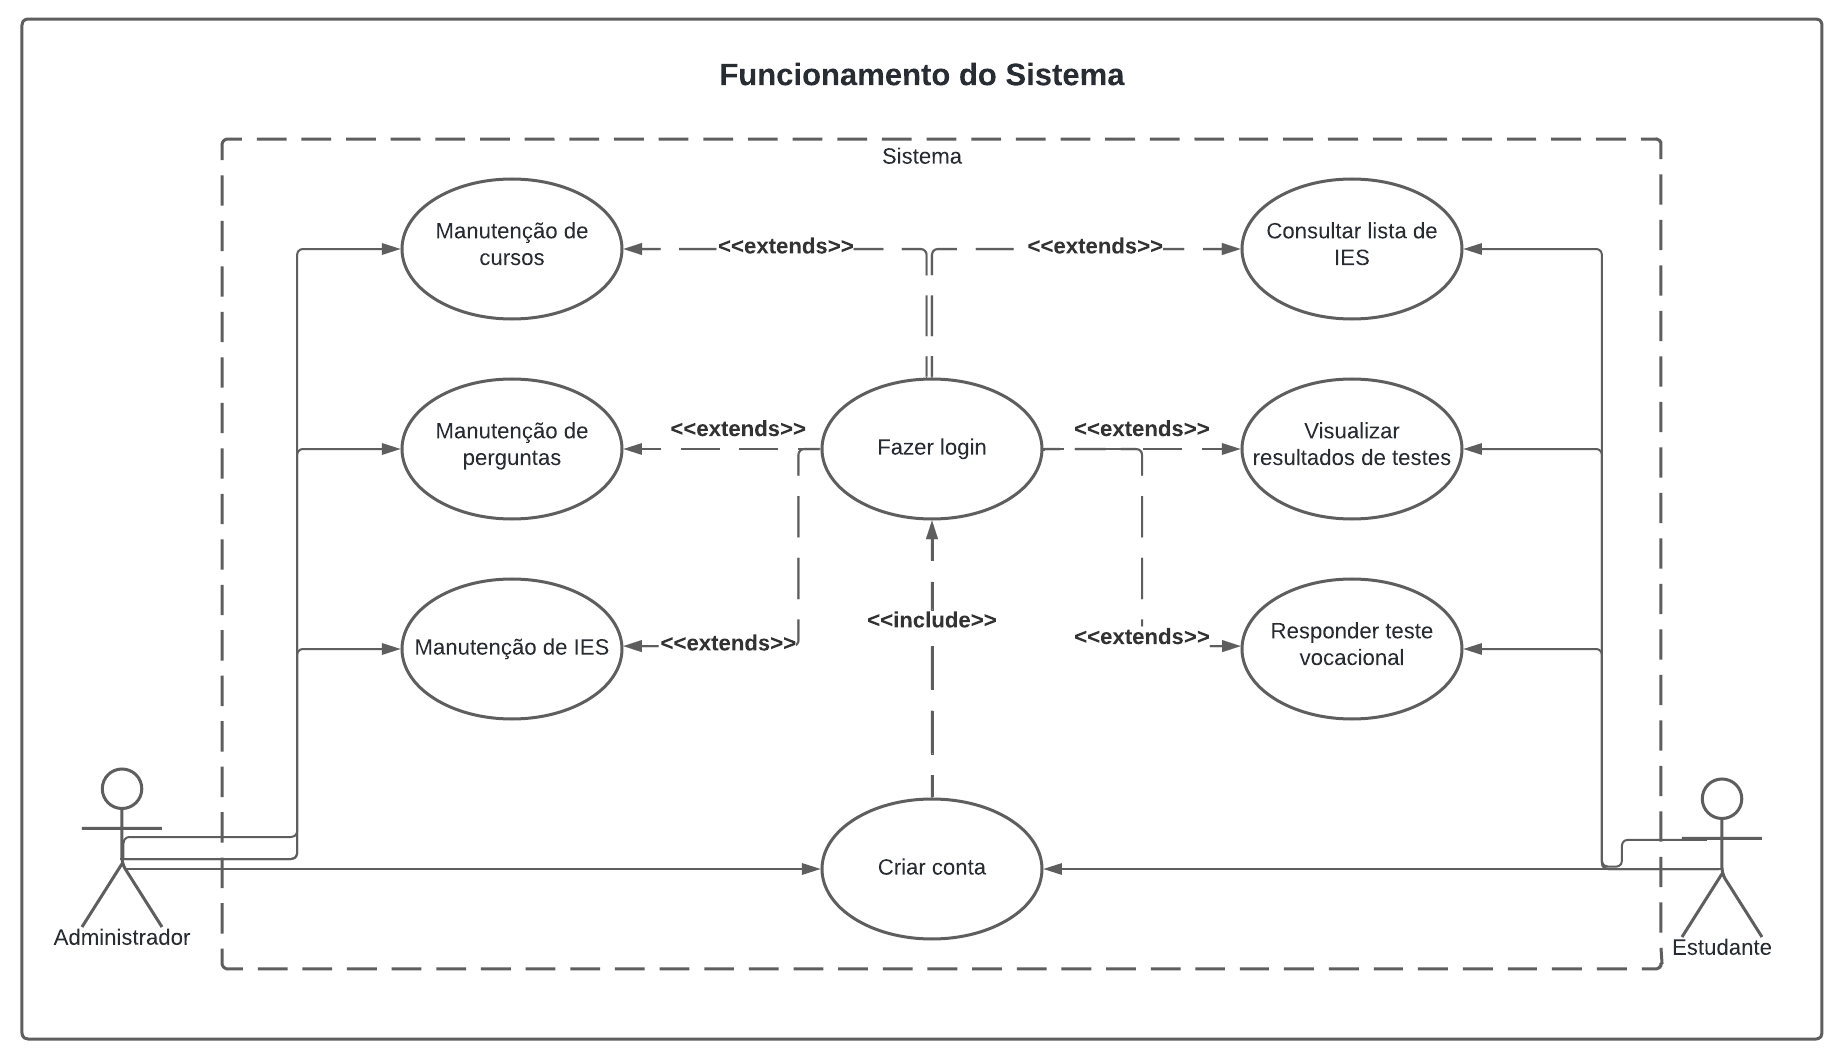
\includegraphics[scale=0.6]{images/caso-de-uso-funcionamento-sistema.png}
    \caption{Caso de Uso: Funcionamento do Sistema}
    \label{casodeuso}
\end{figure}  


\begin{table}[h!]
\centering
\caption{Fluxo de Cadastro de Usuário (Administrador)}
\begin{tabular}{|m{4cm}|m{11cm}|}
\hline
\textbf{Caso de Uso}   & \textbf{Cadastro de Usuário - Administrador} \\
\hline
Ator Principal & Administrador\\
\hline
Interessados e Interesses & O administrador deseja criar e gerenciar sua conta para acessar as funcionalidades de manutenção das perguntas do teste vocacional. \\
\hline
Pré-Condições & O administrador possui permissão para ter um cadastro na plataforma. \\
\hline
Fluxo Básico & 

1. O administrador acessa a página de cadastro.
2. O sistema solicita dados pessoais.
3. O administrador insere os dados.
4. O sistema valida os dados.
5. O sistema verifica se o e-mail é único.
6. O sistema salva os dados.
7. O administrador recebe confirmação de sucesso.\\
\hline
Fluxos Alternativos & 

1. E-mail já em uso: mensagem de erro.
2. E-mail inválido: mensagem de erro.
3. CPF inválido: mensagem de erro.
4. Campos obrigatórios não preenchidos: mensagem de erro.
\\
\hline
Fluxo de Exceção & Falha técnica: mensagem de erro, caso de uso encerrado. \\
\hline
Pós-Condições & Cadastro realizado com sucesso e administrador pode acessar a plataforma. \\
\hline
\end{tabular}
\label{table:casos-de-uso}
\\[1ex]
\footnotesize \textbf{Fonte}: Elaborado pelo autor.
\end{table}



\begin{table}[h!]
\centering
\caption{Fluxo de Cadastro de Instituição Pública}
\begin{tabular}{|m{4cm}|m{11cm}|}
\hline
\textbf{Caso de Uso}   & \textbf{Cadastro de Instituição Pública} \\
\hline
Ator Principal & Administrador\\
\hline
Interessados e Interesses & O administrador deseja cadastrar uma instituição pública na plataforma para disponibilizar informações sobre seus cursos, formas de ingresso e políticas públicas de acesso e permanência. \\
\hline
Pré-Condições & 

1. O administrador possui cadastro na plataforma.
2. A instituição possui as informações necessárias para cadastro.
\\
\hline
Fluxo Básico & 

1. O administrador acessa a funcionalidade de cadastro de instituição.
2. O sistema solicita os dados da instituição.
3. O administrador preenche os dados.
4. O sistema valida os dados.
5. O sistema valida e verifica a unicidade dos dados.
6. O sistema salva os dados.
7. O administrador recebe confirmação de sucesso.
\\
\hline
Fluxos Alternativos & 

1. Nome da instituição já em uso: mensagem de erro.
2. Site inválido: mensagem de erro.
3. Nota do MEC inválida: mensagem de erro.
4. Endereço incompleto: mensagem de erro.
\\
\hline
Fluxo de Exceção & Falha técnica: mensagem de erro, caso de uso encerrado. \\
\hline
Pós-Condições & Instituição pública cadastrada com sucesso na plataforma. \\
\hline
\end{tabular}
\label{table:casos-de-uso}
\\[1ex]
\footnotesize \textbf{Fonte}: Elaborado pelo autor.
\end{table}

\begin{table}[h!]
\centering
\caption{Fluxo de Cadastro de Usuário (Estudante)}
\begin{tabular}{|m{4cm}|m{11cm}|}
\hline
\textbf{Caso de Uso}   & \textbf{Cadastro de Usuário - Estudante} \\
\hline
Ator Principal & Estudante\\
\hline
Interessados e Interesses & O estudante deseja se cadastrar na plataforma para ter acesso ao teste vocacional personalizado e às informações sobre as universidades públicas. \\
\hline
Pré-Condições & O estudante possui mais de 14 anos de idade. \\
\hline
Fluxo Básico & 

1. O estudante acessa a página de cadastro.
2. O sistema solicita dados pessoais.
3. O estudante insere os dados.
4. O sistema valida os dados.
5. O sistema cria a conta e salva os dados.
6. O estudante recebe confirmação de sucesso.
\\
\hline
Fluxos Alternativos & 

1. E-mail inválido: mensagem de erro.
2. Campos obrigatórios não preenchidos: mensagem de erro.
4. Campos obrigatórios não preenchidos: mensagem de erro.
\\
\hline
Fluxo de Exceção & Falha técnica: mensagem de erro, caso de uso encerrado. \\
\hline
Pós-Condições & Cadastro realizado com sucesso e estudante pode acessar a plataforma. \\
\hline
\end{tabular}
\label{table:casos-de-uso}
\\[1ex]
\footnotesize \textbf{Fonte}: Elaborado pelo autor.
\end{table}

\newpage
\begin{table}[h!]
\centering
\caption{Fluxo de Manter Perguntas do Teste Vocacional}
\begin{tabular}{|m{4cm}|m{11cm}|}
\hline
\textbf{Caso de Uso}   & \textbf{Manter Perguntas do Teste Vocacional} \\
\hline
Ator Principal & Administrador\\
\hline
Interessados e Interesses & O administrador deseja gerenciar as perguntas do teste vocacional para garantir a qualidade e relevância do teste para os estudantes. \\
\hline
Pré-Condições & 

1. O administrador possui acesso ao sistema.
2. Deve haver ao menos uma pergunta cadastrada para alterar/excluir. \\
\hline
Fluxo Básico & 

1. O administrador acessa a funcionalidade de manutenção de perguntas.
2. O sistema exibe a lista de perguntas.
3. O administrador escolhe incluir, alterar, excluir ou consultar uma pergunta.
4. O sistema executa a ação e atualiza a lista.
\\
\hline
Fluxos Alternativos & 

1. Pergunta com texto vazio: mensagem de erro.
2. Pergunta inexistente: mensagem de erro na alteração/exclusão.
\\
\hline
Fluxo de Exceção & Falha técnica: mensagem de erro, caso de uso encerrado. \\
\hline
Pós-Condições & Pergunta incluída, alterada, excluída ou consultada com sucesso, mantendo a qualidade do teste.\\
\hline
\end{tabular}
\label{table:casos-de-uso}
\\[1ex]
\footnotesize \textbf{Fonte}: Elaborado pelo autor.
\end{table}

\begin{table}[h!]
\centering
\caption{Fluxo de Manter Informações sobre Cursos}
\begin{tabular}{|m{4cm}|m{11cm}|}
\hline
\textbf{Caso de Uso}   & \textbf{Manter Informações sobre Cursos} \\
\hline
Ator Principal & Administrador\\
\hline
Interessados e Interesses & O administrador deseja manter informações atualizadas sobre os cursos oferecidos pela instituição pública na plataforma. \\
\hline
Pré-Condições & 

1. O administrador possui acesso à plataforma.
2. A instituição já está cadastrada. \\
\hline
Fluxo Básico & 
1. O administrador acessa a funcionalidade de manutenção de cursos.
2. O sistema apresenta a lista de cursos.
3. O administrador escolhe incluir, alterar, excluir ou consultar um curso.
4. O sistema executa a ação e atualiza a lista.
\\
\hline
Fluxos Alternativos & 

1. Informações incompletas/ inválidas: mensagem de erro na inclusão.
2. Curso inexistente: mensagem de erro na alteração/exclusão.
\\
\hline
Fluxo de Exceção & Falha técnica: mensagem de erro, caso de uso encerrado. \\
\hline
Pós-Condições & Informações sobre os cursos atualizadas com sucesso, permitindo consulta pelos usuários.\\
\hline
\end{tabular}
\label{table:casos-de-uso}
\\[1ex]
\footnotesize \textbf{Fonte}: Elaborado pelo autor.
\end{table}

\begin{table}[h!]
\centering
\caption{Fluxo de Responder o Teste Vocacional}
\begin{tabular}{|m{4cm}|m{11cm}|}
\hline
\textbf{Caso de Uso}   & \textbf{Responder o Teste Vocacional} \\
\hline
Ator Principal & Estudante\\
\hline
Interessados e Interesses & O estudante deseja responder ao teste vocacional disponibilizado pela plataforma. \\
\hline
Pré-Condições & 

O estudante deve estar autenticado no sistema. \\
\hline
Fluxo Básico & 
1. O estudante acessa a funcionalidade de responder ao teste.
2. O sistema apresenta as perguntas.
3. O estudante responde às perguntas.
4. O estudante finaliza o teste.
5. O sistema registra as respostas no banco de dados.
\\
\hline
Fluxos Alternativos & 

1. Teste interrompido: sistema preserva respostas parciais, mas só armazena após a conclusão do teste.
\\
\hline
Fluxo de Exceção & Falha técnica: mensagem de erro, estudante pode tentar novamente após resolução do problema. \\
\hline
Pós-Condições & Respostas registradas no sistema para gerar recomendações de cursos.\\
\hline
\end{tabular}
\label{table:casos-de-uso}
\\[1ex]
\footnotesize \textbf{Fonte}: Elaborado pelo autor.
\end{table}

\begin{table}[h!]
\centering
\caption{Fluxo de Apresentar Recomendação de Curso}
\begin{tabular}{|m{4cm}|m{11cm}|}
\hline
\textbf{Caso de Uso}   & \textbf{Apresentar Recomendação de Curso} \\
\hline
Ator Principal & Sistema\\
\hline
Interessados e Interesses & O sistema precisa fornecer uma recomendação personalizada de cursos para o estudante com base nas respostas do teste vocacional, auxiliando-o na escolha de sua formação acadêmica. \\
\hline
Pré-Condições & 

1. O estudante realizou o teste vocacional.
2. O sistema possui algoritmos de análise e recomendação configurados. \\
\hline
Fluxo Básico & 
1. O sistema analisa as respostas do teste vocacional.
2. O sistema gera uma recomendação personalizada de cursos.
3. O sistema apresenta a recomendação ao estudante.
4. O sistema armazena a recomendação no banco de dados.
\\
\hline
Fluxos Alternativos & 

1. Algoritmo de recomendação falha: sistema exibe uma mensagem de erro e sugere tentar novamente mais tarde.
\\
\hline
Fluxo de Exceção & Falha técnica: mensagem de erro, estudante pode tentar novamente após resolução do problema. \\
\hline
Pós-Condições & Recomendação de curso gerada e apresentada ao estudante.\\
\hline
\end{tabular}
\label{table:casos-de-uso}
\\[1ex]
\footnotesize \textbf{Fonte}: Elaborado pelo autor.
\end{table}

\clearpage

\section{Volumetria}

Para a fase inicial do projeto, estimamos a seguinte volumetria de dados para a plataforma:

\begin{itemize}
\item Estudantes: A aplicação será lançada sem estudantes cadastrados.
\item Administradores: Começaremos com 5 administradores cadastrados, que são os membros integrantes do projeto.
\item Instituições: Inicialmente, todas as universidades federais do Brasil serão cadastradas, totalizando 69 instituições.
\item Áreas: A aplicação iniciará com 12 áreas cadastradas. 
\item Cursos: A aplicação iniciará com 50 cursos cadastrados. 
\item Políticas Públicas: A aplicação será lançada com 20 políticas públicas cadastradas, relacionadas com as instituições que as possuem.
\item Testes Vocacionais: Disponibilizaremos inicialmente uma única opção de teste vocacional para os usuários.
\item Perguntas: O teste vocacional inicialmente terá 30 perguntas.
\item Perfis: Para recomendar cursos aos usuários, utilizaremos os 6 perfis definidos pela Teoria de Escolhas Vocacionais de John Holland.
\end{itemize}

De acordo com o número de registros estimados, o espaço ocupado no nosso banco de dados no momento de lançamento da plataforma será aproximadamente 3 MB.  Optamos por iniciar com esse volume de dados por ser adequado para a fase inicial do projeto. No entanto, é importante destacar que haverá uma expansão desses dados em futuras entregas da aplicação, conforme será detalhado no Capítulo \ref{escolhas-descartes}, Seção 5.3.


\section{Arquitetura}

Nesse projeto, a \textbf{Clean Architecture} foi escolhida como a base para o desenvolvimento do \textit{software}, refletindo a necessidade de criar um sistema que seja ao mesmo tempo flexível e de fácil manutenção. A adoção desta abordagem foi motivada pela sua capacidade de promover uma separação clara e eficiente entre diferentes camadas do sistema, como entidades de negócio, casos de uso, interfaces de usuário e infraestrutura. Essa estrutura não só garante uma organização modular do código, mas também facilita a realização de testes automatizados em cada camada, assegurando a qualidade e permitindo a detecção precoce de problemas.

A Clean Architecture permite que as regras de negócio sejam desacopladas das tecnologias específicas, o que confere ao sistema uma maior adaptabilidade às mudanças futuras. Isso é crucial para a evolução contínua e sustentável do software. No entanto, a implementação dessa arquitetura não foi isenta de desafios. A necessidade de definir claramente as responsabilidades de cada camada de forma a seguir o princípio de responsabilidade única e garantir uma comunicação eficaz entre elas exigiu planejamento e atenção aos detalhes. Além disso, a adoção de uma arquitetura modular impôs um esforço adicional na integração de componentes e na garantia de que as interfaces entre as camadas fossem bem projetadas e funcionais. Esses desafios foram superados por meio de uma abordagem iterativa e de refinamento contínuo, que assegurou que a arquitetura atendesse às necessidades do projeto e suportasse a evolução do software de maneira eficiente.


Na Figura \ref{arquitetura} é possível observar a representação em diagrama da arquitetura escolhida para a aplicação. 

\begin{figure}[ht]
        \centering
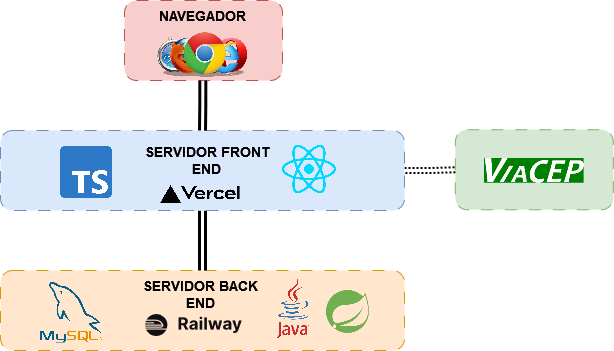
\includegraphics[width=0.8\textwidth]{images/EstruturaVocco(1).png}
        \caption{Arquitetura da aplicação}
        \label{arquitetura}
    \end{figure}

A seguir detalharemos cada uma das tecnologias escolhidas e como será feita a comunicação entre elas.

\subsection{Back-End}
No que diz respeito ao \textit{back-end}, adotamos o \textit{framework} \textbf{Spring Boot} em conjunto com a arquitetura \ac{msc}. O Spring Boot é uma escolha popular para o desenvolvimento de aplicativos Java devido à sua facilidade de configuração e rápida inicialização, como discutido nas Subseçõs 5.1.1 e 5.1.2 do Capítulo \ref{escolhas-descartes}. A arquitetura \ac{msc} divide a aplicação em três camadas distintas: \textbf{Model}, onde definimos as entidades e regras de negócio; \textbf{Service}, responsável pela lógica de negócio e manipulação dos dados; e \textbf{Controller}, que recebe as requisições \ac{http} e coordena a interação entre o cliente e o servidor. 

Além das camadas Model, Service e Controller, também implementamos a camada \textbf{Repository} como parte da arquitetura \ac{msc}. A camada Repository é responsável pela interação com o banco de dados, encapsulando a lógica de acesso e manipulação dos dados. Utilizando interfaces e métodos específicos, o Repository abstrai as operações \ac{crud}, permitindo que as demais camadas da aplicação interajam com o banco de dados de forma desacoplada e eficiente.

A utilização da arquitetura em camadas proporcionou diversos benefícios para o projeto. Em primeiro lugar, a separação de responsabilidades entre as camadas Model, Service, Controller e Repository facilitou a organização e compreensão do código-fonte, tornando-o mais legível e manutenível. Cada camada possui um propósito claro e bem definido, o que simplifica o processo de desenvolvimento e permite que diferentes equipes ou desenvolvedores trabalhem de forma independente em áreas específicas da aplicação.

\subsubsection{Gerenciamento de dependências}
Para o gerenciamento de dependências do projeto, optamos pelo \textbf{Maven}. Esta escolha se baseia nos inúmeros benefícios oferecidos por essa ferramenta. O Maven simplifica a gestão de dependências, permitindo que as bibliotecas necessárias sejam facilmente adicionadas ao projeto através de seu arquivo de configuração padrão (pom.xml). Além disso, o Maven automatiza tarefas como compilação, empacotamento e distribuição do projeto, tornando o processo de desenvolvimento mais eficiente e menos propenso a erros. Sua vasta gama de plugins oferece funcionalidades adicionais, como integração com ferramentas de teste e análise de código, promovendo uma abordagem mais completa para o desenvolvimento de \textit{software}. 

\subsection{Front-End}
Nesse projeto, optamos por utilizar \textbf{React} em conjunto com \textbf{TypeScript} para o desenvolvimento do \textit{front-end}. Essa escolha foi motivada pela necessidade de construir uma interface de usuário dinâmica e reativa, com uma base de código robusta e escalável, conforme discutido nas Subseções 5.1.3 e 5.1.4 do Capítulo \ref{escolhas-descartes}, onde são abordadas a adoção do TypeScript e a utilização do React para garantir produtividade, qualidade do código. O React é uma biblioteca JavaScript amplamente adotada que nos permite criar componentes reutilizáveis e composicionais, facilitando a construção de interfaces complexas de forma modular. Além disso, a integração com TypeScript adiciona um sistema de tipos estáticos ao JavaScript, oferecendo benefícios como detecção de erros em tempo de compilação e melhorando a manutenibilidade do código. A arquitetura baseada em componentes nos permitiu organizar a aplicação de forma hierárquica, facilitando a manutenção e o teste dos diferentes elementos da interface.

Na figura \ref{aplicação}, é possível ver o QRcode da aplicação que foi publicada na internet:

\begin{figure}[ht]
        \centering
        \href{https://vocco.vercel.app}{
\includegraphics[width=0.5\textwidth]{images/qrcode-url-aplicacao.png}}
        \caption{QRcode URL da Aplicação}
        \label{aplicação}
\end{figure}
\href{https://vocco.vercel.app}{https://vocco.vercel.app}

\newpage
\subsection{Banco de dados}
Em relação ao banco de dados,  optamos pelo \textbf{MySQL} devido à sua confiabilidade, desempenho e ampla adoção na indústria. O MySQL é um sistema de gerenciamento de banco de dados relacional que oferece recursos avançados de segurança e escalabilidade, sendo uma escolha sólida para aplicações de diferentes tamanhos e complexidades. Utilizamos o MySQL para armazenar e gerenciar os dados da aplicação, garantindo a integridade e disponibilidade das informações.


\subsubsection{Modelo Entidade Relacionamento}

O \ac{mer} é uma ferramenta fundamental no design de bancos de dados, pois permite visualizar de forma clara as relações entre as diversas entidades do domínio do sistema. O \ac{mer} da plataforma Vocco pode ser observado na Figura \ref{mer}.

\newpage
\begin{figure}[ht]
        \centering
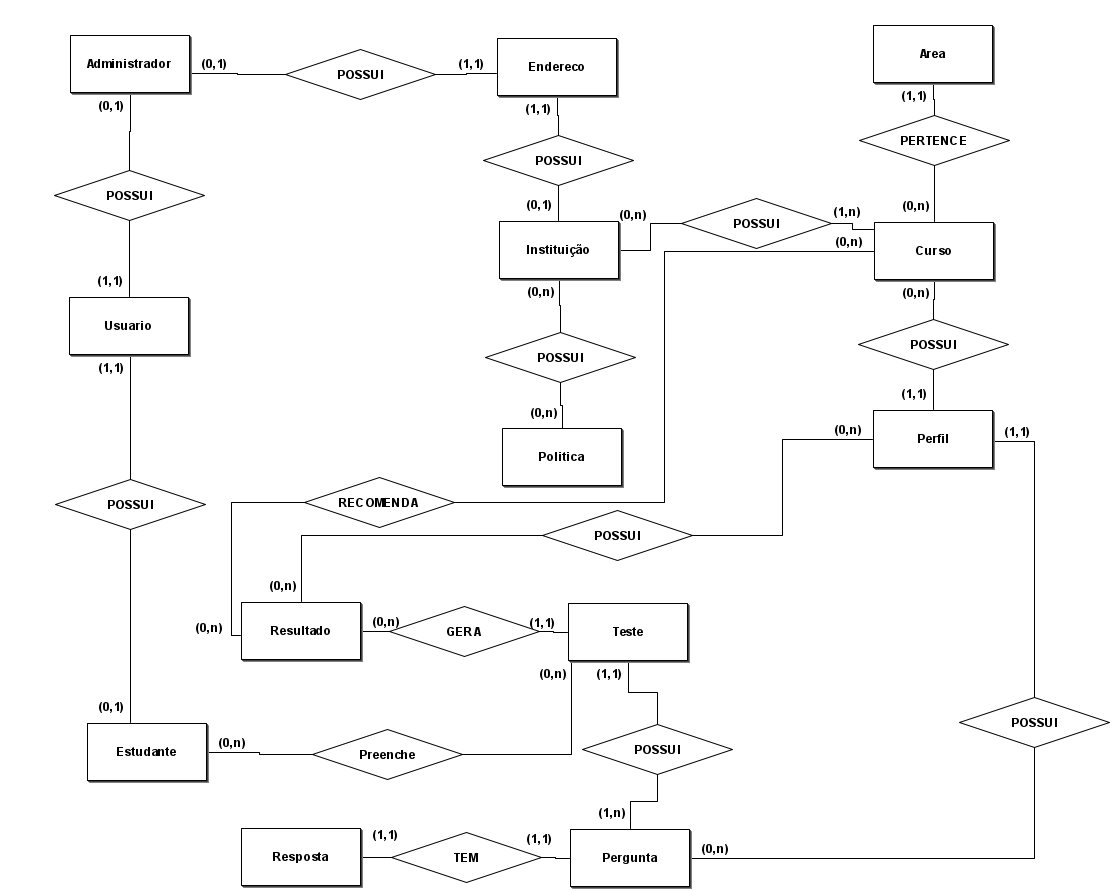
\includegraphics[width=1.0\textwidth]{images/mer.png}
        \caption{Modelo Entidade Relacionamento (MER) do projeto}
        \label{mer}
    \end{figure}
    
No processo de elaboração do diagrama, nosso foco primordial reside na visualização das relações entre as tabelas. Esse enfoque nos capacitou a estabelecer um sistema com informações confiáveis e interligadas, fundamentais para garantir a integridade e a eficácia dos dados. 

\newpage

\subsubsection{Diagrama Entidade Relacionamento}

O \ac{der} é uma ferramenta muito importante na modelagem de dados. Ele oferece uma visão clara das entidades, seus atributos e como elas se relacionam. Uma técnica central no \ac{der} é o uso de chaves estrangeiras para mapear as relações entre tabelas. Essas chaves garantem a integridade referencial entre os dados, assegurando que cada registro em uma tabela relacionada possa ser corretamente associado a outro em uma tabela diferente. O \ac{der} da plataforma Vocco pode ser observado na Figura \ref{der}

\begin{figure}[ht]
        \centering
        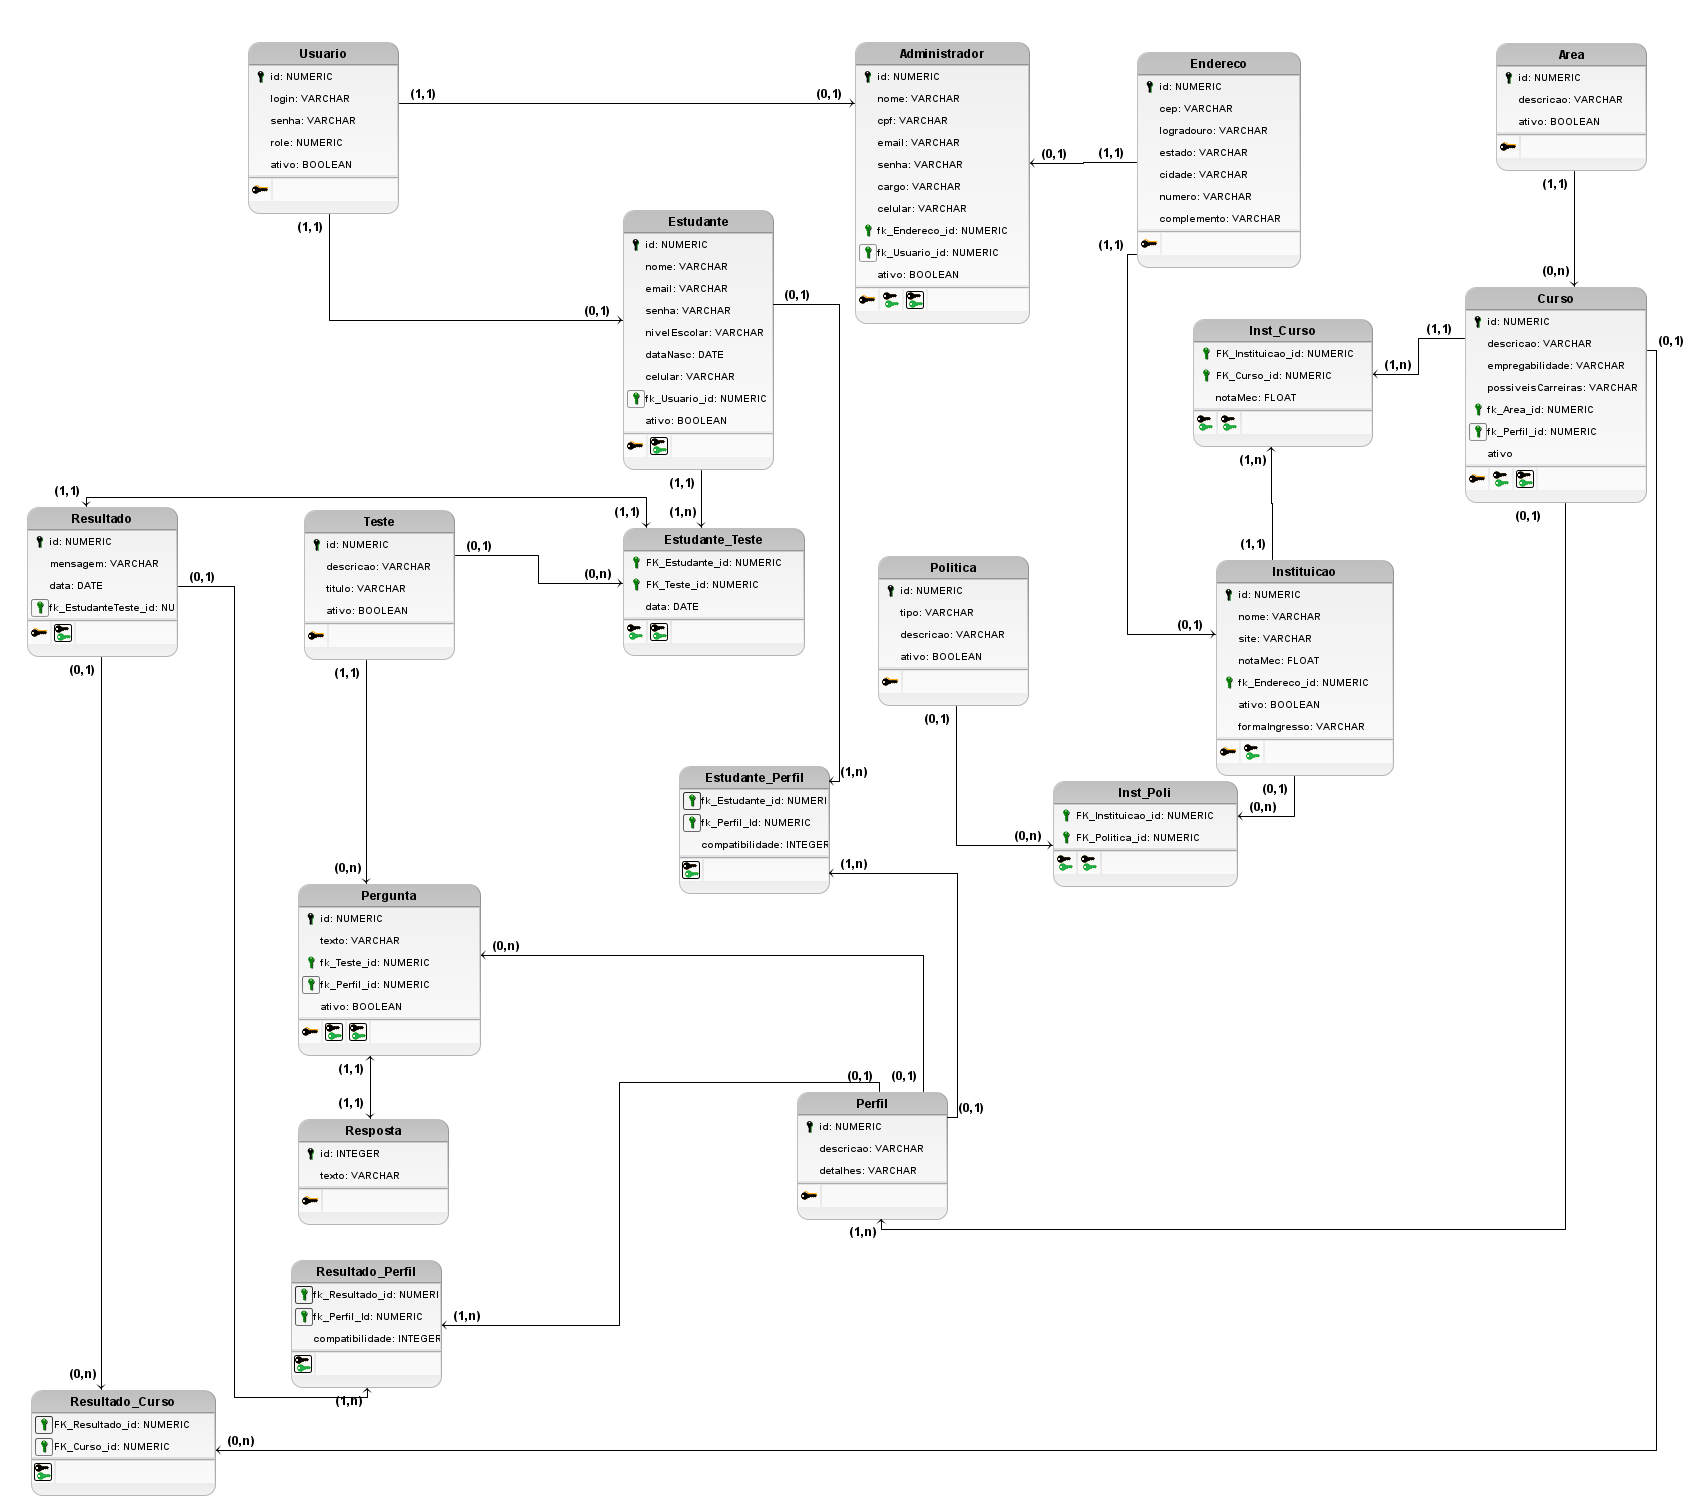
\includegraphics[width=1.0\textwidth]{images/der.png}
        \caption{Diagrama Entidade Relacionamento (DER) do projeto}
        \label{der}
    \end{figure}
    
Este diagrama oferece uma visão clara do processo de mapeamento dos relacionamentos entre as tabelas do banco de dados. Seguimos um padrão que envolve a criação de entidades associativas para representar os relacionamentos N-N. Para os relacionamentos 1-N, adicionamos a chave estrangeira na tabela que recebe o 'N' no mapeamento. Quanto aos relacionamentos 1-1 e 0-1, a escolha da tabela que recebe a chave estrangeira foi feita com base no que a equipe considerou mais relevante, levando em conta os requisitos específicos da plataforma.

\subsection{Integrações}
Para aprimorar a experiência do usuário e garantir a precisão dos dados de endereço nos cadastros, optamos por integrar a \ac{api} do \textbf{ViaCEP}. Essa integração permite que, ao preencher os campos de endereço em formulários de cadastro, o sistema automaticamente consulte a \ac{api} do ViaCEP para obter informações detalhadas, como rua, bairro, cidade e estado, com base no \ac{cep} fornecido pelo usuário. Essa abordagem simplifica e agiliza o processo de preenchimento dos cadastros, além de garantir a consistência e atualização dos dados de endereço. Ao utilizar essa \ac{api}, estamos priorizando a precisão e a eficiência na coleta e manipulação das informações de endereço, proporcionando uma experiência mais fluida e intuitiva para os usuários.

\subsection{Infraestrutura}
Por fim, para hospedar nosso projeto, optamos por utilizar serviços de hospedagem em nuvem para abrigar tanto o \textit{front-end} quanto o \textit{back-end}. Essa escolha foi motivada por diversos fatores que visam garantir uma maior eficiência e escalabilidade do sistema.

Primeiramente, a hospedagem em nuvem oferece uma infraestrutura altamente flexível, permitindo ajustes rápidos de recursos conforme a demanda do aplicativo. Além disso, ela proporciona uma maior disponibilidade e confiabilidade, com garantias de tempo de atividade elevado e redundância de dados. A facilidade de implementação e gerenciamento também foi considerada, já que a infraestrutura em nuvem permite uma rápida implantação e manutenção simplificada do sistema.

Por fim, os custos operacionais são otimizados, pois os serviços em nuvem geralmente seguem um modelo de pagamento conforme o uso, evitando gastos excessivos com infraestrutura desnecessária.

\subsection{Front - End}
Para hospedar o \textit{front-end}, escolhemos a plataforma \textbf{Vercel}, conhecida por sua facilidade de uso e escalabilidade. O \textit{front-end} foi desenvolvido com React e TypeScript, aproveitando os benefícios de uma tipagem estática para garantir um código mais robusto e menos propenso a erros. O uso do Vite como \textit{bundler} permitiu um processo de desenvolvimento mais rápido e eficiente, gerando builds otimizados e facilitando a implementação de novas funcionalidades. 

Além disso, é importante destacar que o \textit{front-end} se conecta ao \textit{back-end} através de requisições \ac{https}, garantindo a segurança e integridade dos dados transmitidos entre as partes. Essa abordagem assegura uma comunicação confiável e protegida entre os diferentes componentes do sistema, contribuindo para uma experiência segura e estável para os usuários.

\subsubsection{Back - End}
Para hospedar o \textit{back-end}, foi escolhida a plataforma \textbf{Railway}, conhecida por sua eficiência e facilidade de integração. Para o gerenciamento do banco de dados, optamos pelo MySQL, um sistema robusto e amplamente utilizado. A integração entre o Spring Boot e o MySQL foi facilitada através de um container Docker, gerado automaticamente pela plataforma Railway, proporcionando uma configuração que garante a conexão eficiente entre o \textit{core} da nossa aplicação e os dados persistidos, sendo que a conexão entre a aplicação e o banco foi realizada utilizando variáveis de ambiente definidas dentro do Railway, aumentando a segurança e confiabilidade. 



\subsection{Escalabilidade}
A escalabilidade é crucial para garantir que a Vocco possa se adaptar ao crescimento de forma eficaz, mantendo flexibilidade, confiabilidade, eficiência e manutenibilidade. Acreditamos  que tais metas serão alcançadas por meio de nossas decisões de utilizar serviços em nuvem e um sistema gerenciador de banco de dados que facilite o processo de expansão do nosso sistema. Neste momento, nosso foco está em manter uma \textbf{escalabilidade vertical}, o que implica em aumentar a capacidade de armazenamento em vez de adicionar mais servidores. Essa abordagem nos permite otimizar recursos e simplificar o gerenciamento, garantindo que Vocco possa se adaptar ao crescimento de maneira ágil e econômica.
\subsection{Controle de versão}
 No desenvolvimento deste projeto, optamos por utilizar tanto o \textbf{Git} como o \textbf{GitHub} para o controle de versão do código-fonte. O Git foi escolhido como sistema de controle de versão devido à sua eficiência e robustez no gerenciamento de alterações de código, permitindo o acompanhamento do histórico de modificações, a colaboração entre os membros da equipe e a criação de branches para o desenvolvimento de novas funcionalidades de forma isolada. Além disso, o GitHub foi utilizado como plataforma de hospedagem remota dos repositórios Git, proporcionando uma maneira conveniente de compartilhar o código entre os membros da equipe, revisar alterações, gerenciar problemas e automatizar processos de \ac{ci} e \ac{cd}.

 Na figura \ref{github}, é possível acessar o nosso repositório do GitHub do projeto: 

\begin{figure}[ht]
        \centering
        \href{https://github.com/betatrix/Projeto-Integrado-I}{
        
\includegraphics[width=0.5\textwidth]{images/qrcode-repo-github.png}
        }
        \caption{QRcode Repositório do GitHub}
        \label{github}
\end{figure}
 
 A utilização do Git e do GitHub garante que os membros da equipe colaborem de maneira eficaz e organizada, mantendo o código atualizado e permitindo uma gestão eficiente das tarefas e do progresso do projeto.

\section{Manutenibilidade}

A manutenibilidade de um \textit{software} refere-se à facilidade com que ele pode ser mantido e modificado ao longo do tempo. Em outras palavras, é a capacidade do sistema de ser compreendido, adaptado, corrigido e aprimorado de maneira eficiente e econômica. A manutenibilidade é uma característica fundamental de qualidade do \textit{software}, pois afeta diretamente a capacidade da equipe de desenvolvimento de responder a novos requisitos, corrigir falhas e melhorar a funcionalidade do sistema ao longo do ciclo de vida do \textit{software}.

\subsection{Code Convention}
A adoção de convenções de código padronizadas é fundamental para garantir a legibilidade, consistência e manutenção eficiente do software. Este capítulo aborda as práticas recomendadas e as diretrizes específicas que devem ser seguidas por todos os desenvolvedores do projeto ao escrever e revisar o código.

\begin{itemize}
    \item \textbf{Back-End}
     Seguiremos as convenções de código  para a linguagem Java conforme estabelecidas na documentação oficial da Oracle. Algumas das principais orientações incluem:
     \begin{itemize}
        \item \textbf{Nomenclatura de Classes, Interfaces e Tipos:}
        Utilizar PascalCase, começando com letra maiúscula;
        \item \textbf{Nomenclatura de Métodos e Variáveis:}
        Utilizar camelCase, começando com letra minúscula;
        \item \textbf{Constantes e variáveis:}
        Utilizar letras maiúsculas separadas por sublinhados;
        \item \textbf{Indentação:}
        Utilizar quatro espaços para indentação e evitar o uso de tabulação;
        \item \textbf{Comentários:}
        Explicar trechos de código complexos ou documentar \ac{api};
        \item \textbf{Linhas de Comprimento:}
         Limitar o comprimento a 80-100 caracteres para melhorar a legibilidade;
        \item \textbf{Imports:}
        Evitar importar pacotes inteiros, trazendo apenas classes específicas ou utilizar asterisco apenas para \textit{imports} estáticos.
     \end{itemize}
\end{itemize}
\begin{itemize}
    \item \textbf{Front-End}
     Para o desenvolvimento \textit{front-end}, adotaremos as principais convenções de código:
     \begin{itemize}
        \item \textbf{Nomenclatura de variáveis:}
        Utilizaremos camelCase, começando com letra minúscula;
        \item \textbf{Nomenclatura de funções:}
        Utilizaremos PascalCase, começando com letra maiúscula;
        \item \textbf{Declaração de variáveis:}
        Preferimos utilizar \textbf{let} ou \textbf{const} em vez de \textbf{var} para declarar variáveis, pois isso ajuda a evitar problemas de escopo;
        \item \textbf{Convenções de nome para constantes:}
        Nomearemos constantes utilizando letras maiúsculas e palavras separadas por sublinhados;
        \item \textbf{Comentários:}
        Faremos uso de comentários para documentar o código, explicando o propósito de funções e partes importantes do código;
        \item \textbf{Tratamento de erros:}
        Faremos uso de blocos try-catch para capturar e lidar com exceções, quando necessário;
        \item \textbf{Ponto e vírgula:}
         Apesar de o JavaScript permitir a omissão de ponto e vírgula no final das declarações, incluiremos sempre para evitar comportamentos inesperados;
        \item \textbf{Uso de aspas:}
        Utilizaremos aspas duplas de forma consistente para \textit{strings}.
 
     \end{itemize}
\end{itemize}
\subsection{Ferramentas de testes}

Os testes de \textit{software} são uma etapa fundamental no ciclo de desenvolvimento de \textit{software}, cujo objetivo é garantir a qualidade e a confiabilidade do produto final. Essas atividades consistem em verificar se o \textit{software} atende aos requisitos estabelecidos, se funciona corretamente em diferentes cenários de uso e se está livre de defeitos e erros. Os testes de \textit{software} podem abranger diversas áreas, como funcionalidade, desempenho, segurança e usabilidade, e são conduzidos por meio de técnicas e ferramentas específicas. 

Para a realização dos testes utilizaremos as seguintes ferramentas:
 
\begin{itemize}
    \item \textbf{JUnit:}
     Será utilizado no \textit{back-end} o \textit{framework} JUnit como ferramenta de testes automatizados. Ele oferece recursos que facilitam a criação e execução de testes, incluindo suporte para testes parametrizados, testes de exceção e integração com ferramentas que utilizaremos para o desenvolvimento.
    \item \textbf{Jest:}
    Para os testes automatizados no \textit{front-end}, escolhemos o Jest como nossa ferramenta principal. Ele abrange uma ampla gama de cenários de teste, desde os unitários mais simples até os de integração mais complexos, destacando-se pela sua facilidade e rapidez de uso. 
    \item \textbf{Typescript EsLint:}
    Para conduzir uma análise estática abrangente em nosso \textit{front-end}, decidimos adotar o TypeScript ESLint. Essa escolha se deve ao fato de que essa ferramenta combina as vantagens de \textit{linting} de código, e nos permite definir regras personalizadas, garantindo que sigamos as melhores práticas e padrões de codificação estabelecidos.
    \item \textbf{SonarQube:}
    Utilizaremos o SonarQube como nossa ferramenta de análise estática do \textit{back-end}. Ele realiza uma avaliação detalhada do código, identificando potenciais problemas, vulnerabilidades de segurança, \textit{bugs}, duplicações de código e padrões de código não conformes.
\end{itemize}
\subsection{Design Patterns}
Optamos por adotar o padrão \textbf{SOLID} como base para o desenvolvimento deste sistema, pois ele encapsula um conjunto de cinco princípios essenciais de design de software, idealizados por Robert C. Martin. Esses princípios são fundamentais para criar um código mais limpo, modular e fácil de manter. Ao seguirmos esses princípios, garantimos que nossas classes e módulos tenham responsabilidades bem definidas, promovendo a coesão e o baixo acoplamento, o que facilita tanto a compreensão do código quanto sua manutenção no futuro. 

Também utilizaremos o padrão \ac{dto} para permitir a comunicação eficiente de dados entre diferentes partes do nosso sistema. Para representar esses objetos de transferência de dados, optaremos por utilizar \textit{\textbf{records}}, aproveitando as suas vantagens de imutabilidade e clareza.

\section{Segurança, Privacidade e Legislação}
A segurança representa um aspecto essencial na arquitetura da Vocco. Dessa forma, nesta seção serão citadas as boas práticas e tecnologias usadas para garantir uma maior confiabilidade e segurança para os usuários de nossa aplicação.

\subsection{Lei Geral de Proteção de Dados (LGPD)}
A \ac{lgpd} (Congresso Nacional, 2018), foi promulgada com o objetivo de proteger os direitos fundamentais de liberdade e de privacidade, e a livre formação da personalidade de cada indivíduo, atuando sobre o tratamento de dados pessoais, incluindo em meios digitais.
Com isso, durante o planejamento da estruturação da plataforma, foram definidas ações visando atender a essas necessidades de segurança, para dessa forma assegurar que a aplicação estivesse em conformidade com essa legislação e atendendo ao compromisso de proteger nossos usuários.

A aplicação respeita o livre acesso a esses dados, definido no Art. 6\textsuperscript{o},IV, e requisitará consentimento dos usuários para armazenar os dados fornecidos, o que confere a ela conformidade com o Art. 7\textsuperscript{o}
,I.


\subsection{Autenticação e Autorização}
A aplicação conta com etapas de autenticação e autorização à depender do usuário e seus privilégios, para garantir maior privacidade à informações e também uma melhor gestão de como os recursos serão acessados tanto no \textit{back-end} como no \textit{front-end}.

A autenticação como sendo o login do usuário no sistema e a autorização como sendo o processo posterior, em que é verificado se o usuário tem permissão de acesso a um determinado recurso.
O Spring Security é um \textit{framework} do Java que possui um sistema  de autenticação e autorização para aplicações Java, como é o caso da Vocco, além disso conta com proteção contra ataques como \textit{session fixation}, \textit{clickjacking} e protege contra injeção de DDR, se mostrando uma ferramenta madura e qualificada para proteger a aplicação.

Para implementar o fluxo de autenticação, é usado o \textit{Bearer Token}, que é gerado após a validação das credenciais pelo \textit{back-end} Java Spring Boot, garantindo a autenticidade e evitando conflitos.
O \textit{Bearer Token} ou "token de portador", é um tipo de token de acesso usado para acessar recursos protegidos, como \ac{api}. Esse \textit{token} é gerado pelo servidor em resposta a uma solicitação de login, e deve ser incluído no cabeçalho de autorização das solicitações \ac{http} para recursos protegidos.


\subsection{Criptografia de Dados}
A criptografia é uma alternativa ideal para anonimização de dados, reduzindo as chances de violação de dados e as multas que a \ac{lgpd} pode impor. Desempenha um papel fundamental na proteção das informações, tornando-as ininteligíveis para terceiros não autorizados, impedindo que pessoas não autorizadas utilizem as informações para benefício próprio, embaralhando os dados de forma que não sejam legíveis, tanto por humanos quanto por sistemas projetados para interpretar informações.

Para aplicar essa medida de segurança na aplicação Vocco, será usada a ferramenta \textbf{BCrypt}, que tem o intuito de esconder senhas criadas pelos usuários em forma de texto “puro” em dados indecifráveis, utilizando o algoritmo \textit{hash}.
Será utilizada essa ferramenta para criptografar as senhas dos usuários no banco de dados. 


\section{Viabilidade Financeira}
A análise da viabilidade financeira demonstra o custo operacional estimado para o primeiro ano após o lançamento da plataforma. Esta avaliação considera os custos de mão de obra de desenvolvimento, registro de domínio, utilização dos serviços oferecidos pela plataforma de desenvolvimento na nuvem Railway para hospedar o \textit{back-end}, levando em conta um aumento de 30\% no processamento e uso dos recursos da mesma e também pela utilização da plataforma Vercel para hospedar o \textit{front-end}. Com base nesses parâmetros, segue a estimativa dos custos operacionais para o primeiro ano após o lançamento da plataforma.

\begin{table}[h!]
\centering
\caption{Estimativa dos Custos Operacionais}
\begin{tabular}{|m{5cm}|m{4cm}|m{4cm}|}
\hline
\textbf{Descrição}   & \textbf{Valor Anual (R\$)} & \textbf{Valor Mensal (R\$)} \\
\hline
Custo de Desenvolvimento & 42.240,00 & 3.520,00 \\
\hline
Registro de Domínio & 40,00 & 3,33 \\
\hline
Plataforma Railway & 702,92 & 58,58 \\
\hline
Plataforma Vercel & 1.225,2  & 102,10 \\
\hline
\textbf{Total} & \textbf{44.208,12} & \textbf{3.684,01} \\
\hline
\end{tabular}
\label{table:estimativa-custos}
\\[1ex]
\footnotesize \textbf{Fonte}: Elaborado pelo autor.
\end{table}

A estimativa dos custos operacionais detalhada, apresenta que o Custo de Desenvolvimento anual será calculado com base em 1.320 horas anuais de trabalho, cumpridas por uma gerente e quatro desenvolvedoras. A gerente será remunerada em R\$8,00 por hora, enquanto cada desenvolvedora será remunerada em R\$6,00 por hora. O valor de registro de domínio será de R\$40,00 o qual é uma taxa paga anualmente. Além disso, há o custo com a plataforma Railway em que são considerados os valores de utilização do plano mensal Hobby de R\$ 25,33, mais o valor adicional de R\$ 398,96 para o aumento de 30\% no uso dos recursos da plataforma, e esse valor é dividido em 12 meses. Por fim,  o custo com a plataforma Vercel será de R\$102,10 com o plano mensal Pró. Esses valores são apresentados  na Tabela \ref{table:detalhamento-custos} a seguir:

\begin{table}[h!]
\centering
\caption{Detalhamento dos Custos Operacionais}
\begin{tabular}{|m{4cm}|m{4cm}|m{3cm}|m{3cm}|}
\hline
\textbf{Item} & \textbf{Descrição} & \textbf{Valor Anual (R\$)} & \textbf{Valor Mensal (R\$)} \\
\hline
Desenvolvimento & 1 Gerente  & 10.560,00 & 880,00 \\
\hline
 Desenvolvimento & 4 Desenvolvedoras & 31.680,00 & 2.640,00 \\
\hline
Registro de Domínio & Plano Fixo Anual & 40,00 & 3,33 \\
\hline
Plataforma Railway & Plano mensal Hobby & 303,96 & 25,33 \\
\hline
Plataforma Railway & 30\% de uso adicional & 398,96 & 33,25 \\
\hline
Plataforma Vercel & Plano Pró & 1.225,20 & 102,10 \\
\hline
\textbf{Total} & & \textbf{44.208,12} & \textbf{3.684,01} \\
\hline
\end{tabular}
\label{table:detalhamento-custos}
\\[1ex]
\footnotesize \textbf{Fonte}: Elaborado pelo autor.
\end{table}

Dessa forma, a estimativa de Custo Operacional anual será de R\$44.208,12 e mensal de R\$3.684,01, como apresentado nas tabelas anteriores.


\subsection{Monetização}

A plataforma oferecerá suas funcionalidades gratuitamente, visando garantir a acessibilidade e engajamento dos usuários, porém apresentará campos com anúncios, com o intuito de cobrir os custos operacionais e sustentar o desenvolvimento contínuo. Dessa forma, a estratégia de monetização planejada envolve o estabelecimento de parcerias com cursos pré-vestibular visando que a receita gerada cubra os custos necessários. 

A monetização será feita a partir de anúncios e conteúdo patrocinado, provenientes inicialmente de seis empresas de cursos pré-vestibular. O valor cobrado estimado será composto por uma taxa fixa de R\$ 600,00 e por uma comissão de 1,5\% sobre as vendas realizadas através dos \textit{links} disponibilizados na plataforma, considerando o valor médio de R\$ 253,00 em cada curso vendido. Os valores totais são apresentados na Tabela \ref{table:estimativa-receitas} a seguir: 

\begin{table}[h!]
\centering
\caption{Estimativa de Receitas Operacionais}
\begin{tabular}{|m{6cm}|m{4cm}|m{4cm}|}
\hline
\textbf{Descrição} & \textbf{Valor Anual (R\$)} & \textbf{Valor Mensal (R\$)} \\
\hline
Receita Fixa de Anúncios & 43.200,00 & 3.600,00 \\
\hline
Comissão de Vendas (1,5\% sobre vendas) & 2.736,00 & 228,00 \\
\hline
\textbf{Total de Receita} & \textbf{45.936,00} & \textbf{3.828,00} \\
\hline
\end{tabular}
\label{table:estimativa-receitas}
\\[1ex]
\footnotesize \textbf{Fonte}: Elaborado pelo autor.
\end{table}

Levando em consideração uma base estimada de 1.000 usuários ativos mensalmente e assumindo uma taxa de conversão de 1\% desses usuários em vendas efetivas, projetamos uma receita mensal fixa no valor de R\$ 3.600,00 e comissão de vendas no valor de R\$ 228,00. Dessa forma, a estimativa total de receita anual será de R\$ 45.936,00 e mensal de R\$ 3.828,00, como foi apresentado pela Tabela \ref{table:estimativa-receitas}.


\section{Fases de Entrega}

As fases de entrega delimitam as datas das principais entregas do sistema para a disciplina, sendo elas a Prova de Conceito, o Produto Mínimo Viável e o Produto Final.

\subsection{ Prova de Conceito (POC)}

Para a prova de conceito desenvolvemos o requisito de manutenção das \ac{ies} cadastradas na plataforma Vocco, concebida como uma parte essencial do produto final planejado. Destinada aos administradores do sistema, essa funcionalidade foi desenvolvida para proporcionar uma gestão eficiente das instituições de ensino cadastradas, englobando desde o cadastro até associações com cursos e políticas públicas. 

As funcionalidades entregues foram:

\begin{itemize}
    \item \textbf{Tela inicial}: Tela disponibilizada para o administrador gerenciar as entidades da aplicação.
    \item \textbf{Cadastro}: Incluir informações sobre a instituição. 
    \item \textbf{Listagem}: Visualizar todas as instituições ativas e inativas.
    \item \textbf{Detalhamento}: Acessar informações específicas de cada instituição.
    \item \textbf{Alteração}: Modificar dados cadastrais conforme necessário.
    \item \textbf{Exclusão}: Implementamos exclusão lógica, definindo o campo 'ativo' como falso. 
    \item \textbf{Associação com Curso}: Vincular instituições a cursos específicos.
    \item \textbf{Associação com Política Pública}: Integrar instituições às políticas de entrada e permanência oferecidas.
\end{itemize}

 Os protótipos das telas desenvolvidas podem ser acessados no apêndice \ref{apendice_a}.


\subsection{Produto Mínimo Viável (MVP)}

Na entrega do MVP, além do que foi desenvolvido na \ac{poc}, será entregue a funcionalidade principal do sistema, que se trata do preenchimento do teste vocacional  bem como a recomendação dos cursos e áreas que mais se encaixam no perfil do estudante, a depender das respostas enviadas. Além disso, para essa funcionalidade ser entregue é necessário que o cadastro dos estudantes também já esteja implementado. Esta entrega será feita no mês de junho de 2024.


\subsection{Produto Final}

No Produto Final será entregue o projeto completo, contendo todas as funcionalidades propostas, como o teste vocacional, cadastro de administradores, cadastros de cursos e áreas, disponibilização das informações das Universidades estaduais do Estado de São Paulo, e as universidades Federais do Brasil, bem como todas as funcionalidades definidas anteriormente. É importante destacar que, durante o desenvolvimento do projeto, devido à sua complexidade e ao foco principal da aplicação, foi decidido descartar a integração com instituições estrangeiras que aceitam a nota do ENEM, conforme discutido na Seção 5.2 do Capítulo \ref{escolhas-descartes}. Esta entrega será feita no mês de dezembro de 2024.



\newpage

\section{Métricas}

Ao longo do desenvolvimento do projeto, o progresso foi acompanhado através de medições realizadas mensalmente tanto no repositório do projeto \textit{front-end} quanto no repositório do projeto \textit{back-end}. Conforme mostra o quadro foram analisados os itens: reuniões da equipe, posts no blog, vídeos no canal do youtube do projeto AdasTech, quantidade de requisitos, quantidade de entidades de Banco de Dados, Interfaces, classes, Tamanho do Projeto (em MegaBytes), quantidade de métodos, commits, Arquivos, linhas de código e informações sobre os testes unitários. De todos os elementos analisados na tabela abaixo, as informações sobre o número de classes, interfaces, métodos, atributos, arquivos e linhas de código, foram obtidas através da ferramenta MetricRunner. Os valores informados a cada mês são acumulativos.


\begin{figure}[ht]
        \centering
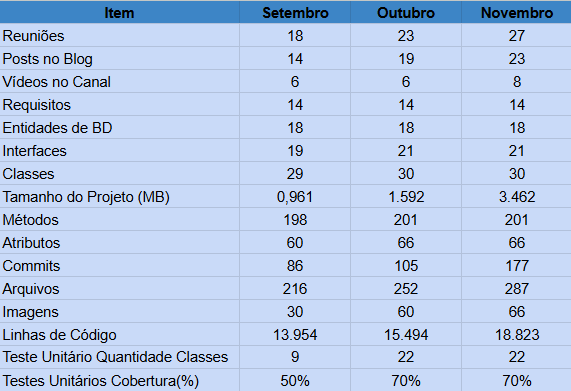
\includegraphics[width=0.85\textwidth]{images/tabela-metricas.png}
        \caption{Tabela de métricas do projeto primeiro semestre 2024}
        \label{fig:enter-label}
    \end{figure}
As métricas representam numericamente o andamento do projeto, demonstrando quais foram os períodos de maior atividade do grupo e o tamanho do projeto como um todo.

\newpage

\subsection{Ferramentas Auxiliares}

Com o intuito de simplificar o processo de análise do projeto como um todo, foi usada a ferramenta MetricRunner, que auxilia na contagem do número de classes, interfaces, métodos, atributos, arquivos e linhas de código do projeto Vocco.
Para fazer uso desta ferramenta é necessário cumprir os seguintes passos: 

1- Buscar no Maven Central a Biblioteca Reflections versão 0.9.9-RC1;

2- Adicionar a dependência da biblioteca indicada, no arquivo Pom;

3- Adicionar a classe MetricRunner à aplicação;

4- Alterar o valor da variável rootPackage para o nome do pacote raiz da aplicação;  

5- Executar a classe MetricRunner.


\subsection{Estatísticas do Projeto}

Para obtenção de elementos visuais, e mais informações estatísticas à respeito de ambos os projetos (\textit{back-end} e \textit{front-end}), foi utilizada a ferramenta GitStats para a geração de gráficos e tabelas informativas.


Na figura \ref{fig:dadosGeraisRepositorioBack}, são apresentados os dados gerais à respeito do repositório GitHub referente ao projeto \textit{back-end}.

\begin{figure}[ht]
        \centering
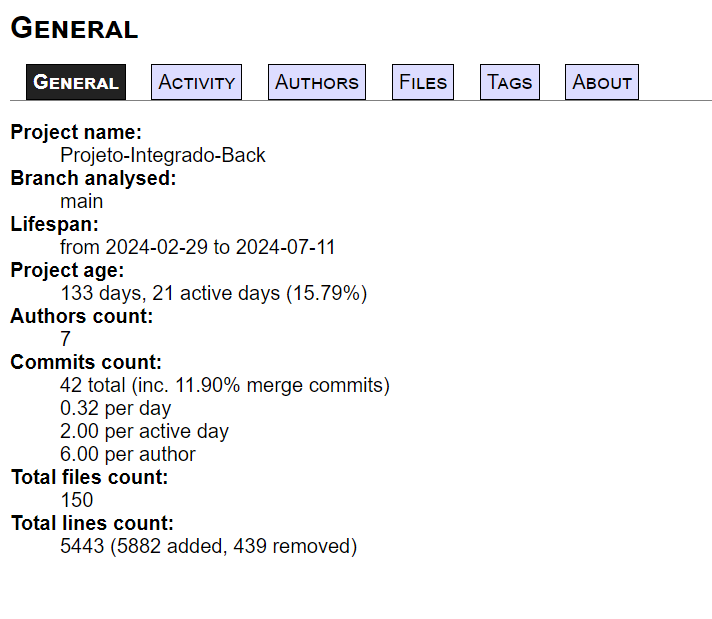
\includegraphics[width=0.65\textwidth]{images/dados-gerais-stats-back.png}
        \caption{Dados Gerais sobre o repositório \textit{back-end} do GitHub}
        \label{fig:dadosGeraisRepositorioBack}
    \end{figure}

\newpage

Na figura \ref{fig:dadosCommitsDiasBack} são apresentados os dados referentes à relação entre o dia da semana, e o horário em que foram feitos os commits no repositório do projeto \textit{back-end} do GitHub.

\begin{figure}[ht]
        \centering
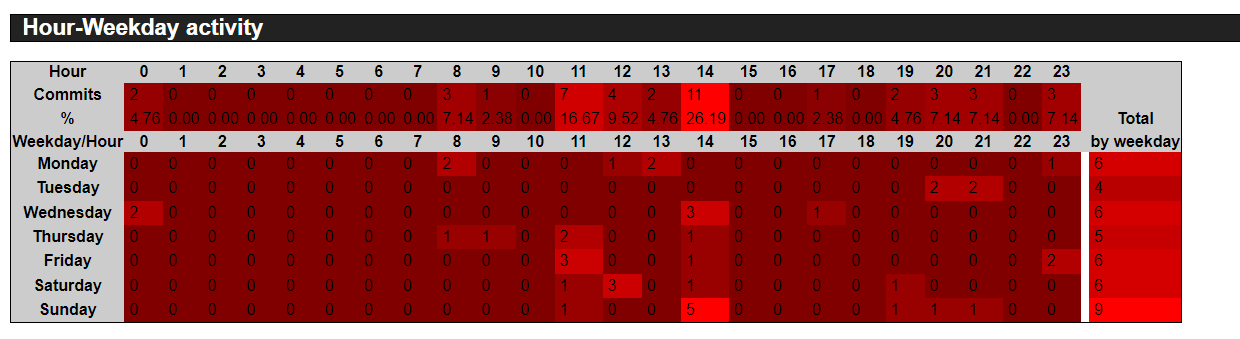
\includegraphics[width=1.0\textwidth]{images/commits-hora-semana-stats-back.png}
        \caption{Dados Gerais sobre o repositório \textit{back-end} do GitHub}
        \label{fig:dadosCommitsDiasBack}
    \end{figure}

Na figura \ref{fig:commitsBack} são apresentados os dados referentes ao número de commits em cada mês do ano de 2024 referente ao repositório do projeto \textit{back-end} do GitHub.

\begin{figure}[ht]
        \centering
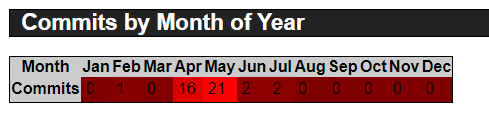
\includegraphics[width=0.75\textwidth]{images/commits-mes-stats-back.png}
        \caption{Número de commits em cada mês do ano de 2024}
        \label{fig:commitsBack}
    \end{figure}
    

Na figura \ref{fig:commitsAutorBack} são apresentados os dados referentes ao número de commits por autor no repositório do projeto \textit{back-end} do GitHub.  

\begin{figure}[ht]
        \centering
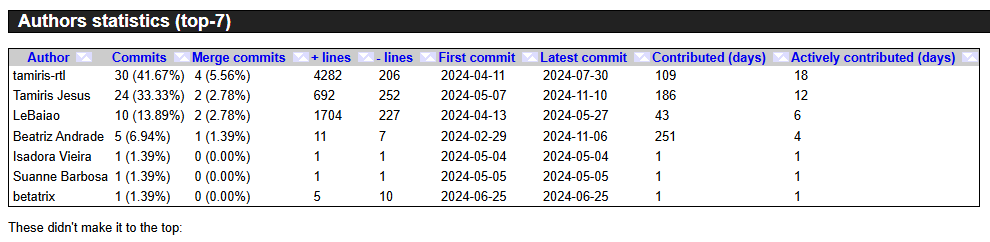
\includegraphics[width=1.0\textwidth]{images/autores-stats-back.png}
        \caption{Número de commits por autor}
        \label{fig:commitsAutorBack}
    \end{figure}

\newpage

Na figura \ref{fig:numeroLinhasBack} é apresentado o gráfico referente ao número de linhas de código adicionadas por autor no repositório do projeto \textit{back-end} do GitHub.  

\begin{figure}[ht]
        \centering
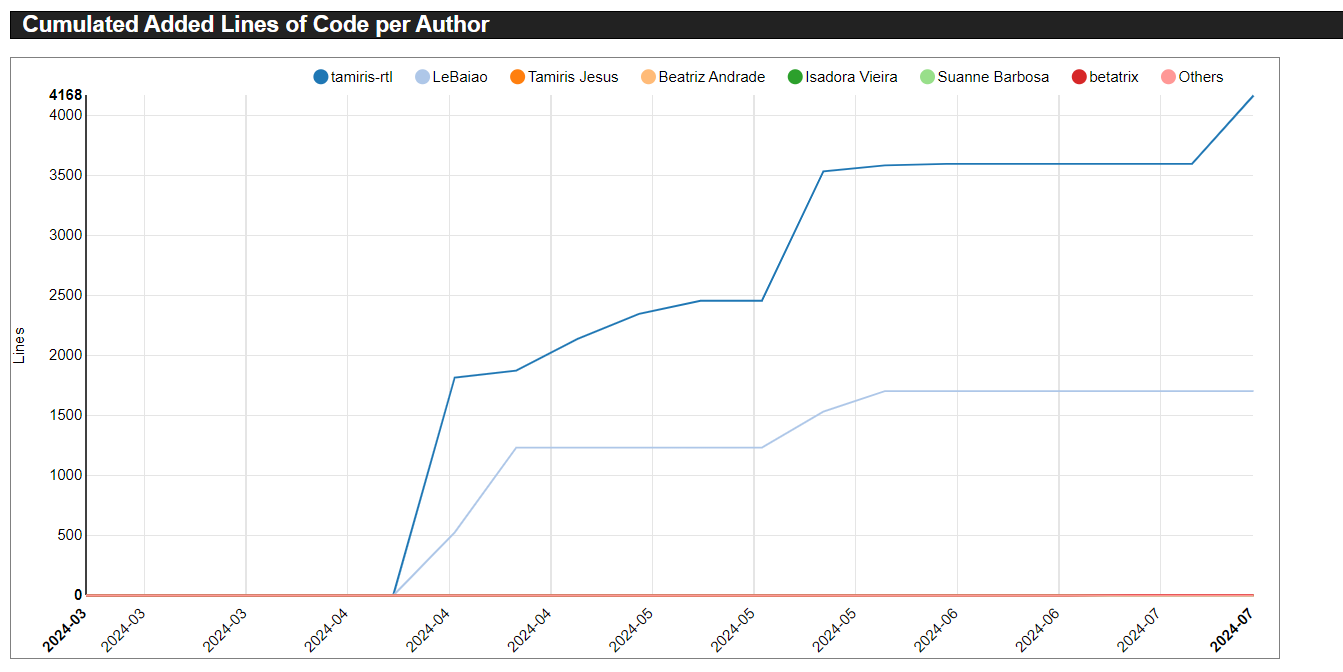
\includegraphics[width=1.0\textwidth]{images/linhas-por-autor-stats-back.png}
        \caption{Número de linhas de código por autor}
        \label{fig:numeroLinhasBack}
    \end{figure}



Na figura \ref{fig:linhasPorAutorBack} é apresentado o gráfico referente ao número de commits por autor no repositório do projeto \textit{back-end} do GitHub.  

\begin{figure}[ht]
        \centering
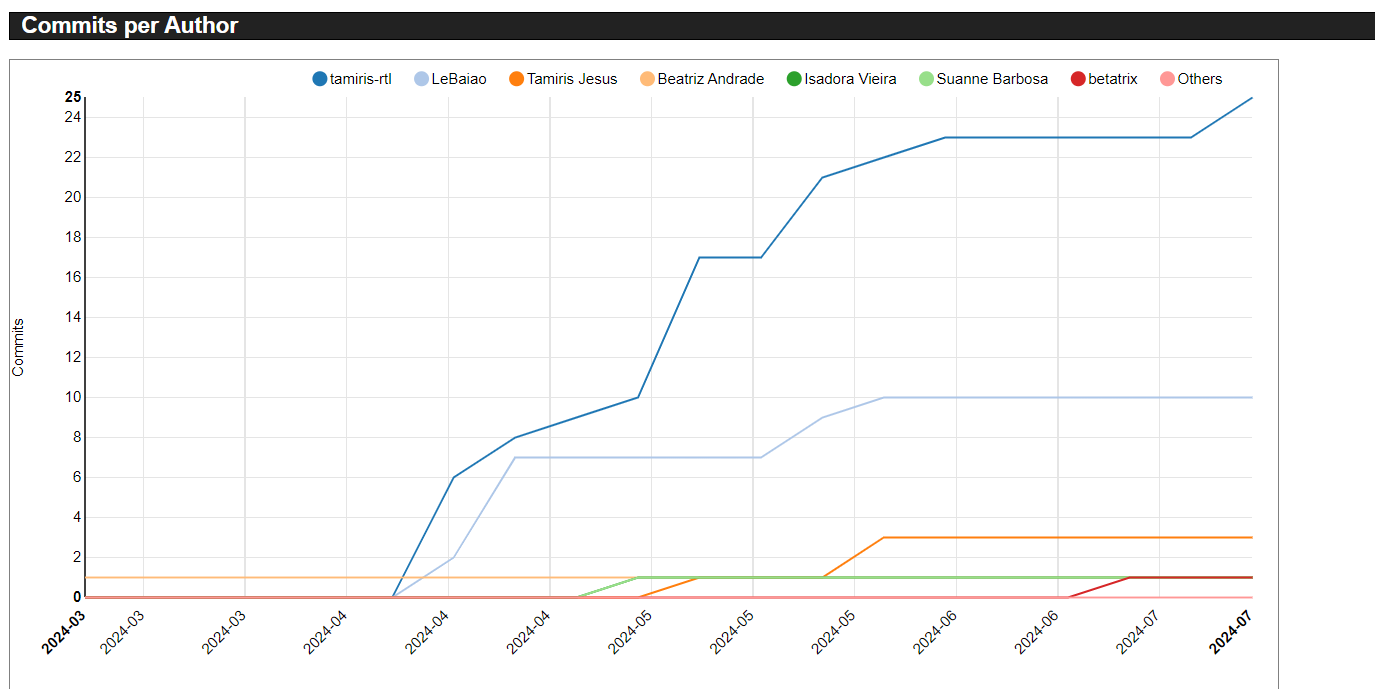
\includegraphics[width=1.0\textwidth]{images/commits-autor-stats-back.png}
        \caption{Gráfico número de commits por autor}
        \label{fig:linhasPorAutorBack}
    \end{figure}

\newpage

A figura \ref{fig:linhasPorAutor2Back} é um complemento do gráfico da figura 19, no qual é apresentado o gráfico referente ao número de commits por autor no repositório do projeto \textit{back-end} do GitHub.  

\begin{figure}[ht]
        \centering
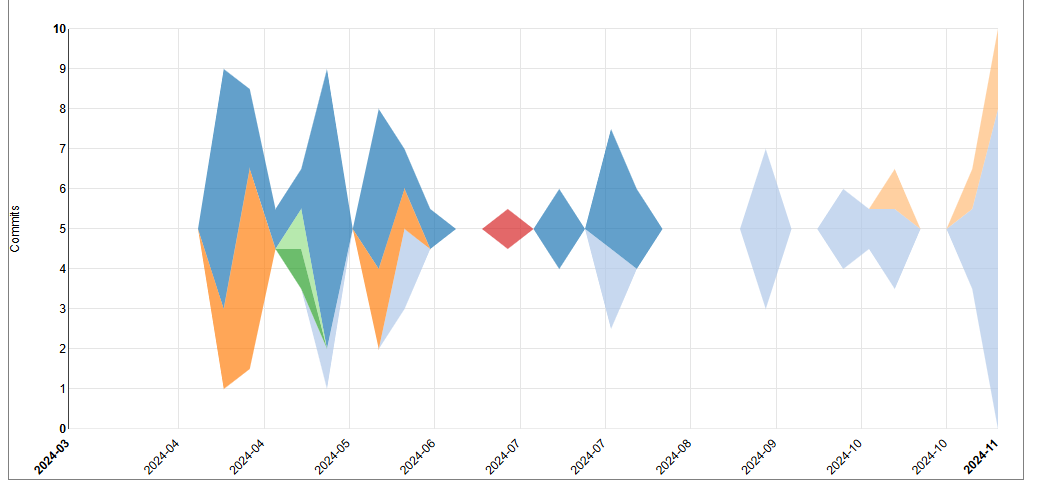
\includegraphics[width=1.0\textwidth]{images/commits-autor2-stats-back.png}
        \caption{Gráfico número de commits por autor}
        \label{fig:linhasPorAutor2Back}
    \end{figure}



Na figura \ref{fig:rankingAutoresBack} é apresentado o ranking dos autores com o maior número de commits em cada mês do ano de 2024 no repositório do projeto \textit{back-end} do GitHub.

\begin{figure}[ht]
        \centering
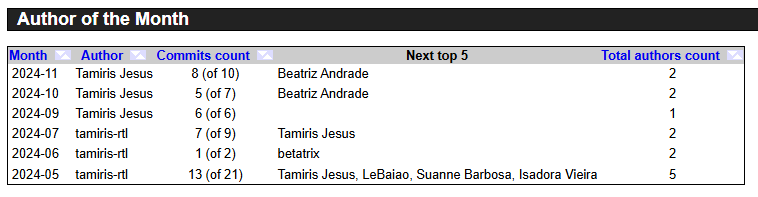
\includegraphics[width=1.0\textwidth]{images/rank-autor-stats-back.png}
        \caption{Tabela autor com o maior número de commits em cada mês do ano de 2024}
        \label{fig:rankingAutoresBack}
    \end{figure}

\newpage

Na figura \ref{fig:arquivosPorDataBack} é apresentado o gráfico referente ao número de arquivos adicionados e número de linhas de código no repositório do projeto \textit{back-end} do GitHub no decorrer do primeiro semestre de 2024.

\begin{figure}[ht]
        \centering
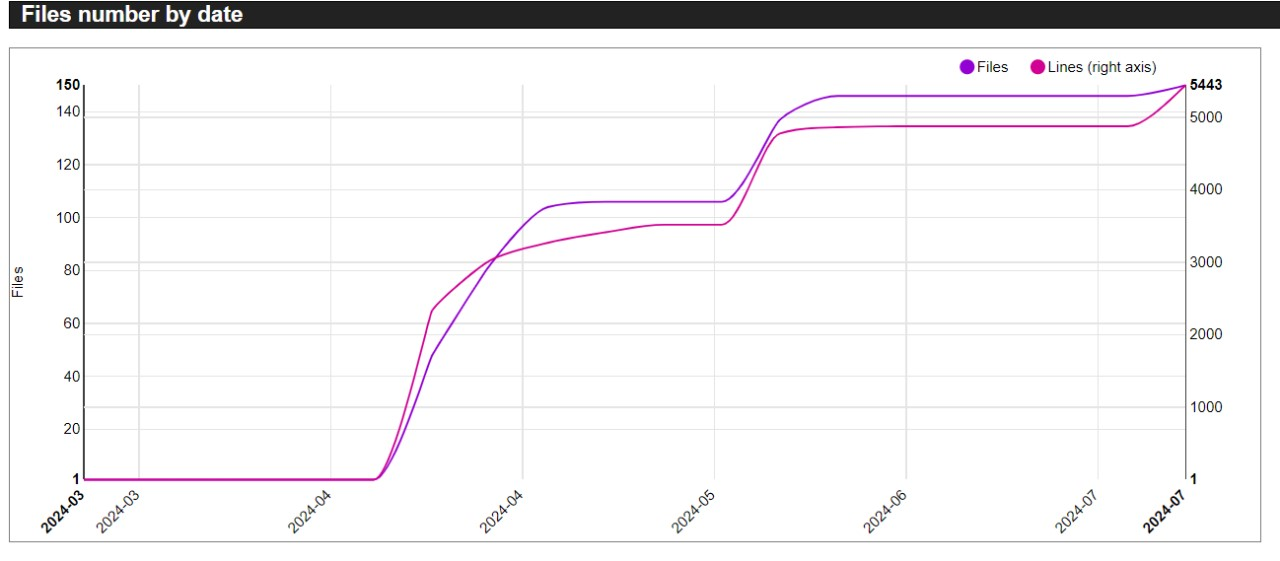
\includegraphics[width=1.0\textwidth]{images/arquivos-por-data-stats-back.jpg}
        \caption{Gráfico com a relação número de arquivos adicionados e linhas de código}
        \label{fig:arquivosPorDataBack}
    \end{figure}


Na figura \ref{fig:tiposdeArquivosBack} são apresentados os dados referentes ao tipo de arquivo presente no projeto \textit{back-end}.

\begin{figure}[ht]
        \centering
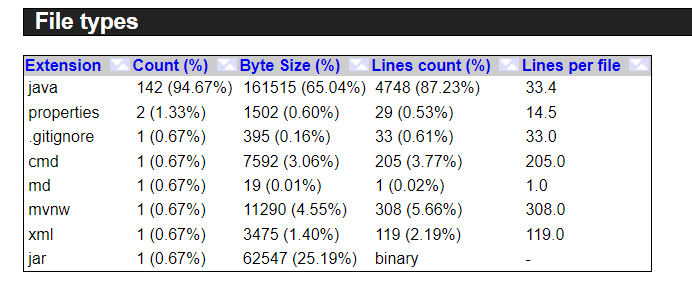
\includegraphics[width=1.0\textwidth]{images/tipos-arquivos-stats-back.png}
        \caption{Tipos de arquivos presentes no repositório do projeto \textit{back-end} do GitHub}
        \label{fig:tiposdeArquivosBack}
    \end{figure}

\newpage

Na figura \ref{fig:infoArquivosBack} são apresentados os dados gerais referente aos arquivos presentes no projeto \textit{back-end}.

    \begin{figure}[ht]
        \centering
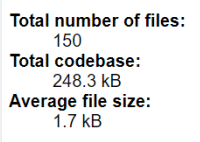
\includegraphics[width=0.5\textwidth]{images/info-arquivos-stats-back.png}
        \caption{Dados de arquivos presentes no repositório do projeto \textit{back-end}}
        \label{fig:infoArquivosBack}
    \end{figure}


Na figura \ref{fig:dadosGeraisFront}, são apresentados os dados gerais à respeito do repositório GitHub referente ao projeto \textit{front-end}.

\begin{figure}[ht]
        \centering
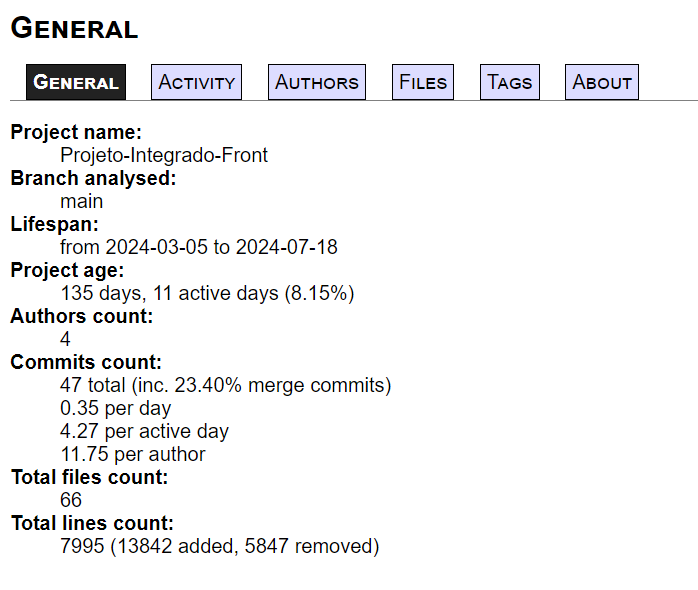
\includegraphics[width=0.65\textwidth]{images/dados-gerais-stats-front.png}
        \caption{Dados Gerais sobre o repositório \textit{front-end} do GitHub}
        \label{fig:dadosGeraisFront}
    \end{figure}

\newpage


Na figura \ref{fig:commitsPorHoraFront} são apresentados os dados referentes à relação entre o dia da semana, e o horário em que foram feitos os commits no repositório do projeto \textit{front-end} do GitHub.

\begin{figure}[ht]
        \centering
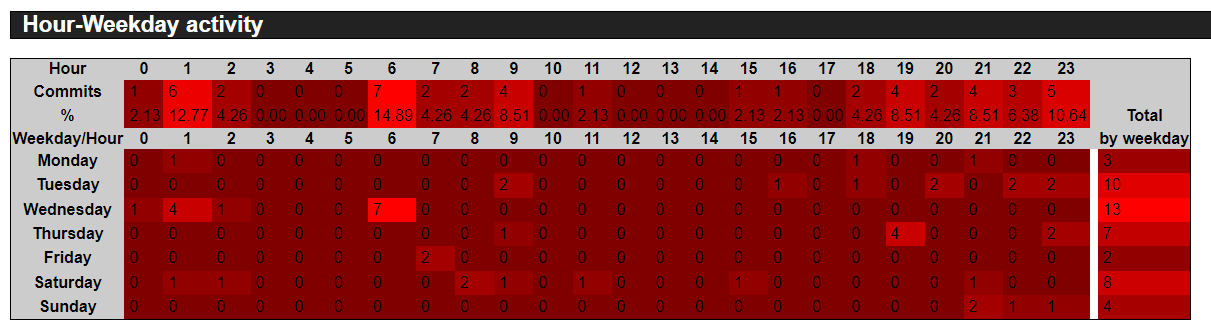
\includegraphics[width=1.0\textwidth]{images/commits-hora-semana-stats-front.png}
        \caption{Dados Gerais sobre o repositório \textit{front-end} do GitHub}
        \label{fig:commitsPorHoraFront}
    \end{figure}

Na figura \ref{fig:commitsPorMesFront} são apresentados os dados referentes ao número de commits em cada mês do ano de 2024 referente ao repositório do projeto \textit{front-end} do GitHub.

\begin{figure}[ht]
        \centering
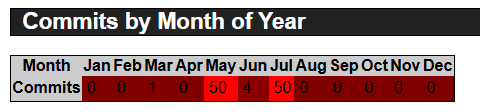
\includegraphics[width=0.75\textwidth]{images/commits-mes-stats-front.png}
        \caption{Número de commits em cada mês do ano de 2024}
        \label{fig:commitsPorMesFront}
    \end{figure}

Na figura \ref{fig:commitsPorAutorFront} são apresentados os dados referentes ao número de commits por autor no repositório do projeto \textit{front-end} do GitHub.  

\begin{figure}[ht]
        \centering
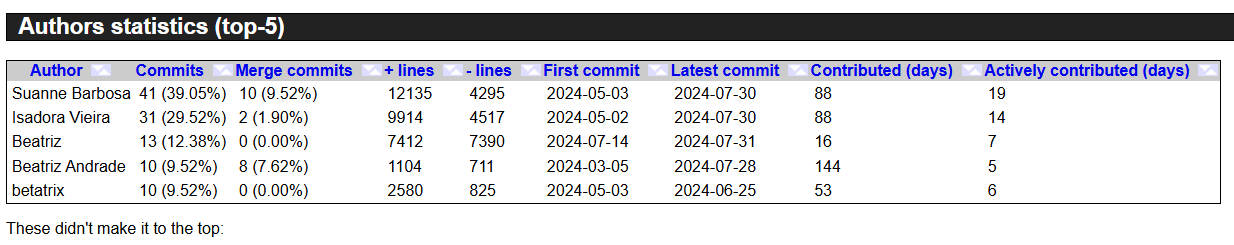
\includegraphics[width=1.0\textwidth]{images/autor-stats-front.png}
        \caption{Número de commits por autor}
        \label{fig:commitsPorAutorFront}
    \end{figure}

\newpage

Na figura \ref{fig:linhasPorAutorFront} é apresentado o gráfico referente ao número de linhas de código adicionadas por autor no repositório do projeto \textit{front-end} do GitHub.  

\begin{figure}[ht]
        \centering
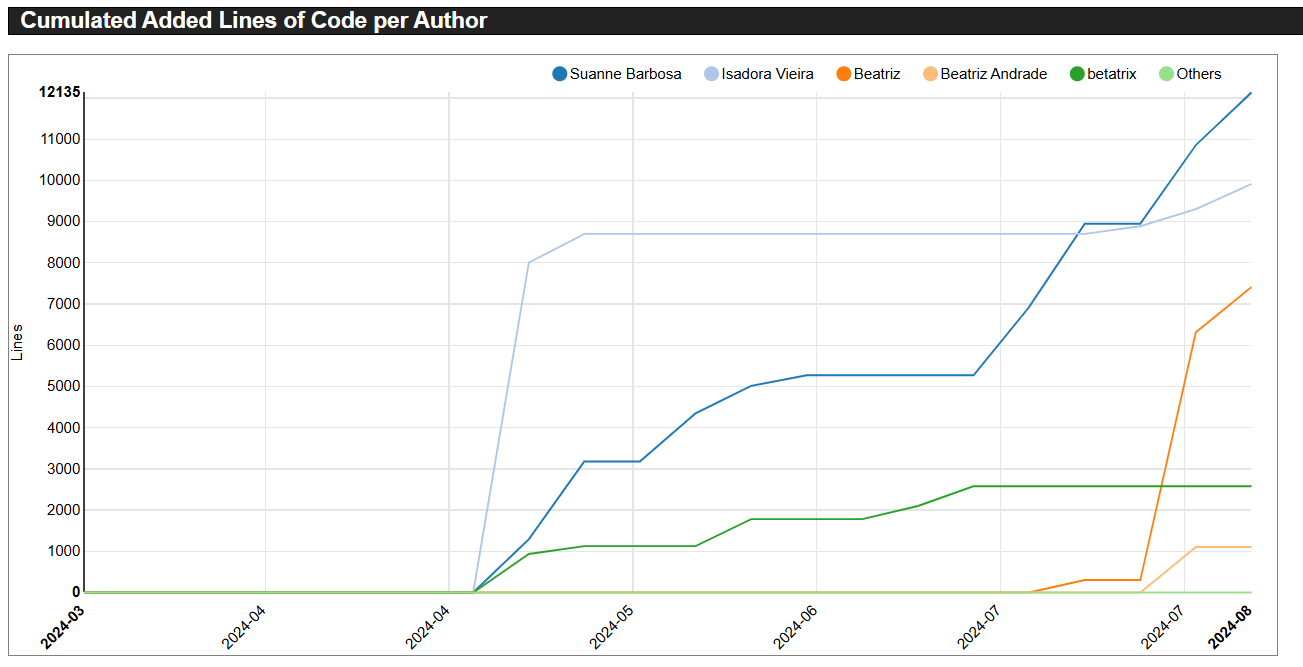
\includegraphics[width=1.0\textwidth]{images/linhas-por-autor-stats-front.png}
        \caption{Número de linhas de código por autor}
        \label{fig:linhasPorAutorFront}
    \end{figure}


Na figura \ref{fig:graficoCommitsPorAutorFront} é apresentado o gráfico referente ao número de commits por autor no repositório do projeto \textit{front-end} do GitHub.  

\begin{figure}[ht]
        \centering
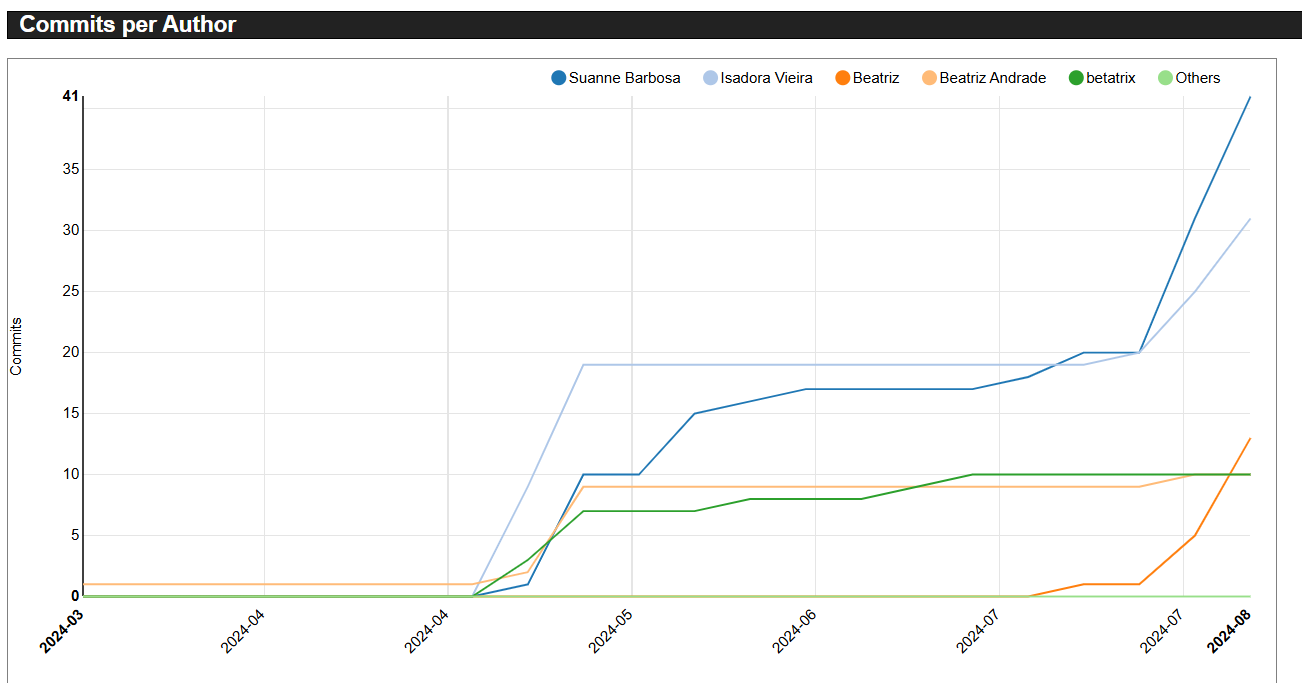
\includegraphics[width=1.0\textwidth]{images/commits-autor-stats-front.png}
        \caption{Gráfico número de commits por autor}
        \label{fig:graficoCommitsPorAutorFront}
    \end{figure}

\newpage

A figura \ref{fig:graficoCommitsPorAutorFront2} é um complemento do gráfico da figura 30, no qual é apresentado o gráfico referente ao número de commits por autor no repositório do projeto \textit{front-end} do GitHub.  

\begin{figure}[ht]
        \centering
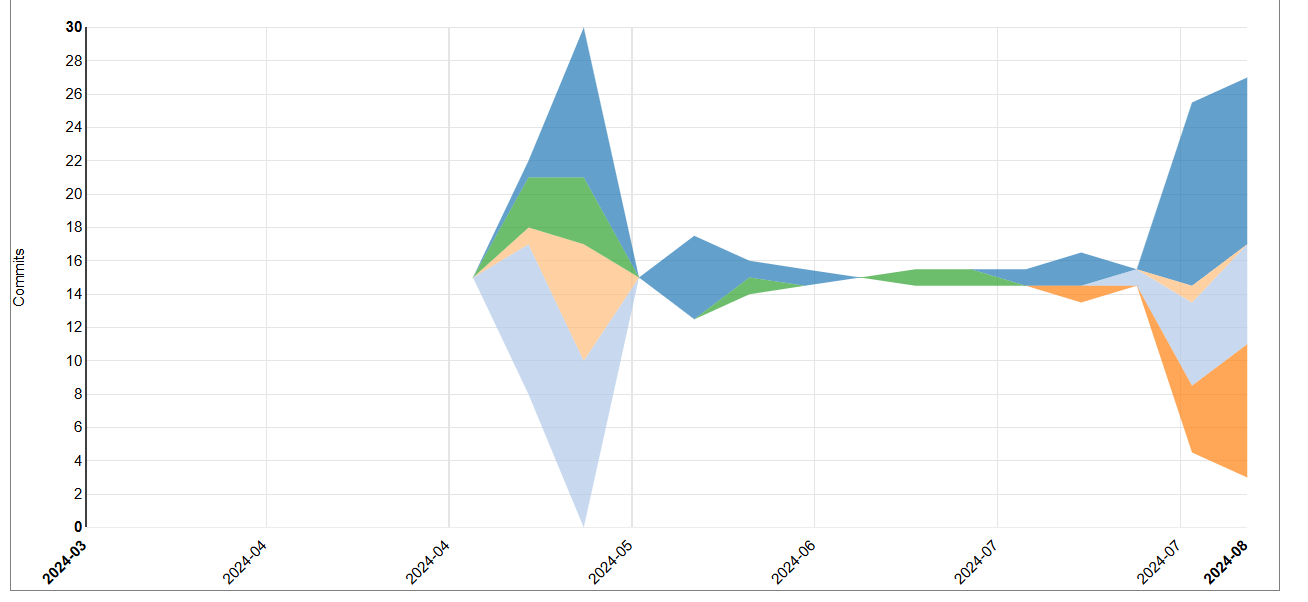
\includegraphics[width=1.0\textwidth]{images/commits-autor2-stats-front.png}
        \caption{Gráfico número de commits por autor}
        \label{fig:graficoCommitsPorAutorFront2}
    \end{figure}


Na figura \ref{fig:rankingAutoresFront} é apresentado o ranking dos autores com o maior número de commits em cada mês do ano de 2024 no repositório do projeto \textit{front-end} do GitHub.  

\begin{figure}[ht]
        \centering
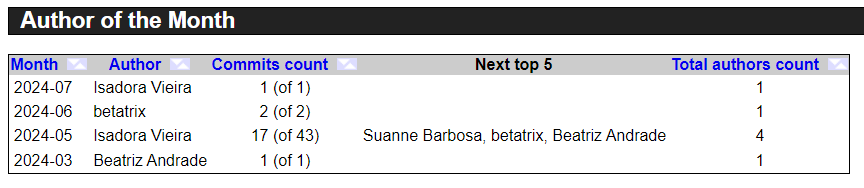
\includegraphics[width=1.0\textwidth]{images/rank-autor-stats-front.png}
        \caption{Tabela autor com o maior número de commits em cada mês do ano de 2024}
        \label{fig:rankingAutoresFront}
    \end{figure}

\newpage

Na figura \ref{fig:numeroLinhasFront} é apresentado o gráfico referente ao número de arquivos adicionados e número de linhas de código no repositório do projeto \textit{front-end} do GitHub no decorrer do primeiro semestre de 2024.

\begin{figure}[ht]
        \centering
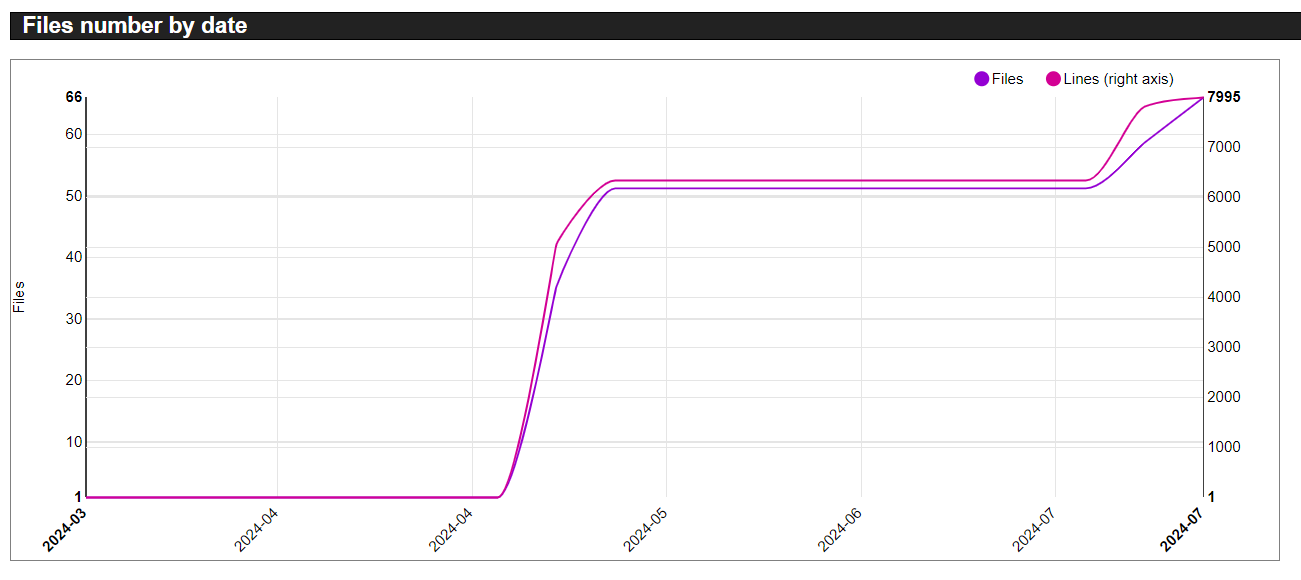
\includegraphics[width=1.0\textwidth]{images/arquivos-por-data-stats-front.png}
        \caption{Gráfico com a relação número de arquivos adicionados e linhas de código}
        \label{fig:numeroLinhasFront}
    \end{figure}

Na figura \ref{fig:tiposdeArquivosFront} são apresentados os dados referentes ao tipo de arquivo presente no projeto \textit{front-end}.

\begin{figure}[ht]
        \centering
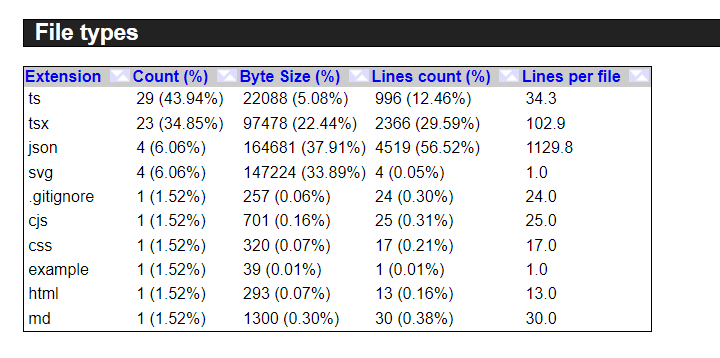
\includegraphics[width=1.0\textwidth]{images/tipos-arquivos-stats-front.png}
        \caption{Tipos de arquivos presentes no repositório do projeto \textit{front-end} do GitHub}
        \label{fig:tiposdeArquivosFront}
    \end{figure}

\newpage


Na figura \ref{fig:infoArquivosFront} são apresentados os dados gerais referente aos arquivos presentes no projeto \textit{front-end}.

    \begin{figure}[ht]
        \centering
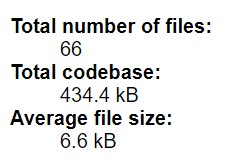
\includegraphics[width=0.5\textwidth]{images/info-arquivos-stats-front.jpg}
        \caption{Dados de arquivos presentes no repositório do projeto \textit{front-end}}
        \label{fig:infoArquivosFront}
    \end{figure}


Com esses dados estatísticos à respeito dos repositórios do projeto Vocco, é possível obter uma visão ampla da evolução desenvolvimento e como a participação de cada integrante do grupo é essencial, auxiliando na construção do sistema como um todo.

% % \chapter{Informações sobre as atividades desenvolvidas}

% Esse capitulo apresenta as atividades a serem desenvolvidas durante o projeto, as seções em sua maioria seguem a ordem de desenvolvimento. Mas algumas atividades podem acontecer paralelamente a outras, e em alguns casos a preparação para o desenvolvimento da atividade deve ser feito antecipadamente.

% \section{Definição da equipe}\label{atv-definicao-equipe}
% Os alunos devem se organizar em equipes de acordo com o número definido pelos professores no primeiro dia de aula. Normalmente as equipes variam entre 4 e 6 participantes de acordo com o número de alunos em cada turma. 

% \todo[inline]{Aqui a definição do gerente e escolha das equipes seria o ideal, mas nunca aceitam fazer, se tiverem alguma sugestão é interessante colocar}

% \todo[inline]{Muitos casos escolhem os amigos e quando um realmente assume o papel de gerente depois deixam de ser amigos.... Quando não estão preocupados vão levando de qualquer forma}

% \todo[inline]{a escolha do perfil dos participantes é importante, mas normalmente só escolhem os amigos}



% \section{Planejamento do projeto}\label{atv-planejamento-projeto}

% Para se obter o resultado desejado e chegar ao objetivo é importante um planejamento adequado e um acompanhamento da evolução desse plano para chegar ao objetivo. Algumas  atividades devem ser executadas de forma sequencial e portanto o planejamento correto evita atrasos pois não adianta colocar mais energia/pessoas para reduzir o tempo de determinadas atividades ou executar paralelamente \cite{brooks1995mythical}.
% % Nine people can’t make a baby in a month. (regarding the addition of more programmers to get a project completed faster)



% \section{Escolha do(a) gerente da equipe}\label{atv-escolha-gerente}
% Cada equipe deve definir um Gerente que deve ser responsável por organizar durante todo o período de desenvolvimento do projeto. O Gerente também é responsável por participar das reuniões de gerencia que podem acontecer durante a disciplina, onde os professores podem passar informações para as equipes.


% \section{Envio da linha correspondente ao acessos.txt}\label{atv-acessos}
% Para a criação do diretório correspondente da equipe no repositório de controle de versão \atividade{controle-de-versao}, cada equipe deve enviar para os professores uma linha de texto simples (por e-mail) no mesmo formato do arquivo \textbf{acessos.txt} disponível na raiz do repositório de controle de versão. Os prontuários utilizados nesse arquivo devem ser definidos em letras minúsculas, e o acesso ao repositório sempre deve ser feito com login em letras minúsculas.

% A maior parte das atividades da disciplina depende do acesso a este repositório, sendo importante que essa atividade seja cumprida no menor tempo para garantir o acesso de todos ao repositório.


% \section{Criação de canal no YouTube}\label{atv-criacao-youtube}
% Deve ser criado um canal no YouTube para publicação de todos os vídeos gerados durante o desenvolvimento e apresentações do projeto.

% \begin{itemize}
%     \item todos os vídeos publicados devem ter na descrição e nas tags \textbf{\acs{ifsp}}, \textbf{\acs{spo}} e \textbf{\codigoDisciplina};
    
%     \item vídeos do \gls{gource} devem ser publicados nesse canal \autoref{atv-video-gource}.
% \end{itemize}

% \section{Criação de blog}\label{atv-criacao-blog}
% Deve ser criado um blog para a equipe com as seguintes características:
% \begin{itemize}
%     \item Deve ter um feed \acs{rss} ou Atom, de forma a permitir que as publicações sejam visualizadas na íntegra em ferramentas de consumo destes formatos;
    
%     \item O modelo utilizado para o blog deve ser tal que permita a visualização completa de cada publicação, sem necessidade de clicar em um \enquote{ver mais} ou um ícone para permitir a visualização.
    
% \end{itemize}

% A partir da criação do blog, toda semana deverá ser feita uma publicação de acordo com o descrito na \autoref{atv-publicacao-blog}

% A lista de blogs de projetos anteriores está disponível em: \dicasIvan{blogs-de-trabalhos}, muitos desses blogs possuem relatos e dicas que podem auxiliar no desenvolvimento do seu projeto.


% \section{Criação e atualização do arquivo equipe.yaml}\label{atv-equipe-yaml}
% Deve ser criado um arquivo no diretório da equipe, no repositório de controle de versão, com as informações sobre a equipe e o projeto que vai ser desenvolvido. Esse arquivo deve ser criado a partir da definição da equipe (\autoref{atv-definicao-equipe}) e deverá ser atualizado se houverem mudanças nas informações (ex a primeira versão do arquivo não possui detalhes sobre o projeto a ser desenvolvido, quando o projeto for aprovado pelos professores então o arquivo deverá ser atualizado).

% O arquivo deve seguir o mesmo formato dos arquivos já existentes nos diretórios de equipes de projetos anteriores e ser validado com a ferramenta yamllint \url{https://github.com/adrienverge/yamllint} que é utilizada no servidor. Outras ferramentas que possuem o mesmo nome podem ter critérios diferentes de validação então é importante a utilização da ferramenta sugerida.
% \justificativa{Muitos alunos tentam utilizar um site com esse nome que não valida da mesma forma e o arquivo acaba sendo recusado.  }

% Esse arquivo é a base para definição da página \dicasIvan{blogs-de-trabalhos}, caso a sua equipe não apareça nessa listagem provavelmente o seu arquivo é invalido, e na página existe um link para ver o arquivo combinado que contem as mensagens de erro de validação.

% Esses arquivos são processados diariamente para atualização no site.






% \section{Documentos do projeto}\label{documentos-latex}

% Todos os documentos que serão entregues para avaliação devem ser feitos utilizando o \LaTeX \space de acordo com os padrões da \ac{abnt} e do Guia de Normatização do \ac{ifsp}. Um modelo de documento está disponível em \urlmodelo \space e contem exemplos de diversos itens que normalmente são utilizados nesses documentos. O documento modelo também possui informações sobre procedimentos para revisão dos textos.


% No repositório de controle de versão existem documentos de outras equipes que também podem ser utilizados como referência. O documento de modelo também possui informações sobre o desenvolvimento de software e problemas encontrados em projetos anteriores tanto em documentação como em relação ao desenvolvimento. 

% Na página \dicasIvan{textos} existem diversas informações uteis para facilitar a elaboração do seu documento. Cuidado com plágio \dicasIvan{plagio}, não faça cópias de outros documentos, escreva com suas palavras e referencie a informação.

% A ferramenta overleaf onde o modelo de documento se encontra é uma ferramenta de desenvolvimento de textos \LaTeX, que possui algumas limitações na versão gratuita, é importante que os alunos mantenham um ambiente de compilação em seus computadores de forma a não ficarem dependentes dessa ferramenta \emph{online}. Algumas atividades como a criação do documento de diferenças entre versões \atividade{latexdiff} dependem de um ambiente corretamente configurado e que não funciona diretamente no overleaf. Alguns professores já possuem contas com características adicionais da conta gratuita do overleaf e podem compartilhar projetos com mais recursos, mas isso não deve ser considerado como a solução normal de uso da equipe.
% \justificativa{Aqui é importante que aqueles que não tem os recursos ainda compartilhem os seus links de referencia do overleaf para ganharem esse tipo de acesso, acho que são somente 10 referencias para ganhar histórico e compartilhamento ilimitado}


% \section{Utilização do repositório de controle de versão}
% \label{atv-controle-de-versao}
% \todo{Aqui precisa de ajuste para as disciplinas do superior que podem utilizar repositório externo e precisam sincronizar a cada 15 dias}
% É obrigatório o uso do repositório de controle de versão indicado pelos professores. A \ac{url} para acesso é disponibilizada no moodle da disciplina. O acesso deve ser feito utilizando como login o prontuário do aluno (spXXXXXX) sempre em letras minusculas. A senha é a mesma que é utilizada para acesso na rede sem fio do Campus e pode ser redefinida no site \url{https://central.spo.ifsp.edu.br/}. O repositório é um sistema de controle de versão centralizado Subversion (informações adicionais em \dicasIvan{subversion}).

% O uso correto do repositório permite o desenvolvimento pelos diversos membros da equipe de forma remota mantendo o conteúdo em local de fácil acesso para todos. Os \glspl{commit} devem ser frequentes para garantir que todos tenham acesso ao desenvolvimento atual da equipe, devem seguir as regras indicadas no arquivo \textbf{txt} na raiz do repositório. Cada equipe também deve manter seu próprio \gls{backup} dos dados do repositório.

% Cada \gls{commit} deve ter um comentário descrevendo que que foi alterado, essa informação é muito importante também para criação posterior do vídeo com a ferramenta \gls{gource} \atividade{video-gource}.

% O Código e documentação de projetos anteriores do curso técnico e superior fica disponível para consulta por todos os alunos do Campus São Paulo do \ac{ifsp}.

% A cada entrega/apresentação deve ser feita uma \emph{tag} no repositório indicando a data e tipo de entrega (ex. 2020-02-10-Prova-de-Conceito)\footnote{ \emph{tag} é uma função disponível em sistemas de controle de versão, não significa criar um diretório com o nome indicado}.

% Se o projeto a ser desenvolvido for um desenvolvimento de funções adicionais para projeto de código aberto, será permitida a utilização de um repositório externo público após a avaliação e aprovação dos professores. O repositório oficial do \ac{ifsp} deverá ser ser sincronizado pelo menos uma vez a cada 15 dias com a versão atualizada do repositório externo.

% \justificativa{No técnico que ainda não tem experiencia continuamos com o repositório centralizado}





% \section{Escolha da metodologia de gerenciamento}\label{atv-metodologia-gerenciamento}

% Cada equipe tem liberdade para escolha das metodologias utilizadas durante o projeto, para o controle do projeto deve ser escolhida uma (ou combinação de metodologias) de forma a gerenciar a evolução das atividades. É importante que a equipe realmente siga a metodologia escolhida e utilize os artefatos da metodologia.

% \section{Escolha da metodologia de desenvolvimento}\label{atv-metodologia-desenvolvimento}

% Cada equipe tem liberdade para escolha das metodologias utilizadas durante o desenvolvimento, para o desenvolvimento do software deve ser escolhida uma (ou combinação de metodologias) de forma executar o desenvolvimento. É importante que a equipe realmente siga a metodologia escolhida e utilize os artefatos da metodologia.

% \section{Estudo de tecnologias}\label{atv-estudo-tecnologias}

% Antes de iniciar o projeto deve ser feito um estudo das tecnologias que podem ser aplicadas no projeto, pequenos programas de teste podem ser desenvolvidos nesse momento para verificar a aderência dessa tecnologia aos objetivos do projeto. Tecnologias já conhecidas reduzem os estudos, mas deve-se tomar cuidado pois existem casos onde mesmo com um novo aprendizado outras tecnologias podem ser mais eficientes para o projeto.

% É importante considerar também os custos de determinadas tecnologias ou plataformas. Se o objetivo do projeto é criar uma solução para uma entidade sem fins lucrativos e que não tenha verbas para manter um sistema no ar, não vai adiantar escolher uma plataforma que tenha um custo mensal.
% Além disso algumas plataformas tecnologias possuem limites que podem não ser suficientes para o desenvolvimento da aplicação.

% O \ac{ifsp} possui convênios que permitem acesso a pacotes de serviços de forma gratuita e também existem programas gratuitos dos grandes provedores de nuvem (ex AWS Educate).
% Analisando projetos anteriores \atividade{avaliacao-projetos-anteriores} é possível obter um grande conjunto de ideias sobre tecnologias possíveis de utilização. 



% \section{Definição de tecnologias}\label{atv-definicao-tecnologias}

% Após o estudo das tecnologias passiveis de aplicação no projeto a equipe deve fazer suas escolhas e desenhar o projeto de acordo com as tecnologias estudadas.
% Em alguns casos os provedores de nuvem permitem escolher onde a aplicação será hospedada, Brasil, Europa, América do Norte etc dependendo do tipo de aplicação a localização pode afetar a latência e a experiencia do usuário. 

% As escolhas devem ser justificadas e compatíveis com os objetivos do projeto.
% \melhorar{complementar mais aqui....}


% \section{Proposta inicial}\label{atv-proposta-inicial}
% Cada equipe deve elaborar uma proposta indicando a aplicação que deseja desenvolver, a proposta deve ser desenvolvida e apresentada para a turma. Os professores tem que aprovar o tema e o escopo do projeto a ser desenvolvido. É importante que as aulas anteriores sejam utilizadas para apresentar e negociar com os professores as possíveis propostas de forma que, no dia da apresentação, já seja apresentada a versão final acordada com os os professores.


% \begin{itemize}

%     \item A ordem de apresentação é definida por sorteio;
    
%     \item Documento \ac{pdf} gerado no \LaTeX, com aproximadamente 5 páginas de texto contendo contextualização, ideia, objetivos, análise de concorrentes, referências utilizadas a partir da análise de projetos anteriores \atividade{avaliacao-projetos-anteriores} e indicação de tecnologias que pretendem utilizar \atividade{estudo-tecnologias};
    
%     \item \emph{Slides} para apresentação da proposta inicial \atividade{slides};
    
%     \item Uma apresentação de 10 minutos devera ser feita e será seguida de perguntas/comentários dos professores e alunos da turma;

%     \item Vídeo de 5 minutos no YouTube demonstrando essa proposta \atividade{criacao-youtube};
    
%     \item Auto avaliação da equipe \atividade{planilha-notas} deve ser entregue no repositório.
% \end{itemize}



% \section{Definição de coding convention}\label{atv-coding-convention}

% A equipe deve definir o padrão de codificação que ira utilizar e seguir durante todo o desenvolvimento de forma que todo o código siga um padrão único. Existem ferramentas de \gls{analise-estatica} que também verificam se o formato do código segue um padrão pré-definido, a utilização dessas ferramentas ajuda a seguir esse requisito de desenvolvimento. 

% \section{Modelagem de dados}\label{atv-modelagem-dados}
% A modelagem de dados é fundamental para o correto funcionamento de um software. Sendo assim, é importante que a equipe efetue a modelagem correta seguindo o método pertinente ao seu projeto (seja pela utilização de um \ac{mer}, seja pela utilização de um diagrama de classes, quando utilizado um \ac{orm}). Ainda, não basta que seja feita a modelagem, mas que se olhe de forma criteriosa para o modelo gerado e que ele seja validado com dados reais pertinentes à solução proposta.

% Uma forma simples de verificar se um determinado modelo de dados atente é fazer exercícios simples de inserção, atualização e exclusão considerando os cenários da aplicação, usando ferramentas simples, como planilhas, e, com base nas informações registradas, tentar \enquote{responder}  a consultas que serão relevantes para seus usuários (observando os requisitos do projeto), de forma a ver se a informação correta será obtida como resposta (e fazendo os devidos ajustes no modelo caso contrário).


% \melhorar{falar sobre dados históricos / temporais, eles esquecem coisas básicas como preço que deve ser registrado em uma compra para no futuro saber o valor}

% \section{Codificação da aplicação}\label{atv-codificacao-aplicacao}

% Durante o desenvolvimento da aplicação diversos critérios devem ser seguidos para garantir que o seu código seja claro tanto para os programadores como para os computadores, os computadores entendem qualquer código que siga os critérios de sintaxe definidos da linguagem, mas as pessoas podem ter dificuldade, a utilização de um mesmo padrão por toda a equipe facilita \atividade{coding-convention}, além da utilização de padrões já existentes de estruturas de dados e de codificação. Isso facilita tanto a manutenção por outras pessoas como também pelo próprio desenvolvedor.

% Tenham em mente as seguintes frases\footnote{\url{https://www.javacodegeeks.com/2012/11/20-kick-ass-programming-quotes.html}}:
% \begin{itemize}

% % https://groups.google.com/g/comp.lang.c++/c/rYCO5yn4lXw/m/oITtSkZOtoUJ?pli=1
%     \item \enquote{Always code as if the guy who ends up maintaining your code will be a violent psychopath who knows where you live.} – Martin Golding;
    
%     \item \enquote{Any fool can write code that a computer can understand. Good programmers write code that humans can understand.} – Martin Fowler;
    
%     \item \enquote{Good code is its own best documentation. As you’re about to add a comment, ask yourself, \textquote{How can I improve the code so that this comment isn’t needed?}} – Steve McConnell.
    
% \end{itemize}

% \todo[inline]{Buscar as referencias originais}
% \todo[inline]{também é um bom local para colocar mais informações do Clean Code}

% \section{Criação de ambiente para aplicação}\label{atv-criacao-ambiente}
% A partir das escolhas feitas pela equipe \atividade{definicao-tecnologias} deve ser criado o ambiente no provedor escolhido para a aplicação. O ambiente para desenvolvimento e apresentação pode ser uma versão reduzida do ambiente necessário para a aplicação (ex em produção a aplicação precisa de Balanceador de Carga mas para desenvolvimento isso não é necessário). Além disso o ambiente pode ser criado em localização diferente da ideal para redução de custos.
% Diferenças entre o ambiente proposto para execução da aplicação e o ambiente utilizado devem ser claramente detalhadas na documentação.
% Considerando que os serviços gratuitos possuem limites é possível a utilização de servidores distribuídos entre contas dos membros da equipe. Além disso é importante tomar o cuidado com serviços que fazem cobrança após o limite gratuito de forma a não terem despesas desnecessárias.



% \section{Disponibilização da aplicação na internet}\label{atv-hostname}
% Para que a aplicação fique disponível na internet deverá ser utilizado um nome de acesso \emph{hostname} em vez de endereço IP. Isso garante que mesmo na mudança do local de hospedagem o endereço de acesso permanece inalterado. Poderá ser utilizado um serviço de \ac{dns} dinâmico (dyndns), endereço oferecido pelo provedor de serviço ou um domínio registrado caso a equipe tenha interesse posterior em manter a aplicação (mas não é necessário o registro de domínio próprio para cumprir os requisitos da disciplina)



% \section{Prova de conceito}\label{atv-prova-de-conceito}
% Deverá ser desenvolvida uma Prova de Conceito (\ac{poc}) que deve demonstrar a aderência das tecnologias escolhidas com a aplicação que deve ser desenvolvida. Essa prova de conceito deve demonstrar a comunicação desde o usuário até a base de dados e utilizar de forma simples as tecnologias escolhidas para demonstrar que elas funcionam para o objetivo desejado.
% \todo[inline]{Alguns não entenderam claramente o que deve entrar na POC, precisamos desenhar melhor....}

% \begin{itemize}
%     \item Deve ficar disponível de forma pública na internet;
    
%     \item Utilizar os ambientes/plataformas escolhidos para implantação \atividade{criacao-ambiente};
    
%     \item Comunicação criptografada \atividade{https};
    
%     \item Demonstrar o funcionamento da internacionalização (duas línguas), utilizando corretamente as funcionalidades da linguagem a partir de arquivos de recursos com as definições textuais de cada linguagem (não deve ser utilizada tradução de página via Google tradutor);
    
%     \item Demonstrar que os dados do usuário são enviados para o servidor e armazenados na base de dados;
    
%     \item Demonstrar que APIs especificas atendem as necessidades desejadas;
    
%     \item Auto avaliação da equipe \atividade{planilha-notas};
    
%     \item Um vídeo de aproximadamente 3 minutos demonstrando a aderência desta prova de conceito com a aplicação final \atividade{criacao-youtube};
    
%     \item Um relatório (máximo de 5 páginas) identificando as tecnologias utilizadas e como elas serão utilizadas no projeto (diagrama de arquitetura);
    
%     \item Vídeo do \gls{gource} \atividade{video-gource};
    
%     \item Uma apresentação de 15 minutos para professores e alunos;

%     \item \emph{Slides} \atividade{slides};

%     \item A ordem de apresentação é definida por sorteio.
    
    
% \end{itemize}

% \section{Apresentação parcial}\label{atv-apresentacao-parcial}
% A apresentação parcial consiste em mostrar a situação atual do projeto para os professores e alunos das outras equipes, é importante a utilização de um roteiro para demonstrar de maneira eficiente a situação em que o desenvolvimento se encontra tanto em termos de aplicação como de documentação.

% \begin{itemize}

%     \item Auto avaliação da equipe \atividade{planilha-notas};
    
%     \item Vídeo do \gls{gource} \atividade{video-gource};
    
%     \item Uma apresentação de 20 minutos para professores e alunos;

%     \item \emph{Slides} \atividade{slides};

%     \item A ordem de apresentação é definida por sorteio.
    
% \end{itemize}





% \section{Vídeo do gource}\label{atv-video-gource}
% O video criado com a representação do desenvolvimento no controle de versão deve ser feito com a ferramenta \gls{gource} e deve considerar os seguintes itens:

% \begin{itemize}
%     \item Utilizar opção \textbf{\emph{--key}};
    
%     \item Utilizar as opções de legendas (\textbf{\emph{caption}}) para registrar as principais mudanças feitas no repositório;
    
%     \item Deve ter aproximadamente 1 minuto para cada bimestre de desenvolvimento;
    
%     \item Alterar os \textbf{\emph{userid}} do repositório pelos nomes dos participantes;
    
%     \item Colocar uma imagem distinta e especifica para cada usuário;
    
%     \item Deve ser publicado no canal do YouTube \atividade{criacao-youtube}.
% \end{itemize}

% A cada entrega de aplicação e no final de cada bimestre deve ser criado um novo vídeo do \gls{gource}.



% \section{Publicação semanal no blog}\label{atv-publicacao-blog}

% O blog tem por objetivo servir como registro das atividades realizadas pela equipe a ser acompanhado pelos docentes. Também é importante como memória da equipe, permitindo a consulta pelos membros da equipe de forma a verificar o que ocorreu em uma determinada semana. Dessa forma, é importante considerar o relato do que realmente ocorreu (inclusive pode-se utilizar a publicação combinada a artefatos da metodologia de gerenciamento de projetos utilizada).

% A cada semana deve ser publicado no blog pelo menos uma vez indicando as atividades desenvolvidas por cada elemento da equipe. Deve indicar claramente quem foi a pessoa que fez a publicação.

% As publicações semanais no blog devem conter um relatório gerencial de andamento do projeto, com identificação do desempenho e das tarefas individuais (ex. reuniões de \emph{milestones}, \emph{project checkpoint}, \emph{sprint review} etc.).


% \section{Comunicação criptografada utilizando \acs{https}/\acs{tls}}\label{atv-https}
% A comunicação entre os  módulos da aplicação  e usuário devem sempre ser feitas de forma segura. Para isso deve ser utilizado o protocolo \ac{https} ou \ac{tls} que permitem a comunicação de forma criptografada. A configuração pode ser feita utilizando um certificado gratuito como o disponibilizado pelo serviço Let's Encrypt ou também utilizando serviços gratuitos como CloudFare, CloudFront etc.

% A configuração desse serviço deve ser avaliada e obter uma nota mínima \textbf{A} \autoref{atv-ssllabs}

% \section{Avaliação da configuração \acs{https}/\acs{tls}}\label{atv-ssllabs}

% É importante garantir a confidencialidade entre o usuário e a aplicação no servidor, para isso deve ser utilizado um protocolo de criptografia, o mais utilizado é o \ac{https} que pode ser configurado com um certificado gratuito como Let's Encrypt, AWS ou similar ou através de um serviço que já ofereça esse acesso criptografado (CloudFront, Cloudflare etc). O processo de criptografia deverá ser documentado e a configuração deverá ser analisada utilizando a ferramenta \url{https://www.ssllabs.com/ssltest/} onde deve obter no mínimo a nota A (existem poucos casos onde pode aceita uma nota inferior, mas esses casos devem ser negociados com os professores).




% \section{Avaliação de respostas HTTP}\label{atv-security-headers}
% Para maior segurança da aplicação e dos usuários existem diversos cabeçalhos que podem ser configurados nas respostas do protocolo \ac{http}, para validação desses cabeçalhos deverá ser utilizada a ferramenta de análise disponível em \url{https://securityheaders.io/}, dependendo do tipo de aplicação as condições podem variar e portanto deverá ter a melhor nota possível nessa ferramenta justificando os resultados na documentação.

% \section{Análise estática}\label{atv-analise-estatica}
% O processo de \gls{analise-estatica} permite avaliar o código fonte da aplicação sem necessidade de execução dos programas por meio de testes \atividade{testes}. É uma atividade incremental que deve ser executada de forma constante de forma a evitar problemas no código. Desenvolver o código de forma limpa e sem erros conhecidos reduz o retrabalho e facilita para todos os membros da equipe.

% \section{Documentação via \gls{openapi}}\label{atv-openapi}

% A definição dos pontos de chamadas da aplicação deve ser feita utilizando o padrão \gls{openapi} (padrão que foi definido a partir da ferramenta Swagger). Com a integração de diversas aplicações via protocolo \ac{http} foi criado um padrão \gls{openapi} que permite a definição de forma padronizada de como os "serviços" da aplicação podem ser executados. Isso facilita também a troca de interfaces da aplicação de uma maneira muito simples e também os testes da aplicação. Apesar de existirem ferramentas especificas para chamadas \ac{http} a definição utilizando um padrão permite a migração entre essas ferramentas de forma transparente. 

% A documentação deve ser publicada juntamente com a aplicação e somente os pontos principais indicados no documento.


% \section{Sistema de log}\label{atv-log}
% A aplicação deverá ser desenvolvida utilizando um ou mais sistema de Log de forma a organizar o registro da aplicação e permitir a configuração do armazenamento de acordo com a plataforma de implantação. A utilização de uma biblioteca já existente facilita no código e também para o administrador. Existem diversas bibliotecas que podem ser utilizadas como: commons-logging, log4j, slf4j, log4php, log4net, logcat etc.


% \section{Testes}\label{atv-testes}
% Testes garantem que a aplicação atenda os requisitos definidos durante o seu desenvolvimento. É importante que os testes sejam executados repetidamente e de forma padronizada para isso é necessário que seja criado um Plano de testes para execução manual e também a criação de testes automatizados de forma a reduzir a carga de trabalho e evitar erros. Os testes devem considerar tanto os casos de sucesso como de erro, não adianta testar somente as condições principais de uso, pois durante o uso normal dados errados serão colocados pelo usuário e essas condições deverão ser verificadas também.





% \section{Testes automatizados}\label{atv-testes-automatizados}

% Os testes automatizados evitam o trabalho manual repetitivo e garantem a maior confiabilidade do sistema. Qualquer um pode e deve executar esses testes sempre que uma nova versão for gerada garantindo que a aplicação esteja se comportando da maneira projetada. Esses testes podem iniciar com testes unitários (que verificam um método/função) e ir até testes complexos de integração onde a aplicação é executada em ambiente de execução de forma a garantir que esteja funcionando corretamente. Para isso devem ser utilizadas ferramentas especificas de automatização de testes pois elas já simplificam esse processo.




% \section{Documento com diferenças - latexdiff}\label{atv-latexdiff}
% De forma a demonstrar facilmente as alterações feitas entre duas versões de um documento, deverá ser utilizada a ferramenta \gls{latexdiff} para criação de um documento que demonstra essas diferenças. Cada vez que um documento atualizado for entregue deve ser gerado o \gls{latexdiff} demonstrando as diferenças para a versão anterior. Por isso é muito importante salvar no repositório de controle de versão a revisão utilizada em cada entrega.

% Apesar de existirem algumas versões disponíveis na internet para esse tipo de comparação o documento deve ser gerado localmente em seus computadores, o processo é muito simples mas depende da preparação do ambiente, por isso é importante a preparação antes da data de entrega do documento. O comando recomendado para execução do \gls{latexdiff} pode ser encontrado em \dicasIvan{latexdiff}.




% \section{Planilha de auto avaliação da equipes}\label{atv-planilha-notas}
% Em cada entrega e apresentação cada equipe deverá preencher uma planilha de avaliação onde cada elemento deve dar uma nota, e justificar, para cada elemento da equipe, inclusive a sua própria nota. A planilha de modelo está disponível em \dicasIvan{projetos-e-apresentacoes}. Essa planilha deverá ser salva em um arquivo \ac{pdf} contendo todas as abas originais da planilha e em uma boa formatação para fácil leitura e análise.


% \justificativa{Muitas vezes eles mandam imprimir sem ajustar as páginas e fica tudo quebrado e difícil de ler}





% \section{Entrega da primeira versão do projeto}\label{atv-primeira-versao}

% Seguindo o plano de aulas do \ac{suap} deverá ser entregue no repositório de controle de versão a documentação do projeto.
% \justificativa{Pelo menos uma pois existem casos onde por causa dos feriados e sincronização entre as turmas acabamos tendo que colocar mais de uma semana. 2021 estamos fazendo isso}

% \begin{itemize}
%     \item Documento \ac{pdf} gerado no \LaTeX, com relatório do desenvolvimento \atividade{relatorio-do-desenvolvimento};
% \end{itemize}

% \section{Apresentação da primeira versão do projeto}\label{atv-apresentacao-primeira-versao}

% Cada equipe deve apresentar para a banca examinadora e alunos da turma. Todas equipes devem observar e analisar as apresentações das outras equipes pois devem fazer um relatório avaliando cada outra equipe (Documentos, Apresentação e Aplicação) \atividade{relatorio-analise-projetos}

% É importante lembrar que o(s) convidado(s) não participaram do processo vão avaliar o trabalho e portanto sem conhecimento prévio do que é a aplicação ou do que foi o desenvolvimento.

% \begin{itemize}

%     \item Slides para apresentação  \atividade{slides};
    
%     \item A apresentação deve ter duração de no máximo 45 minutos, seguida de perguntas dos professores;
    
%     \item Pelo menos 15 minutos do tempo da apresentação deve ser reservado para demonstração da aplicação desenvolvida \atividade{demonstracao-aplicacao};
    
%     \item Vídeo de 10 minutos no YouTube demonstrando a aplicação desenvolvida \atividade{criacao-youtube};
    
%     \item Vídeo do \gls{gource} \atividade{video-gource};
    
%     \item Auto avaliação da equipe \atividade{planilha-notas}.
% \end{itemize}


% \section{Relatório do desenvolvimento}\label{atv-relatorio-do-desenvolvimento}

% O relatório deve seguir o padrão \ac{abnt} no formato disponibilizado, deve conter:

% \begin{itemize}
%     \item Introdução;
    
%     \item Problema a ser solucionado;
    
%     \item Justificativa;
    
%     \item Objetivos do projeto;
    
%     \item Revisão da literatura com os assuntos tratados no trabalho:
%         \begin{itemize}
%             \item Não misturar o desenvolvimento feito pela equipe com os estudos feitos;
            
%             \item Não incluir pesquisa sobre temas das disciplinas do curso, somente temas relacionados ao domínio do problema a ser solucionado;
%         \end{itemize}
        
%     \item Histórico das atividades, incluindo informações sobre a gestão do projeto;
    
%     \item Reuniões;
    
%     \item Desenvolvimentos de código, dados;
    
%     \item Levantamentos;

%     \item Escolhas;
    
%     \item Descartes (mudanças de rumo durante o projeto);

%     \item Problemas ocorridos no desenvolvimento / gerenciamento;
    
%     \item Protocolos;
    
%     \item Modelos de dados, classes, índices de banco de dados etc \atividade{modelagem-dados};
    
%     \item Contribuições efetuadas aos projetos de código aberto utilizados;
    
%     \item Tabela com evolução das métricas do projeto \atividade{tabela-metricas};
    
%     \item informações estatísticas do repositório de controle de versão \atividade{estatisticas-repositorio};
    
%     \item Links do projeto:
%     \begin{itemize}
%         \item Controle de versão;
        
%         \item Vídeos;
        
%         \item Blog;
        
%         \item Aplicação web se for publicada na internet;
        
%         \item etc.
%     \end{itemize}
    
%     \item Anexos / Apêndices: 
%     \begin{itemize}
%         \item Todas as publicações semanais do blog \atividade{criacao-blog};
        
%         \item Documento de aprovação \atividade{proposta-inicial}

%         \item Documento da prova de conceito \atividade{prova-de-conceito}

%         \item Cronogramas;
        
%         \item Planos de teste;
        
%         \item Análise de cobertura dos testes;
        
%         \item Relatório análise estática \atividade{analise-estatica};
        
%         \item Manual de usuário \atividade{manual-usuario};
        
%         \item Manual de técnico \atividade{manual-tecnico}.
        
%     \end{itemize}
% \end{itemize}

% Todos os dados qualitativos e quantitativos sobre o projeto (métricas, estatísticas, análises) devem ser efetivamente coerentes com a realidade.

% Elementos como as publicações do blog devem ser apresentados na ordem cronológica de publicação.



% \section{Tabela com evolução das métricas do projeto}\label{atv-tabela-metricas}

% Para demonstrar a evolução do projeto deverá ser criada uma tabela para demonstrar a evolução das métricas do projeto. Essas métricas devem ser registradas pelo menos uma vez por mês. Caso o projeto tenha módulos distintos (servidor, cliente etc) essa tabela deverá ser separada tendo uma tabela para cada módulo e também tabela com totais. A tabela também poderá ser dividida para facilitar a visualização em tabelas com itens de desenvolvimento, gerenciamento, etc.

% Elementos que devem constar:
% \begin{itemize}
%     \item Reuniões;
    
%     \item Publicações de blog;
    
%     \item Requisitos;
    
%     \item Tamanho do projeto;
    
%     \item Arquivos;
    
%     \item Linhas;

%     \item Classes;
    
%     \item Interfaces;
    
%     \item Métodos;
    
%     \item Atributos;
    
%     \item Testes \atividade{testes}
    
%     \item Testes unitários / automatizados \atividade{testes-automatizados}
%     \begin{itemize}
%         \item Classes de testes;
        
%         \item Quantidade de testes;
        
%         \item Percentual de cobertura;
        
%     \end{itemize}
    
%     \item Dados sobre análise estática \atividade{analise-estatica};
    
%     \item \glspl{commit} \atividade{controle-de-versao};
    
%     \item Entidades de banco de dados;
    
%     \item Imagens;
    
%     \item Sons;
    
%     \item Vídeos gerados;
    
%     \item Outros elementos pertinentes para o projeto ou gerenciamento.
% \end{itemize}


% \section{Informações de utilização do repositório}\label{atv-estatisticas-repositorio}

% Para demonstrar a utilização do repositório de controle de versão devem ser apresentadas informações estatísticas geradas pela ferramenta StatSVN. Os dados devem ser comentados. Alguns gráficos são obrigatórios:
%     \begin{itemize}
%         \item Todos commits por autor \waUrl{https://statsvn.org/statsvn/commitscatterauthors.png};
        
%         \item Atividade por autor \waUrl{http://statsvn.org/statsvn/activity.png};
        
%         \item Atividade por dia da semana
%         \waUrl{http://statsvn.org/statsvn/activity\_day.png};
        
%         \item Atividade por hora do dia \waUrl{http://statsvn.org/statsvn/activity\_time.png}.
%     \end{itemize}

% Antes de gerar os gráficos os logs do repositório devem ser ajustados de forma a indicar claramente qual foi a pessoa que fez as atividades e não somente o login das pessoas. Dependendo da versão utilizada de subversion existe um bug que já foi detectado e que pode ser contornado facilmente (informações em \dicasIvan{subversion}).
%     \todo[inline]{Talvez colocar colocar as imagens do statsvn aqui no documento}




% \section{Manual de usuário}\label{atv-manual-usuario}
% Para que o usuário possa utilizar o sistema deverá ser criado um ou mais manuais de usuário (de acordo com possíveis perfis de usuário na aplicação). É bem claro que determinadas aplicações devem ser executadas sem que o usuário tenha que ler um manual, algumas aplicações tem que ter uma interface muito simples para que o usuário não precise ler o manual e para alguns outros casos pequenos vídeos de introdução ou tutoriais dentro da aplicação podem ser suficientes. Existem casos onde é necessário um manual especifico para administrados, moderador etc. A determinação da necessidade do manual escrito ou não deve ser negociada individualmente entre cada equipe e os professores/clientes.


% \section{Manual técnico}\label{atv-manual-tecnico}

% O Manual técnico é aquele que permite que desenvolvedores possam fazer manutenções e atualizações no sistema e o administrador de sistemas possa fazer a implantação, configuração, backup e gerenciamento geral. Esse documento pode fazer parte do relatório geral do desenvolvimento ou ser um documento separado. Caso a equipe opte por um manual separado é importante organizar as informações de forma a não ficar repetindo entre os documentos.



% \section{Demonstração da aplicação desenvolvida}\label{atv-demonstracao-aplicacao}

% Para demonstrar o desenvolvimento a aplicação deve ser apresentada em funcionamento, é importante que seja definido um roteiro para demonstrar as principais funcionalidades e processos da aplicação, a aplicação deve ser populada previamente com dados suficientes para demonstrar o seu funcionamento e entendimento correto, os dados tem que ser compatíveis com o objetivo da aplicação. 

% Durante uma apresentação com tempo limitado pontos básicos de cadastro devem ser limitados a demonstrar alguns elementos e validações, os processos e funções que a aplicação faz para resolver problemas dos usuários devem ser o foco.

% Em alguns casos (como por exemplo utilização de \ac{gps}) alguns recursos não podem ser apresentados em tempo real e portando podem ser apresentados por meio de vídeos gravados com antecedência.






% \section{Slides}\label{atv-slides}
% Para apresentações devem ser gerados \emph{slides} que tem que ser entregues também no repositório de controle de versão. Esses \emph{slides} devem possuir numeração e podem seguir o modelo que está disponível em \urlmodeloApresentacao \space esse modelo foi desenvolvido também com \LaTeX \space de forma que todos os elementos utilizados na documentação podem ser reaproveitados. Apesar dos \emph{slides} serem um roteiro a seguir durante as apresentações é importante que antes da apresentação seja feito um treino para verificar a sequencia e o tempo da apresentação são compatíveis com o solicitado. Todos \emph{slides} que forem utilizados nas apresentações também devem ser colocados em formato \ac{pdf} no repositório.

% A sua apresentação será vista por pessoas que não participaram do desenvolvimento, é importante a contextualização/introdução do que será apresentado. 




% ----------------------------------------------------------
% Finaliza a parte no bookmark do PDF
% para que se inicie o bookmark na raiz
% e adiciona espaço de parte no Sumário
% ----------------------------------------------------------
\phantompart

% ----------------------------------------------------------
% ELEMENTOS PÓS-TEXTUAIS
% ----------------------------------------------------------
\postextual
% ----------------------------------------------------------

% ----------------------------------------------------------
% Referências bibliográficas
% ----------------------------------------------------------
\bibliography{referencias}
% ----------------------------------------------------------
% Glossário
% ----------------------------------------------------------
%
%
\ifdef{\printnoidxglossary}{
    \addcontentsline{toc}{chapter}{GLOSSÁRIO}
    \printnoidxglossary[style=glossario]
    %\printglossaries
}{}


%% ----------------------------------------------------------
% Apêndices
% Documentos gerados pelo próprio autor
% ----------------------------------------------------------

% ---
% Inicia os apêndices
% ---
\begin{apendicesenv}

% Imprime uma página indicando o início dos apêndices
\partapendices

\chapter{PROTOTIPAÇÃO}
\label{apendice_a}

\section{Tela Inicial do administrador}
\begin{figure}[H]
    \centering
    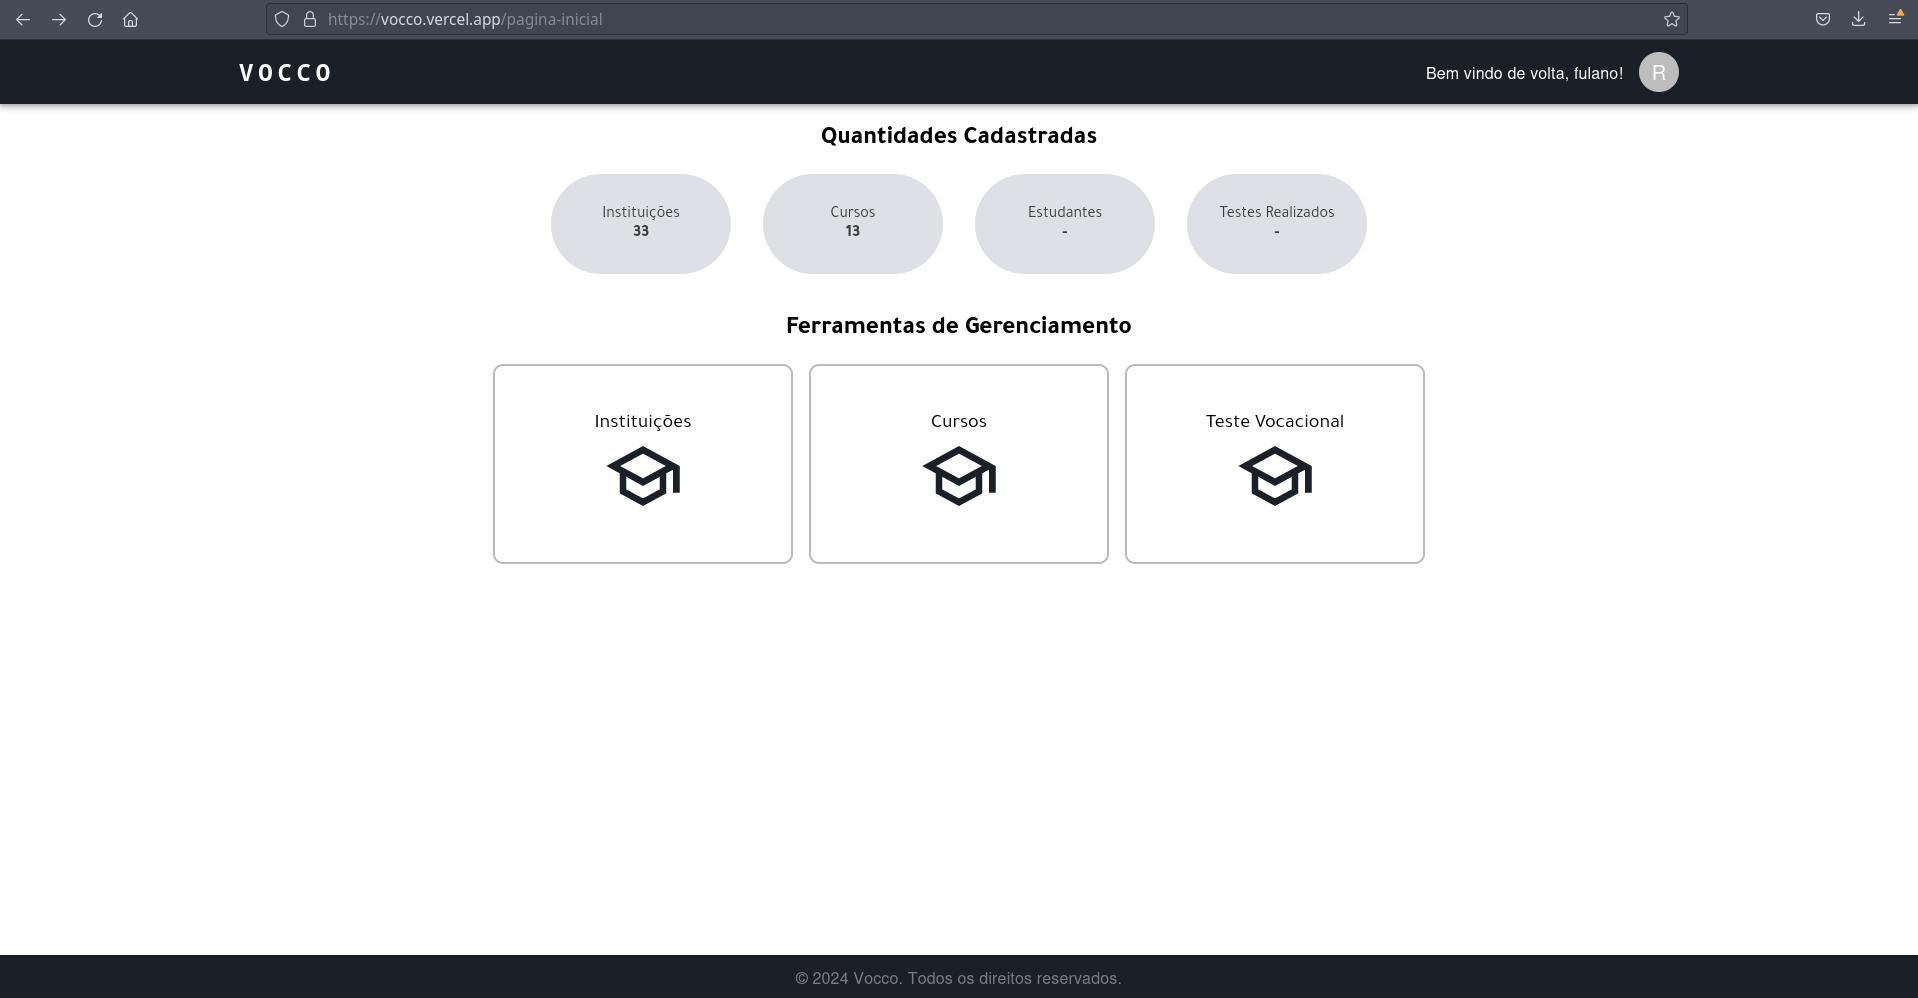
\includegraphics[width=1.0\linewidth]{images/telaInicial.png}
    \caption{Tela inicial do administrador}
    \label{fig:tela-inicial}
\end{figure}

\section{Tela de cadastro de dados gerais da instituição}
\begin{figure}[H]
    \centering
    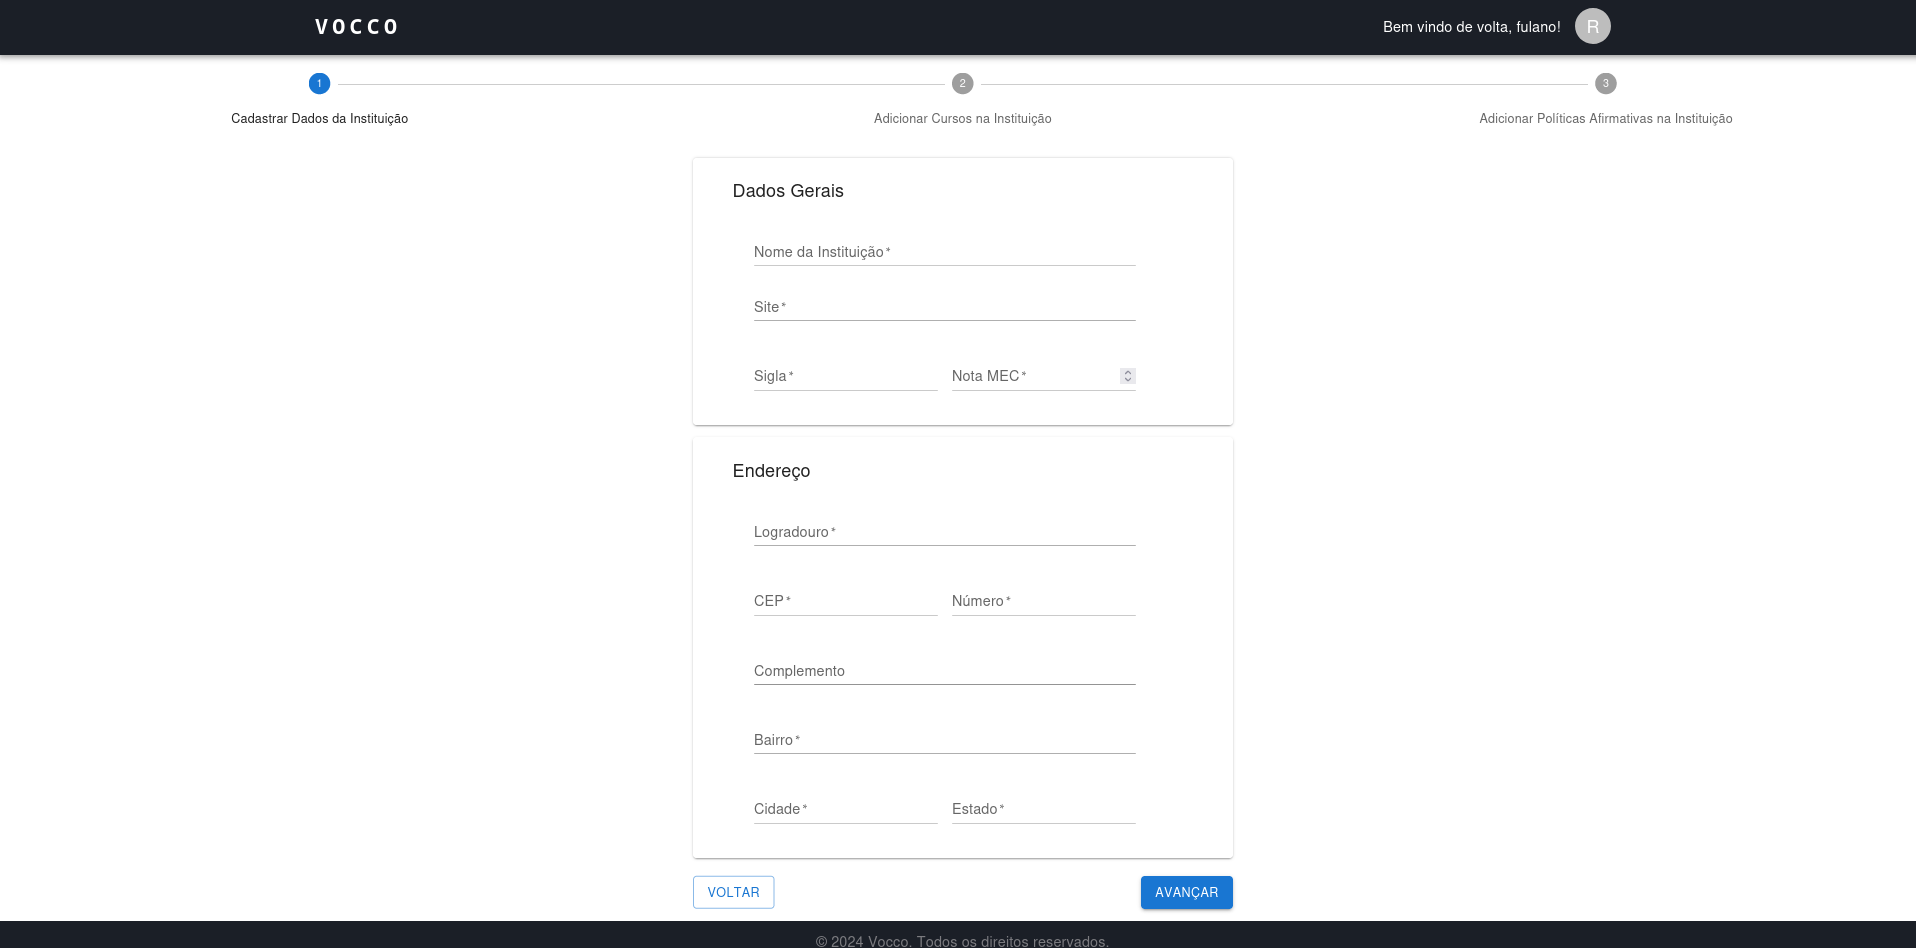
\includegraphics[width=1.0\linewidth]{images/dadosGerais.png}
    \caption{Cadastro de dados gerais da instituição}
    \label{fig:dados-gerais}
\end{figure}

\section{Tela de gerenciamento de instituições}
\begin{figure}[H]
    \centering
    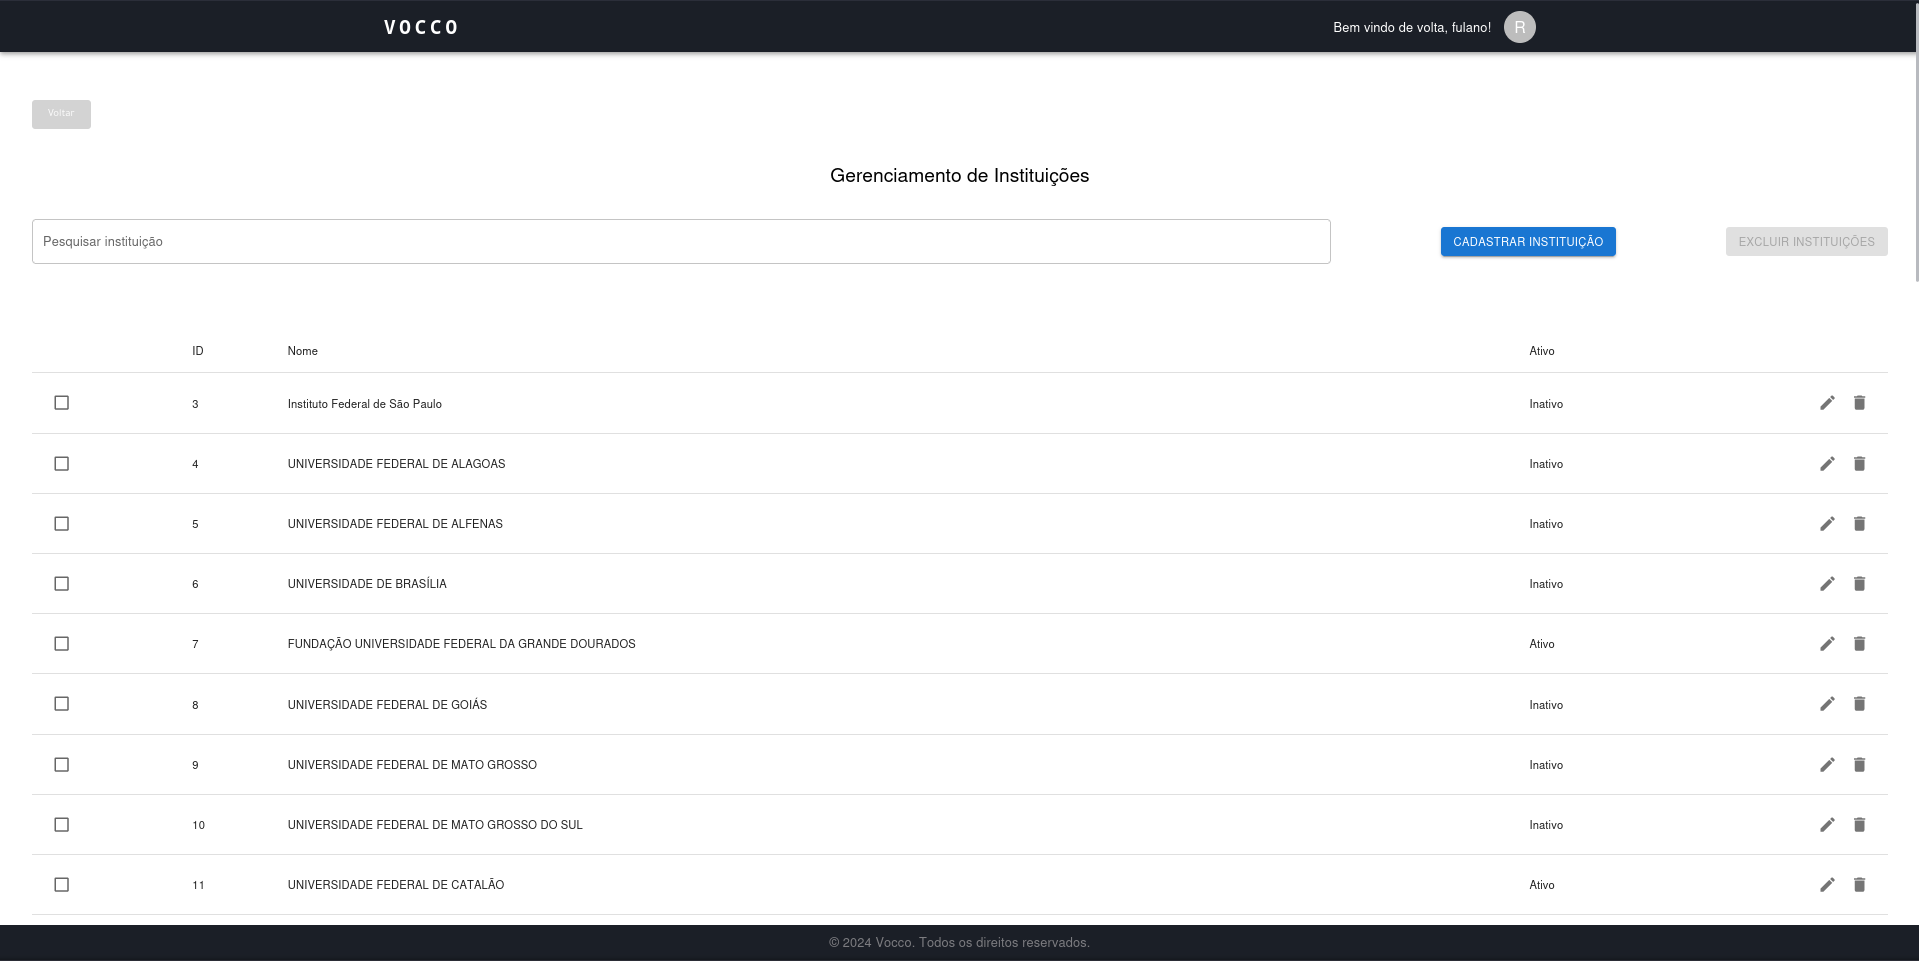
\includegraphics[width=1.0\linewidth]{images/gerenciamento.png}
    \caption{Gerenciamento de instituições}
    \label{fig:gerenciamento}
\end{figure}

\section{Tela de detalhamento de uma instituição}
\begin{figure}[H]
    \centering
    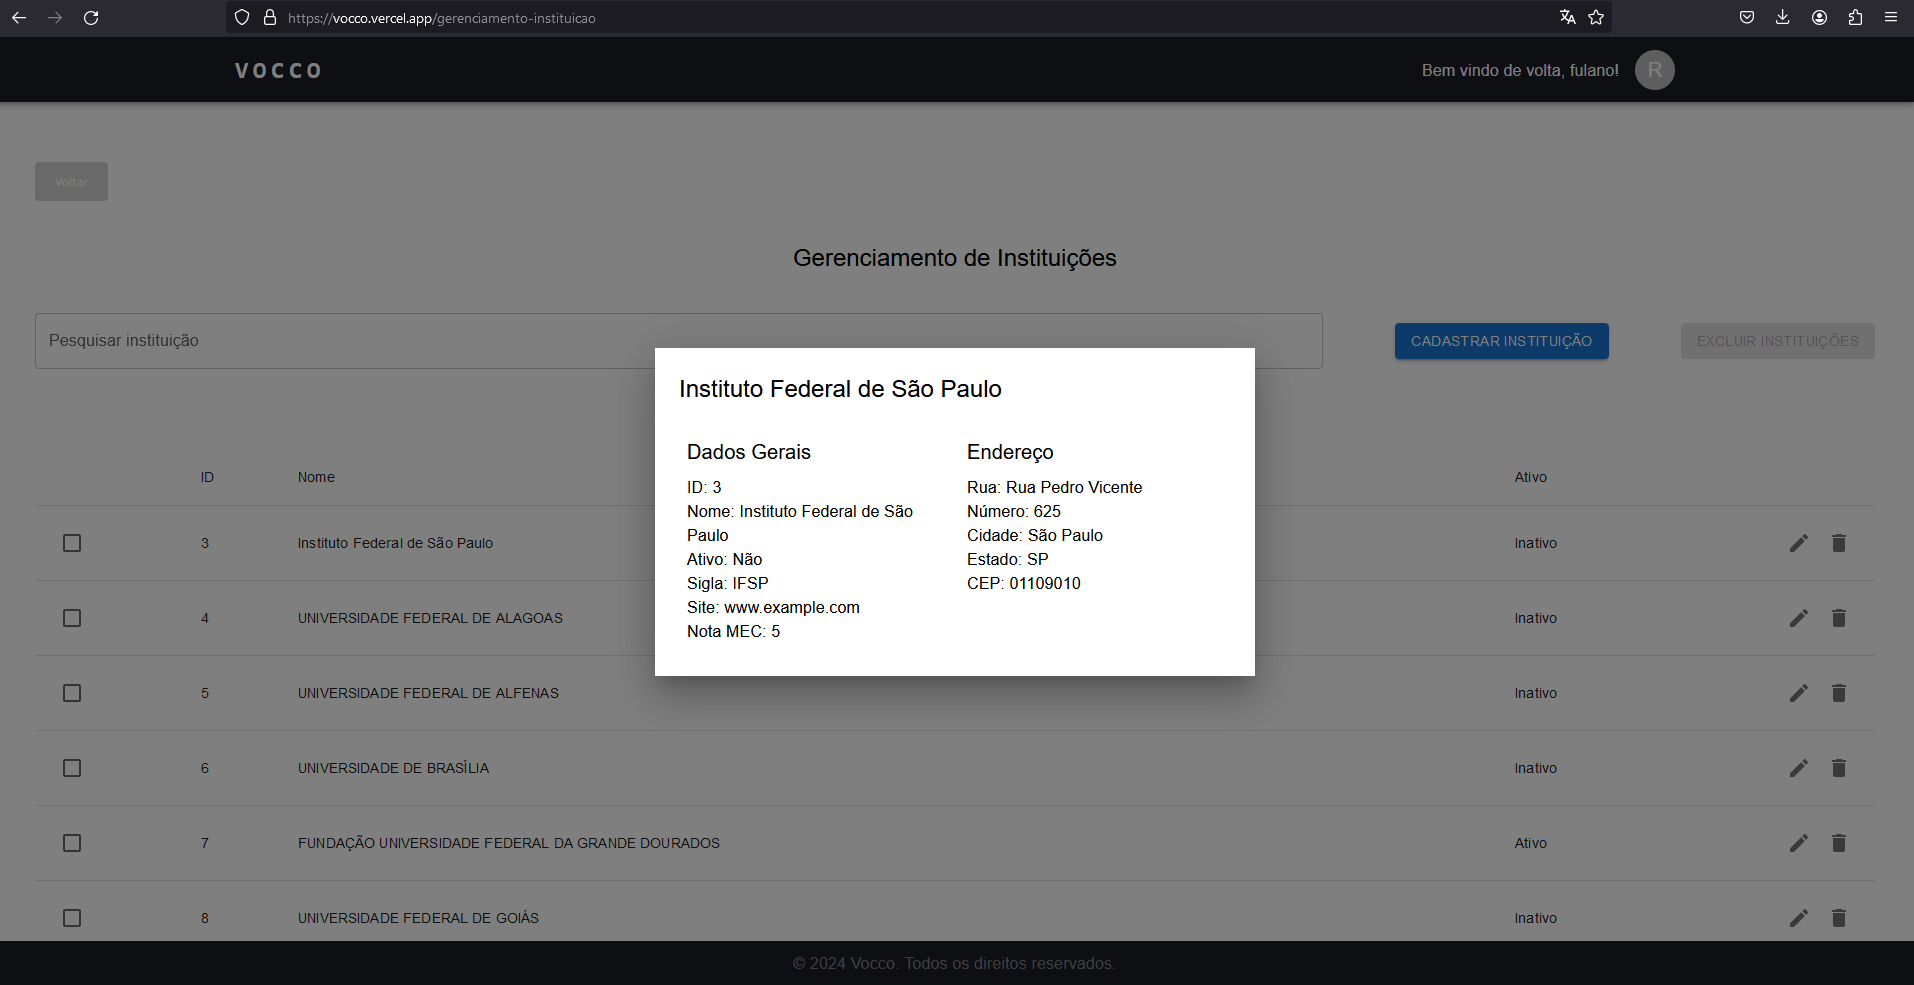
\includegraphics[width=1.0\linewidth]{images/informacoes.png}
    \caption{Cadastro de dados gerais da instituição}
    \label{fig:detalhamento}
\end{figure}

\section{Tela de edição de uma instituição}
\begin{figure}[H]
    \centering
    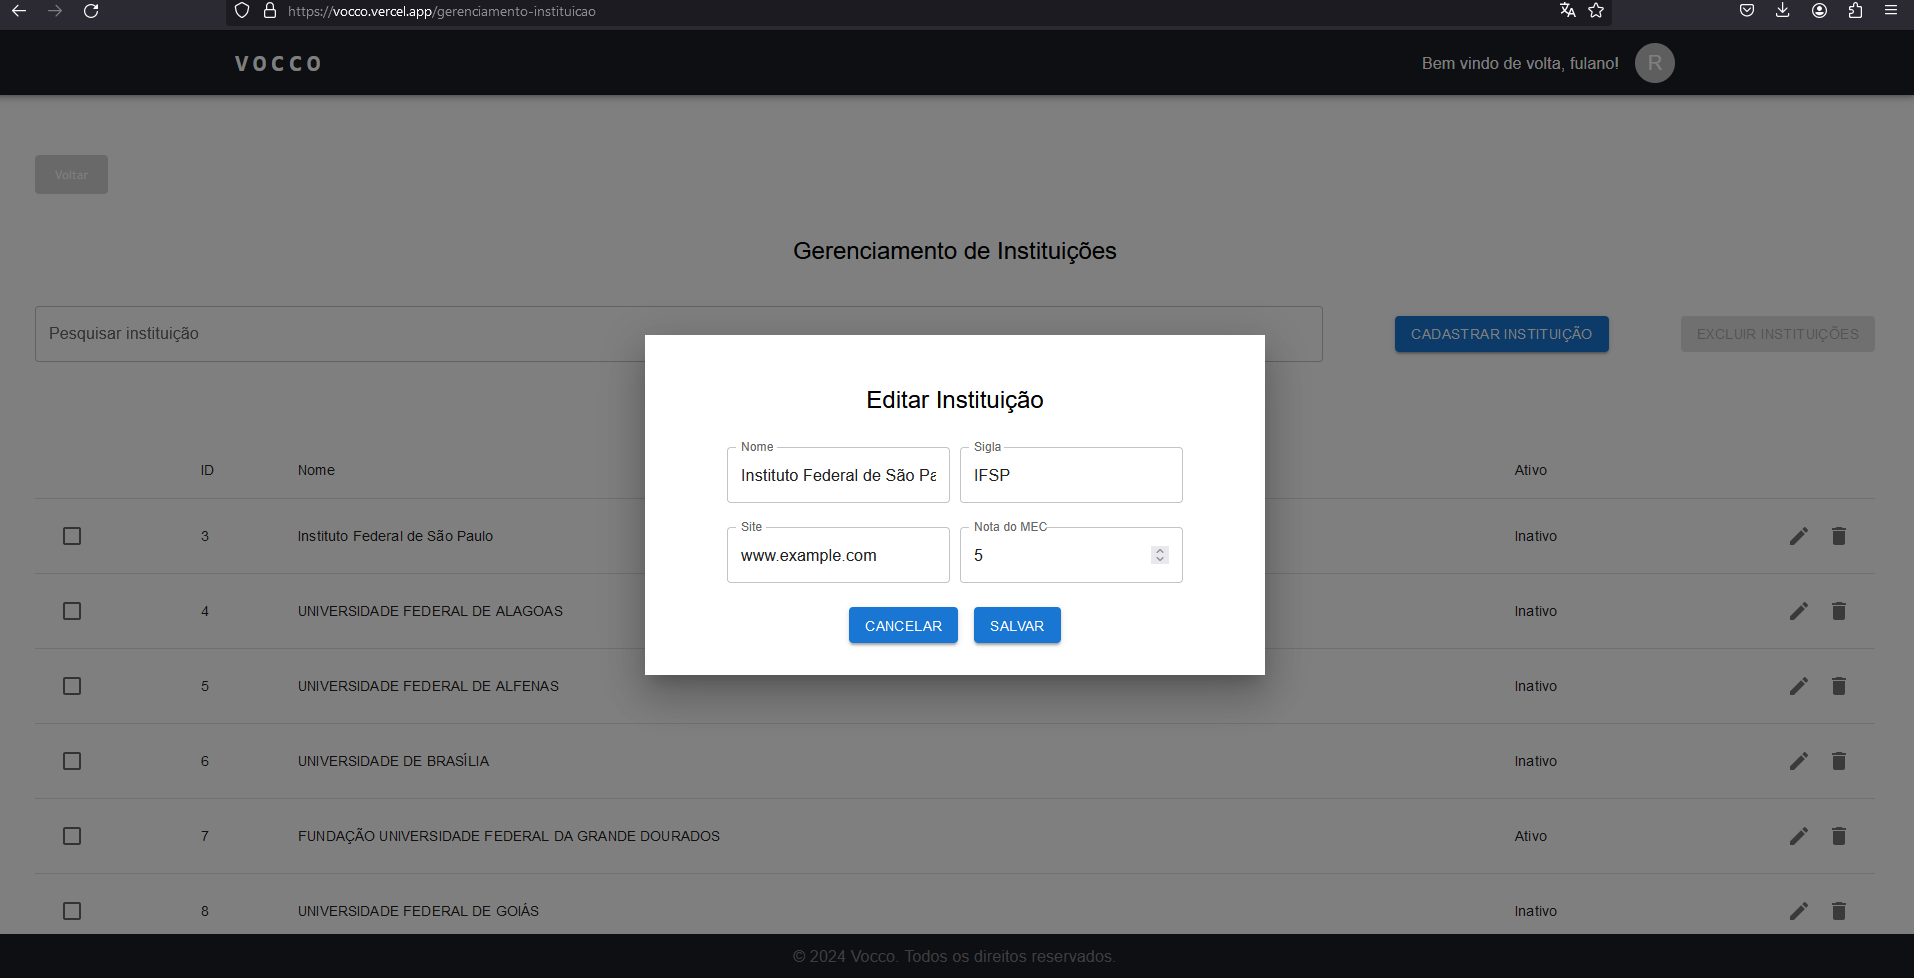
\includegraphics[width=1.0\linewidth]{images/editar.png}
    \caption{Cadastro de dados gerais da instituição}
    \label{fig:editar}
\end{figure}

\section{Tela de exclusão de uma instituição}
\begin{figure}[H]
    \centering
    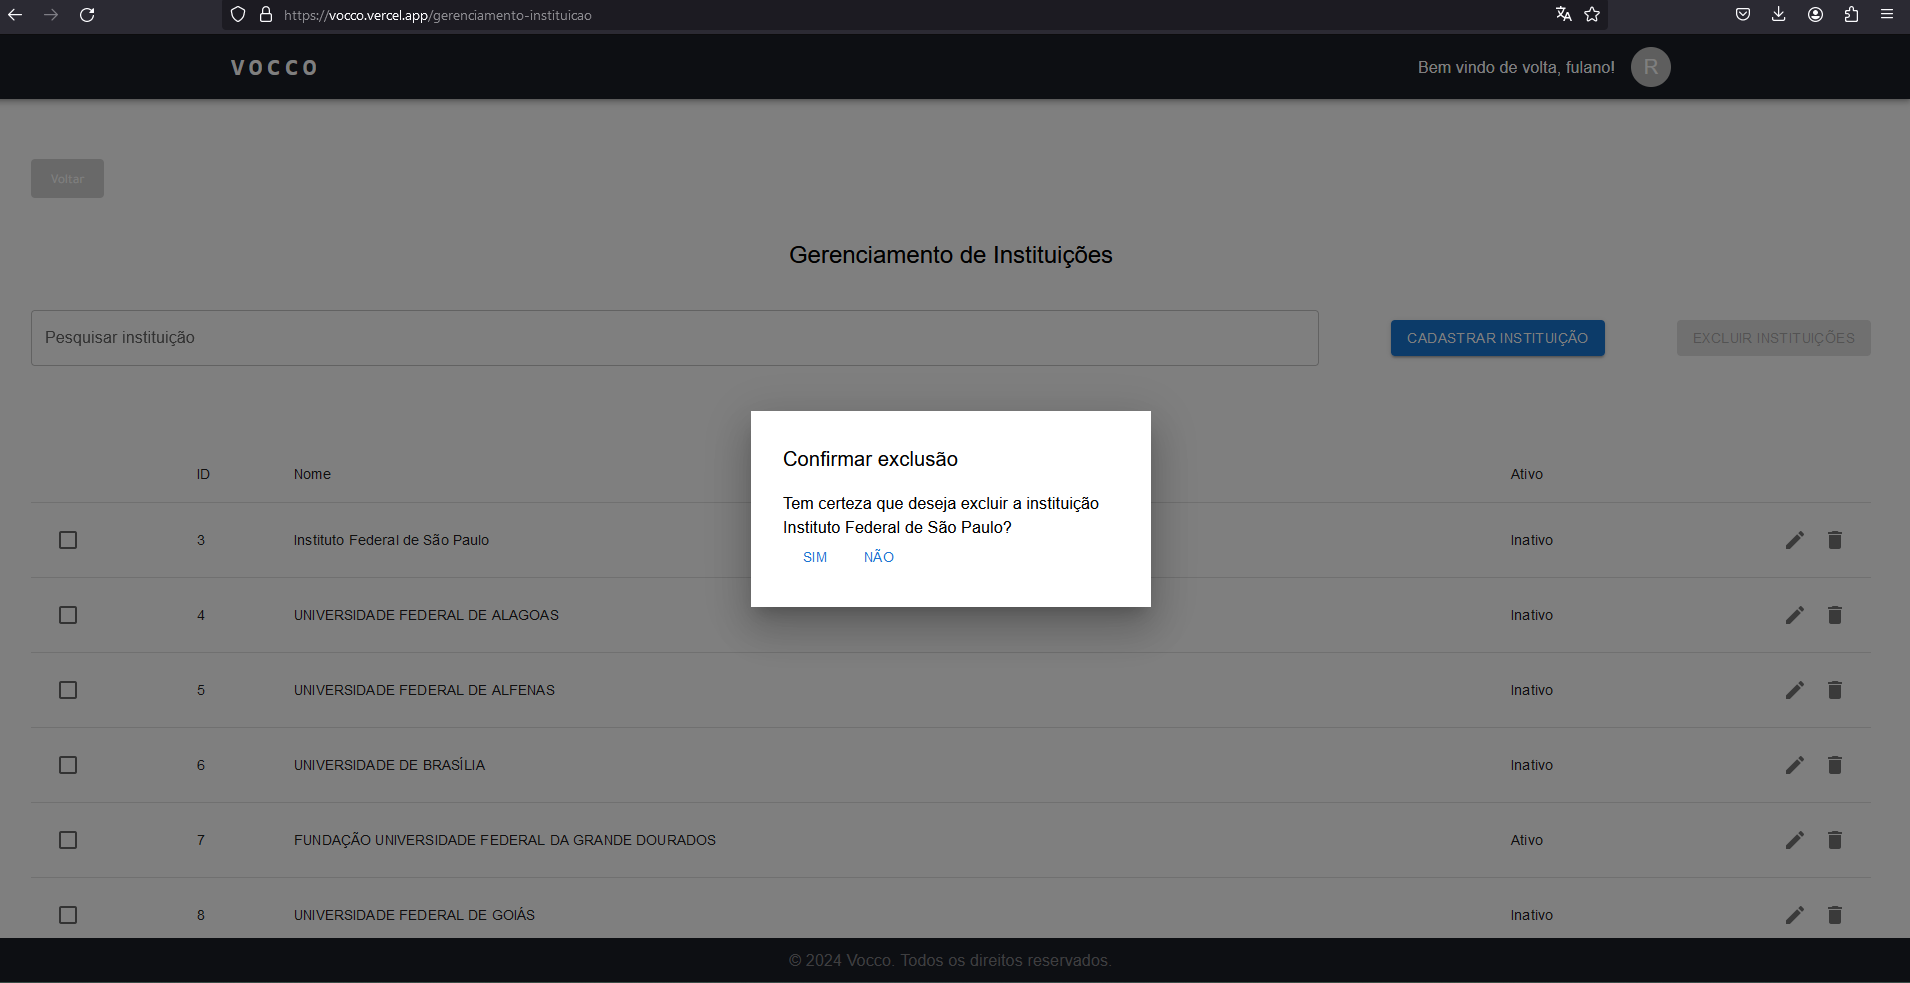
\includegraphics[width=1.0\linewidth]{images/exclusao.png}
    \caption{Cadastro de dados gerais da instituição}
    \label{fig:exclusao}
\end{figure}

\section{Tela de associação de instituições com cursos}
\begin{figure}[H]
    \centering
    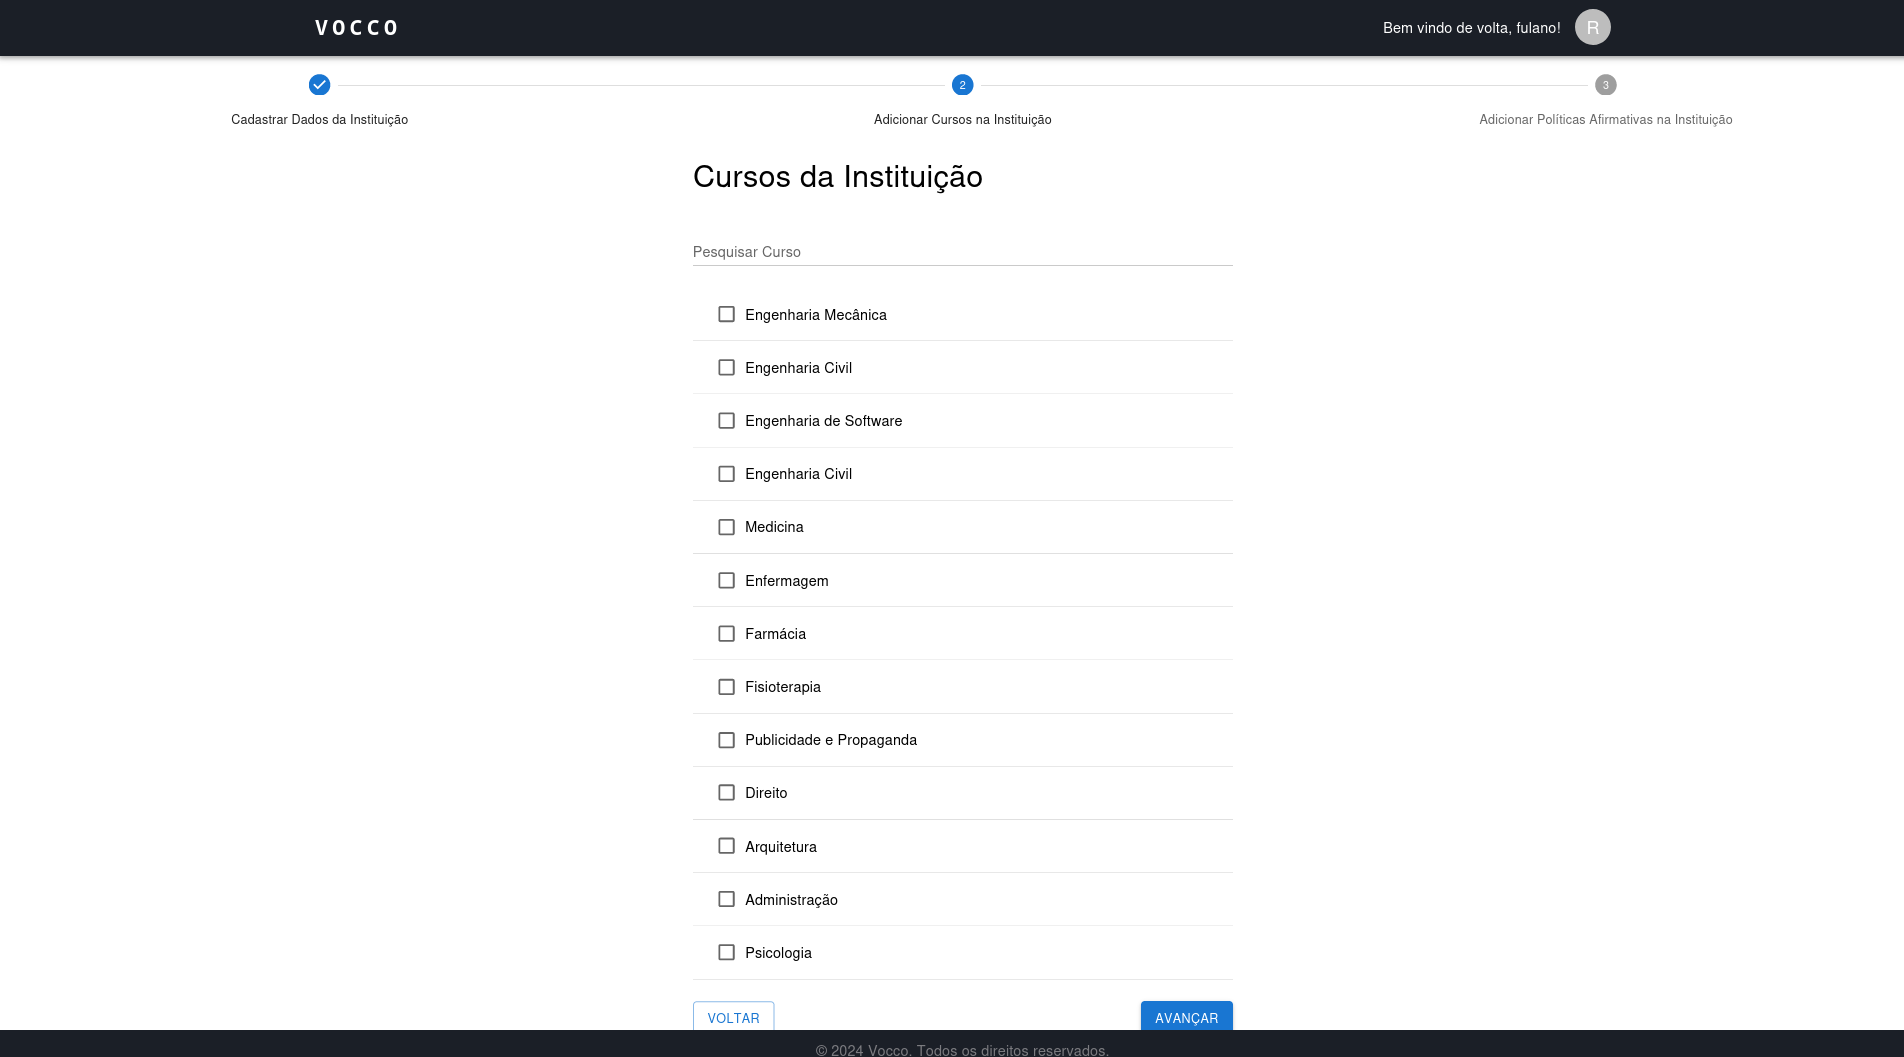
\includegraphics[width=1.0\linewidth]{images/cursos.png}
    \caption{Inserção dos cursos na instituição}
    \label{fig:cursos}
\end{figure}

\section{Tela de associação de instituições com políticas}
\begin{figure}[H]
    \centering
    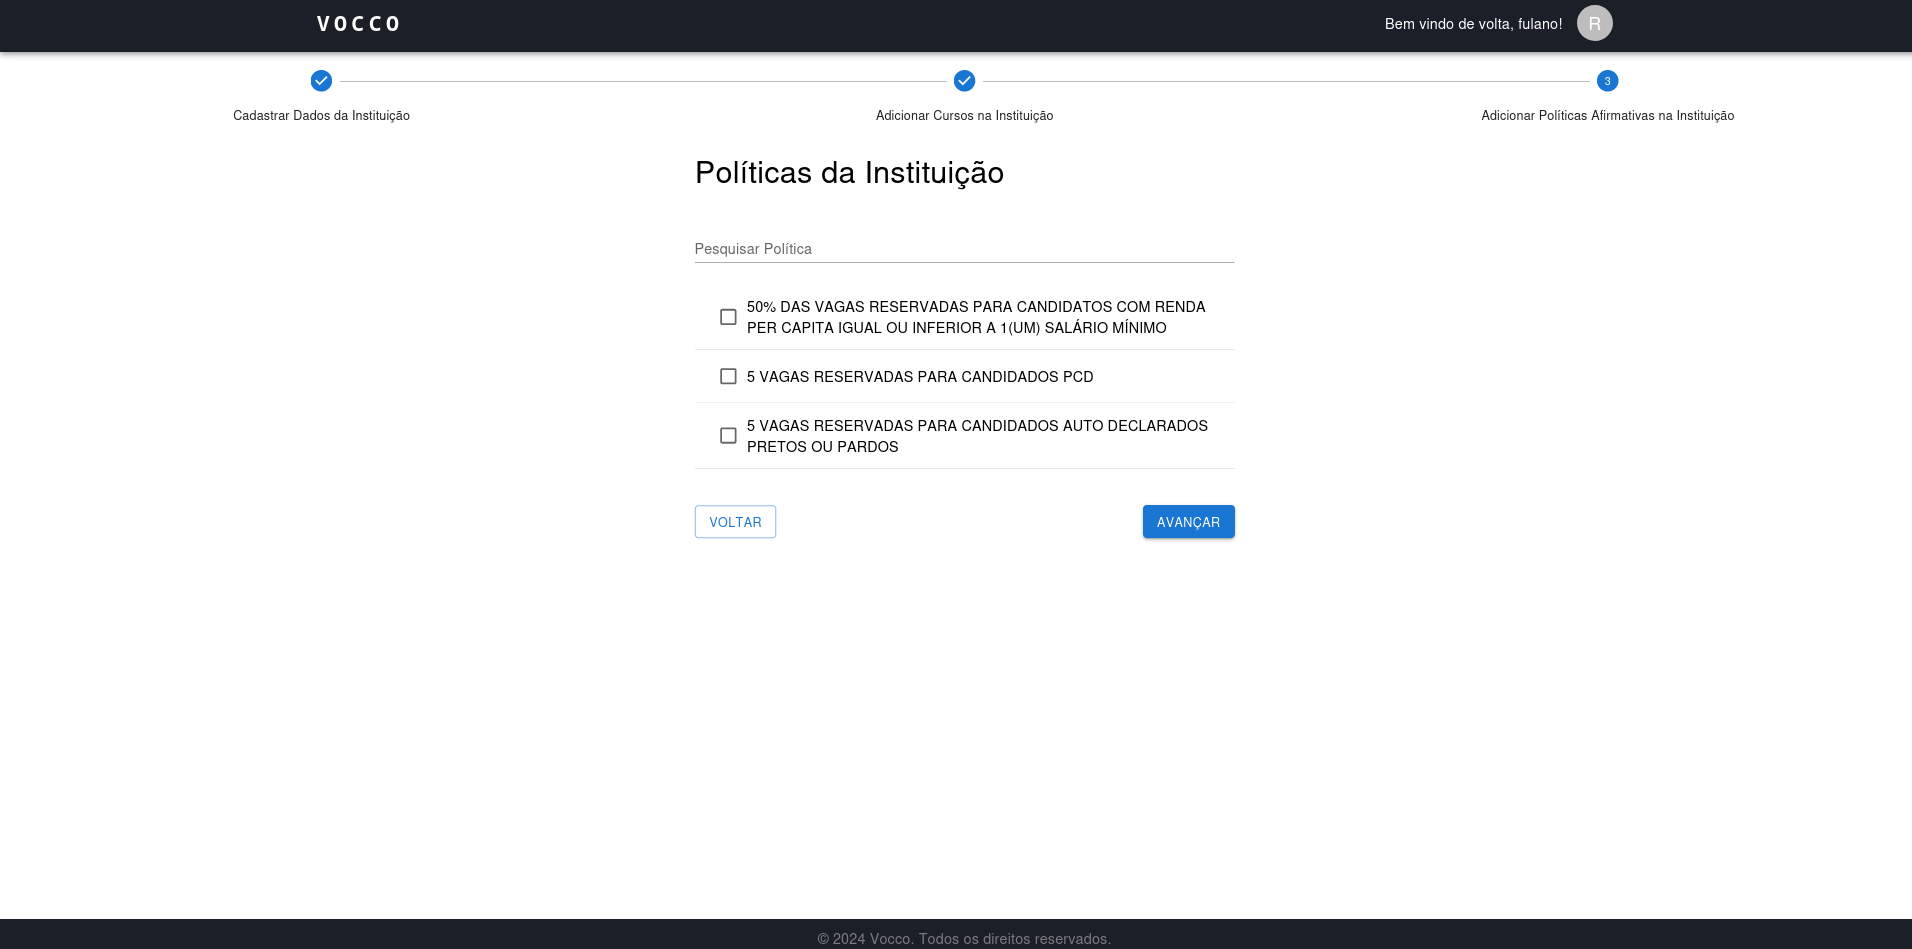
\includegraphics[width=1.0\linewidth]{images/politicas.png}
    \caption{Inserção das políticas na instituição}
    \label{fig:politicas}
\end{figure}

\chapter{Cronograma}
\label{apendice_i}
Para a organização e planejamento do desenvolvimento do projeto, dividimos as atribuições entre os integrantes do grupo. Dessa forma, conseguimos definir as datas de entrega e segui-las com mais facilidade. Com isso, o cronograma manteve um fluxo mais dinâmico e organizado, atendendo aos prazos estabelecidos para a entrega de cada fase do projeto.
\subsection*{Back-End}
Atividades e prazos definidos para o \textit{back-end} no decorrer do segundo semestre de 2024.

\begin{figure}[ht]
        \centering
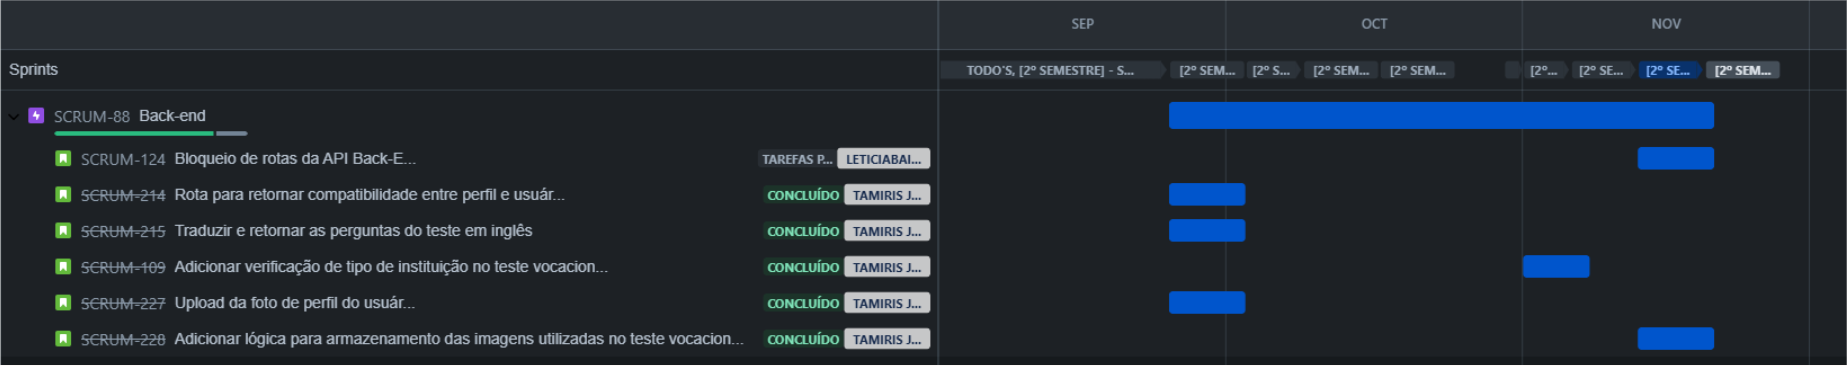
\includegraphics[width=1.0\textwidth]{images/back-end-cronograma.png}
        \caption{Cronograma definido para o \textit{back-end} no segundo semestre de 2024}
        \label{fig:backendcronograma}
    \end{figure}
As atividades do \textit{back-end} foram em sua maior parte concluídas no primeiro semestre de 2024, sendo que no segundo semestre foram feitos somentes ajustes necessários.    
\newpage
    
\subsection*{Base de Dados}
Atividades e prazos definidos para a realização de cadastros na base de dados no decorrer do segundo semestre de 2024. 

\begin{figure}[ht]
        \centering
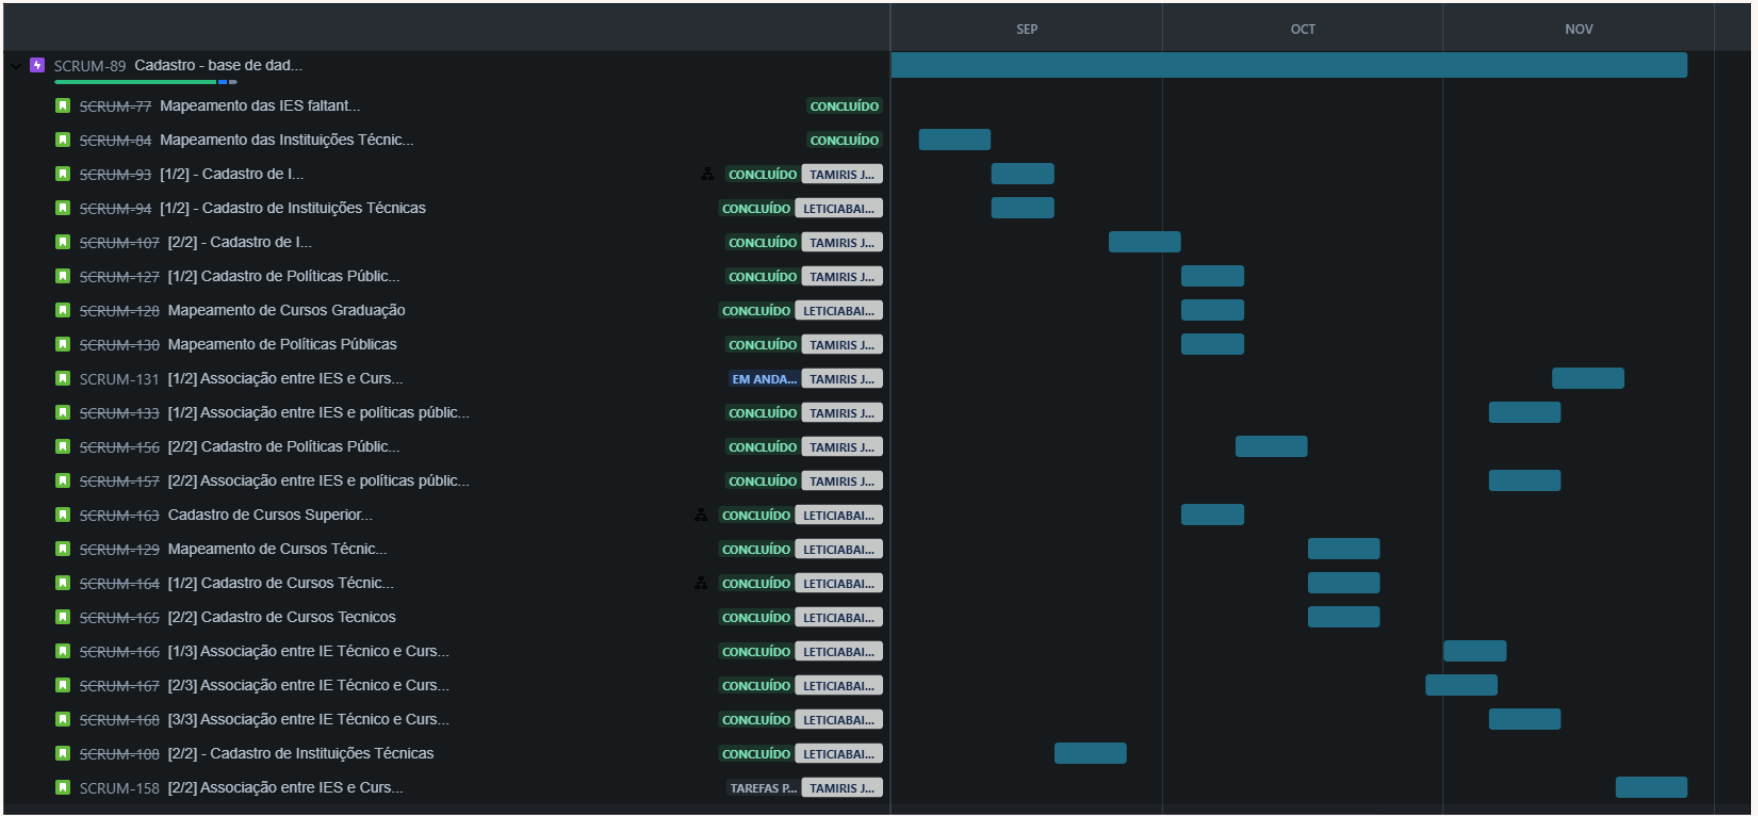
\includegraphics[width=1.0\textwidth]{images/base-dados-cronograma.png}
        \caption{Cronograma definido para os cadastros na base de dados no segundo semestre de 2024}
        \label{fig:basedadoscronograma}
    \end{figure}
As integrantes do grupo responsáveis pelo \textit{back-end} ficaram responsáveis pelos cadastros na base de dados no segundo semestre.

\subsection*{Design Visual}
Atividades e prazos definidos para a finalização do design visual do projeto no decorrer do segundo semestre de 2024. 

\begin{figure}[ht]
        \centering
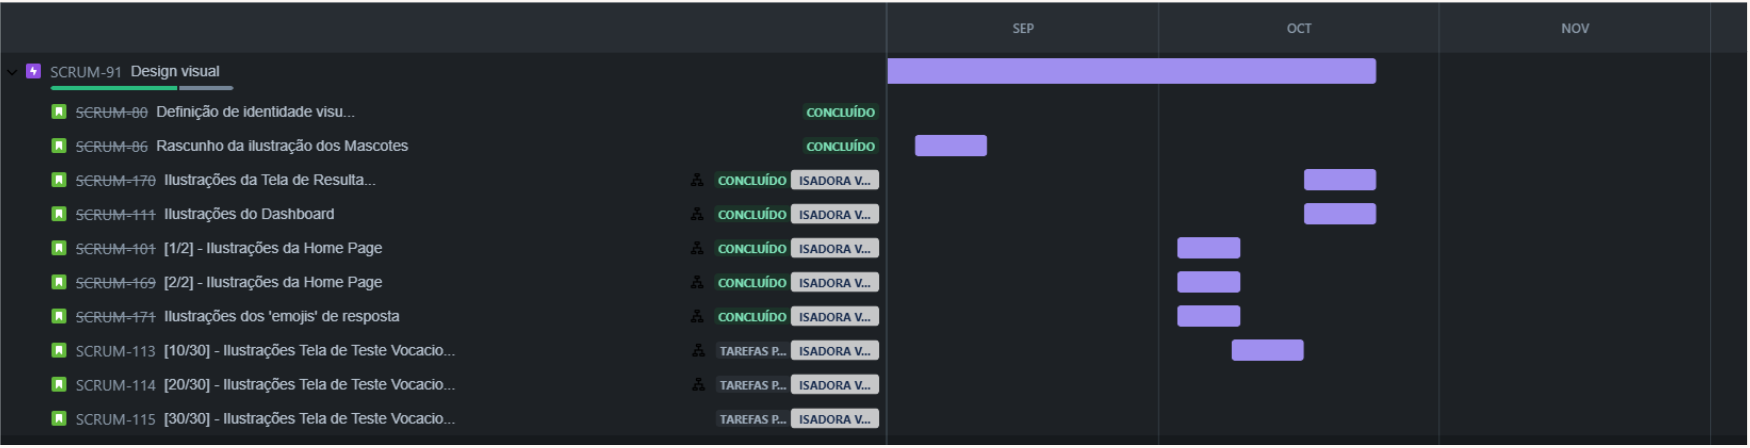
\includegraphics[width=1.0\textwidth]{images/design-visual-cronograma.png}
        \caption{Cronograma definido para o design visual no segundo semestre de 2024}
        \label{fig:designvisualcronograma}
    \end{figure}
\newpage

Com a refatoração da telas, se fez necessário novos designs visuais para o projeto.

\subsection*{Front-End}
Atividades e prazos definidos para o \textit{back-end} no decorrer do segundo semestre de 2024.

\begin{figure}[ht]
        \centering
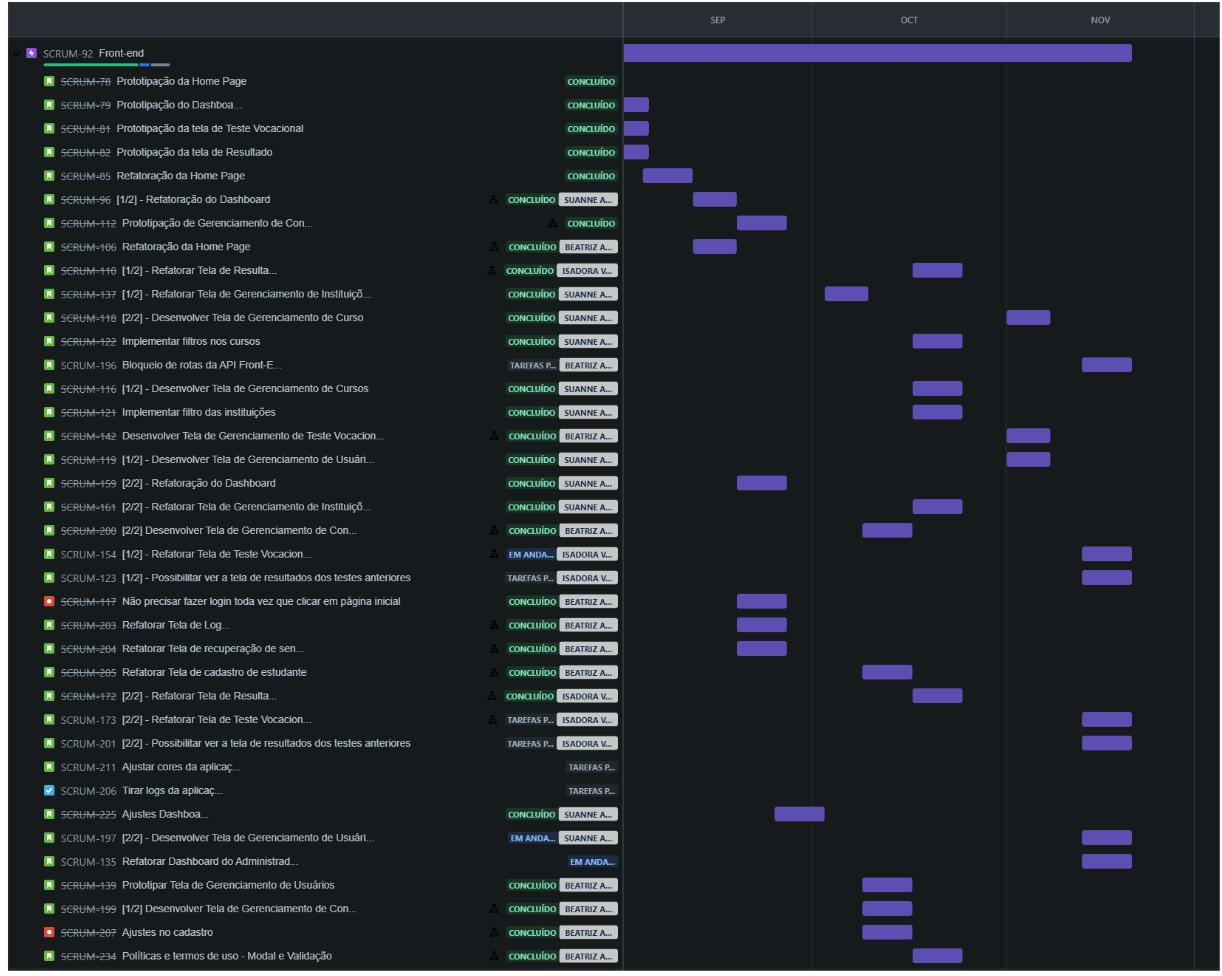
\includegraphics[width=1.0\textwidth]{images/front-end-cronograma.png}
        \caption{Cronograma definido para o \textit{front-end} no segundo semestre de 2024}
        \label{fig:frontendcronograma}
    \end{figure}
\newpage

Com a refatoração da telas, o front-end ficou com mais tarefas que o \textit{back-end}.

\subsection*{Revisões e Documentação}
Atividades e prazos definidos para finalizar as tarefa de revisão e documentação no decorrer do segundo semestre de 2024.

\begin{figure}[ht]
        \centering
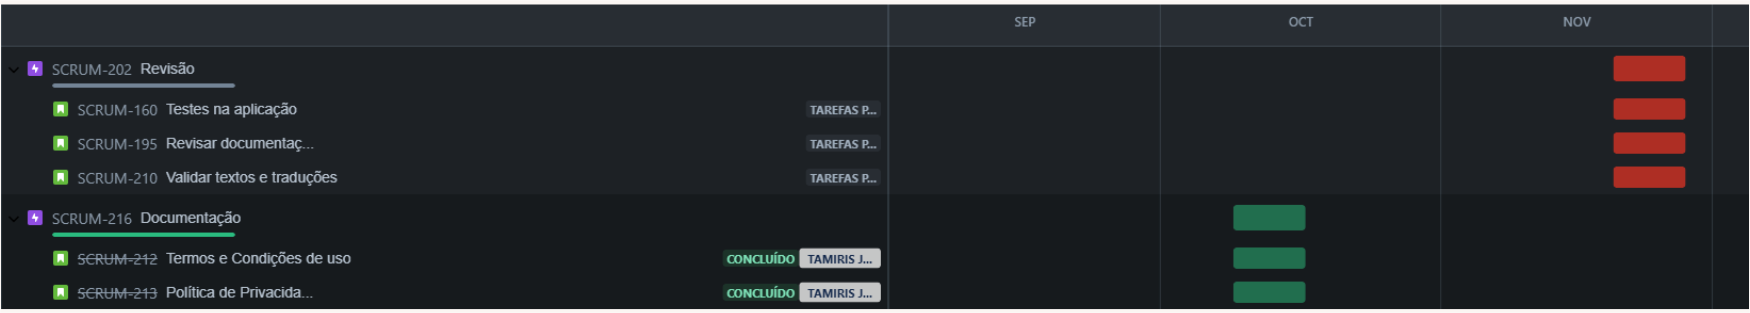
\includegraphics[width=1.0\textwidth]{images/revisao-cronograma.png}
        \caption{Cronograma definido para a revisão e documentação no segundo semestre de 2024}
        \label{fig:revisaocronograma}
    \end{figure}

O desenvolvimento do projeto e a documentação são extensos e demandam reuniões constantes para verificar o progresso e ajustar o que ainda precisa ser feito. Dessa forma, as reuniões de planejamento e verificação continuam acontecendo para garantir que a entrega final do projeto seja realizada dentro do prazo.

\chapter{TESTE DE USABILIDADE - RESULTADOS}
\label{apendice_l}

\begin{figure}[H]
    \centering
    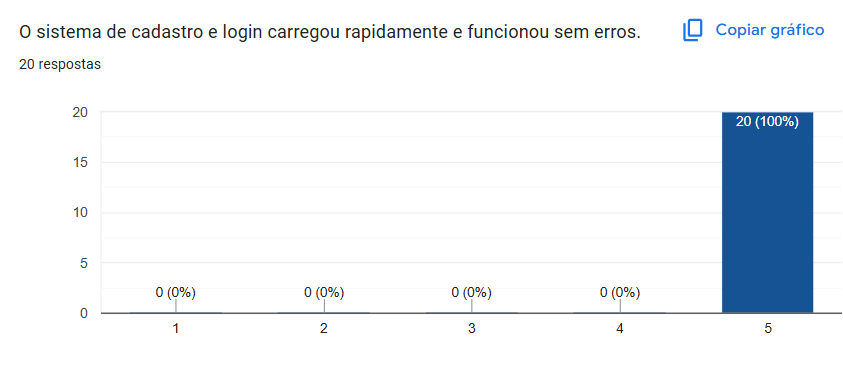
\includegraphics[width=1.0\linewidth]{images/cadastro.png}
    \caption{Processo de cadastro e login}
    \label{fig:cadastro}
\end{figure}

\begin{figure}[H]
    \centering
    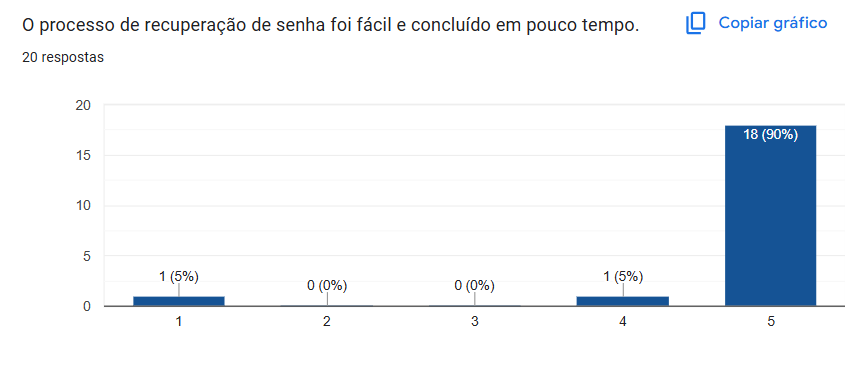
\includegraphics[width=1.0\linewidth]{images/recuperacao.png}
    \caption{Processo de recuperação de senha}
    \label{fig:senha}
\end{figure}

\begin{figure}[H]
    \centering
    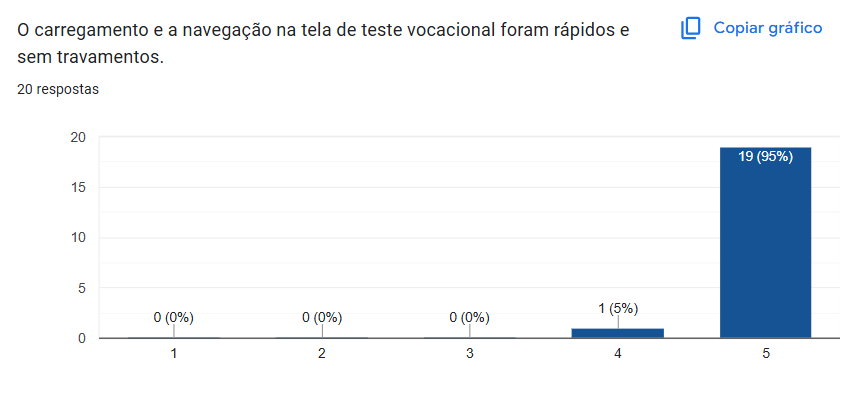
\includegraphics[width=1.0\linewidth]{images/teste.png}
    \caption{Resposta do teste vocacional}
    \label{fig:teste}
\end{figure}

\begin{figure}[H]
    \centering
    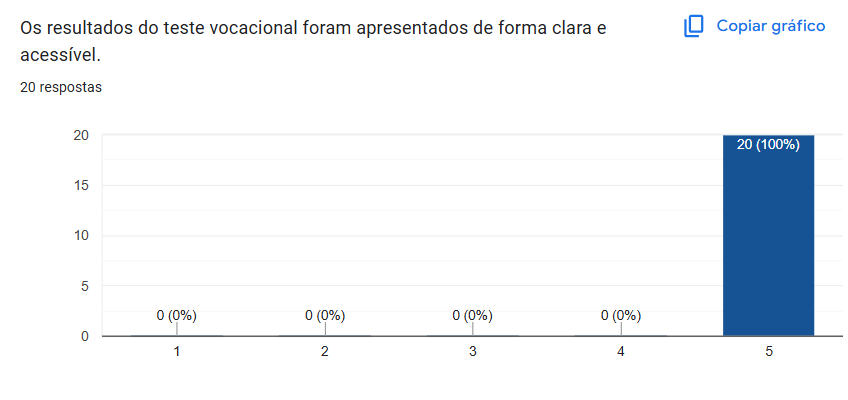
\includegraphics[width=1.0\linewidth]{images/resultado.png}
    \caption{Resultado do teste vocacional}
    \label{fig:resultado}
\end{figure}

\begin{figure}[H]
    \centering
    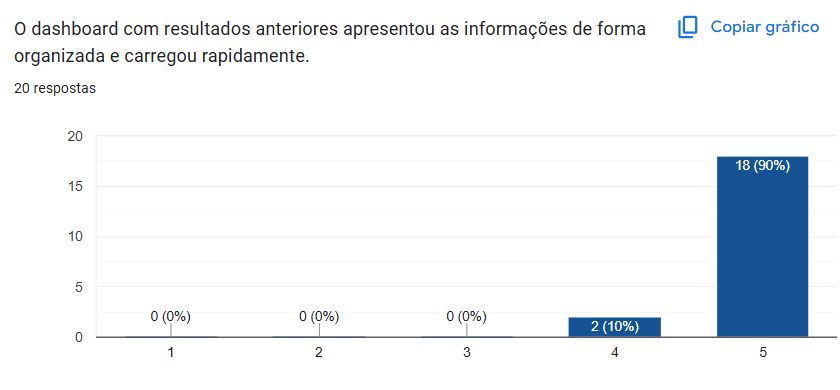
\includegraphics[width=1.0\linewidth]{images/resultadoAnterior.png}
    \caption{Dashboard}
    \label{fig:resultadoAnterior}
\end{figure}

\begin{figure}[H]
    \centering
    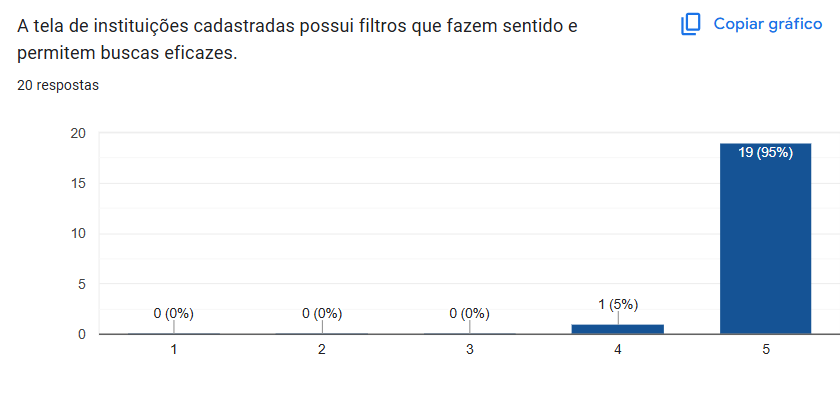
\includegraphics[width=1.0\linewidth]{images/instituicoes.png}
    \caption{Listagem de instituições}
    \label{fig:instituicoes}
\end{figure}

\begin{figure}[H]
    \centering
    \includegraphics[width=1.0\linewidth]{images/cursosListagem.png}
    \caption{Listagem de cursos}
    \label{fig:cursos}
\end{figure}

\begin{figure}[H]
    \centering
    \includegraphics[width=1.0\linewidth]{images/conta.png}
    \caption{Gerenciamento de conta}
    \label{fig:conta}
\end{figure}


\begin{figure}[H]
    \centering
    \includegraphics[width=1.0\linewidth]{images/fotoPerfil.png}
    \caption{Adição da foto de perfil}
    \label{fig:fotoPerfil}
\end{figure}

\begin{figure}[H]
    \centering
    \includegraphics[width=1.0\linewidth]{images/relevanciaCursos.png}
    \caption{Relevância da tela de listagem de cursos}
    \label{fig:relevanciaCursos}
\end{figure}

\begin{figure}[H]
    \centering
    \includegraphics[width=1.0\linewidth]{images/relevanciaInstituicao.png}
    \caption{Relevância da tela de listagem de instituições}
    \label{fig:relevanciaInstituicoes}
\end{figure}

\begin{figure}[H]
    \centering
    \includegraphics[width=1.0\linewidth]{images/relevanciaTeste.png}
    \caption{Relevância do teste vocacional}
    \label{fig:relevanciaTeste}
\end{figure}


\begin{figure}[H]
    \centering
    \includegraphics[width=0.85\linewidth]{images/sugestões1.png}
    \caption{Sugestões de melhoria}
    \label{fig:sugestoes}
\end{figure}


\begin{figure}[H]
    \centering
    \includegraphics[width=0.85\linewidth]{images/sugestões2.png}
    \caption{Sugestões de melhoria}
    \label{fig:sugestoes}
\end{figure}


\begin{figure}[H]
    \centering
    \includegraphics[width=0.85\linewidth]{images/sugestões3.png}
    \caption{Sugestões de melhoria}
    \label{fig:sugestoes}
\end{figure}

\chapter{Atas de Reuniões}
\label{apendice_j}

\section*{Reunião 10/03}

\subsection*{Participantes}
Beatriz Andrade, Isadora Câmara, Letícia Baião, Suanne Almeida, Tamiris Jesus.

\subsection*{Pauta}
\begin{itemize}
    \item Estudo de viabilidade do projeto, considerando o fluxo de atividades necessárias para a sua realização.
    \item Desenvolvimento e organização do documento de introdução.
    \item Divisão dos temas a serem abordados na apresentação da próxima semana.
\end{itemize}

\subsection*{Observações}
Primeira reunião realizada, marcando o início oficial do projeto. 
Decisão de cada membro gravar sua parte da apresentação para posterior edição em um vídeo a ser publicado no canal da equipe no YouTube. 

\subsection*{Ações Necessárias}
\begin{itemize}
    \item Definição da proposta da plataforma e seus objetivos.
    \item Análise das propostas para o desenvolvimento do cálculo de compatibilidade a ser utilizado no teste vocacional.
    \item Estudo de ideias para potenciais fontes de financiamento e oportunidades de parcerias.
    \item Transferência do documento de introdução para o Overleaf.
    \item Início da elaboração dos slides para a apresentação.
\end{itemize}

\subsection*{Pauta da Próxima Semana}
Para a próxima semana, ficou definido que iremos unir as partes gravadas por cada integrante para o vídeo.

\section*{Reunião 13/03}

\subsection*{Participantes}
Beatriz Andrade, Isadora Câmara, Letícia Baião, Tamiris Jesus, Suanne Almeida.

\subsection*{Pauta}
\begin{itemize}
    \item Acompanhamento da última reunião: Os vídeos de cada integrante foram agrupados em um único vídeo, o qual já foi publicado no canal do YouTube da equipe, conforme o proposto na reunião anterior. 
    \item Novos assuntos:
    \begin{itemize}
        \item Discussão sobre o algoritmo responsável pelo cálculo de compatibilidade a ser utilizado no teste vocacional.
        \item Definição de cargos para cada membro da equipe.
        \item Análise de estratégias para o controle de versão.
        \item Análise de estratégias para a documentação.
    \end{itemize}
\end{itemize}

\subsection*{Observações}
Não foi realizada uma reunião para consolidar as partes dos vídeos gravados por cada integrante em um único vídeo.
Cada membro da equipe assumiu a responsabilidade de realizar pesquisas referentes à proposta do projeto e analisar o funcionamento dos testes vocacionais em plataformas concorrentes.

\subsection*{Ações Necessárias}
\begin{itemize}
    \item Avaliação de perspectivas sobre o algoritmo a ser usado no cálculo de compatibilidade, juntamente com as suposições relacionadas às funcionalidades e ao fluxo.
    \item Análise das habilidades/afinidades individuais de cada integrante para determinar a área em que melhor se encaixa no projeto.
    \item Avaliação e decisão sobre qual método de ramificação utilizar para o controle de versão.
    \item Definição das ferramentas de documentação a serem utilizadas.
\end{itemize}

\subsection*{Pauta da Próxima Semana}
\begin{itemize}
    \item Apresentar os resultados e sugestões de aprimoramento dos testes vocacionais a serem analisados.
    \item \textit{Brainstorming} de funcionalidades para o sistema.
    \item Elaborar uma proposta de projeto para concorrer ao Prêmio Luz na Educação.
\end{itemize}

\section*{Reunião 20/03}

\subsection*{Participantes}
Beatriz Andrade, Isadora Câmara, Letícia Baião, Tamiris Jesus, Suanne Almeida.

\subsection*{Pauta}
\begin{itemize}
    \item Acompanhamento da última reunião: Cada membro da equipe cumpriu sua responsabilidade ao realizar pesquisas sobre a proposta do projeto e analisar o funcionamento dos testes vocacionais em plataformas concorrentes.
    \item Novos assuntos:
    \begin{itemize}
        \item Discussão sobre como funciona o \ac{svn} e como subiremos nossos arquivos, incluindo o compartilhamento do link do YouTube, a apresentação de slides e o documento de introdução.
        \item Análise dos testes vocacionais realizados em plataformas concorrentes.
    \end{itemize}
\end{itemize}

\subsection*{Observações}
O brainstorming de funcionalidades para o sistema e a elaboração de uma proposta de projeto para concorrer ao Prêmio Luz na Educação não foram realizados.

\subsection*{Ações Necessárias}
\begin{itemize}
    \item Cada integrante compartilhou suas experiências com os testes vocacionais, discutindo o que mais gostaram, o que menos gostaram, as vantagens e as desvantagens.
    \item Análise do que de positivo podemos extrair dos testes vocacionais estudados para aplicar em nosso projeto.
    \item Pré-seleção dos requisitos para os testes vocacionais.
\end{itemize}

\subsection*{Pauta da Próxima Semana}
\begin{itemize}
    \item Definição de requisitos, incluindo requisitos funcionais, não funcionais e regras de negócio.
    \item Brainstorming de funcionalidades para o sistema.
    \item Elaborar uma proposta de projeto para concorrer ao Prêmio Luz na Educação.
\end{itemize}

\section*{Reunião 27/03}

\subsection*{Participantes}
Beatriz Andrade, Isadora Câmara, Tamiris Jesus, Suanne Almeida.

\subsection*{Pauta}
\begin{itemize}
    \item Novos assuntos:
    \begin{itemize}
        \item Discussão sobre as funcionalidades do sistema e as entidades que serão implementadas.
        \item Discussão sobre as vantagens das tecnologias que serão utilizadas no frontend.
        \item Início da definição de requisitos, abrangendo requisitos funcionais, não funcionais e regras de negócio.
    \end{itemize}
\end{itemize}

\subsection*{Observações}
A definição dos requisitos do sistema não foi concluída e a elaboração de uma proposta de projeto para concorrer ao Prêmio Luz na Educação não foi realizada.
Foi sugerido que assistíssemos às aulas recomendadas por uma integrante do grupo sobre o uso do TypeScript em uma aplicação.

\subsection*{Ações Necessárias}
\begin{itemize}
    \item Discutimos as funcionalidades que nosso sistema terá, avaliando quais são essenciais para a fase atual e quais pretendemos implementar posteriormente.
    \item No contexto das funcionalidades, analisamos quais entidades seriam necessárias em nosso sistema.
    \item Discutimos as vantagens do React e do TypeScript, bem como as otimizações que essas tecnologias trariam para o projeto.
    \item Elaboração de um documento que contém os requisitos, abrangendo tanto os requisitos funcionais quanto os não funcionais, além das regras de negócio.
\end{itemize}

\subsection*{Pauta da Próxima Semana}
\begin{itemize}
    \item Continuação da definição de requisitos, incluindo requisitos funcionais, não funcionais e regras de negócio.
    \item Início do esboço do desenho da arquitetura da aplicação.
    \item Elaborar uma proposta de projeto para concorrer ao Prêmio Luz na Educação.
\end{itemize}

\section*{Reunião 28/03}

\subsection*{Participantes}
Beatriz Andrade, Isadora Câmara, Letícia Baião, Tamiris Jesus, Suanne Almeida.

\subsection*{Pauta}
\begin{itemize}
    \item Novos assuntos:
    \begin{itemize}
        \item Atualização para todos os membros sobre as entidades do sistema e esclarecimento de dúvidas/inseguranças referentes à implantação do sistema na Amazon Web Service.
        \item Definição de todos os elementos que precisam ser incluídos no desenho da aplicação.
        \item Elaboração da proposta e inscrição para o Prêmio Luz na Educação.
    \end{itemize}
\end{itemize}

\subsection*{Observações}
Não foi proposta uma alternativa definitiva para substituir a implantação do sistema na \textbf{Amazon Web Service}.

\subsection*{Ações Necessárias}
\begin{itemize}
    \item Discutimos os prós e contras de implantar a plataforma na \textbf{Amazon Web Service}.
    \item Dividimos as partes que devem ser escritas para elaborar a documentação do desenho da aplicação entre as integrantes.
    \item Lemos o rascunho da proposta elaborado pela integrante Tamiris e realizamos os ajustes e melhorias necessários.
    \item Lemos a documentação do Prêmio Luz na Educação e seguimos todas as etapas necessárias para a inscrição.
\end{itemize}

\subsection*{Pauta da Próxima Semana}
\begin{itemize}
    \item Cada integrante será responsável por realizar a sua parte na documentação dos desenhos da aplicação.
    \item Ficou definido que as integrantes irão estudar e avaliar outras propostas para substituir a \textbf{Amazon Web Service} como plataforma de infraestrutura.
\end{itemize}

\section*{Reunião 03/04}

\subsection*{Participantes}
Beatriz Andrade, Isadora Câmara, Letícia Baião, Tamiris Jesus, Suanne Almeida.

\subsection*{Pauta}
\begin{itemize}
    \item Novos assuntos:
    \begin{itemize}
        \item Escolha de publicar toda a documentação no GitHub.
        \item Divisão das responsabilidades de criação dos slides entre as integrantes.
        \item Ajustes de configuração no \textbf{Overleaf}.
    \end{itemize}
\end{itemize}

\subsection*{Observações}
Após análises e estudos, as integrantes ficaram em dúvida entre duas plataformas para a implantação do sistema: \textbf{Heroku} e \textbf{Railway}.

\subsection*{Ações Necessárias}
\begin{itemize}
    \item Discutimos a divisão das responsabilidades na criação dos slides entre as integrantes.
    \item Foi feita a confirmação que a configuração do \textbf{Overleaf} que devemos utilizar é aquela enviada pelo professor.
    \item Nós definimos e validamos todos os requisitos do projeto.
    \item Decidimos que, a partir de agora, vamos incluir os áudios dos vídeos de apresentação diretamente nos slides do Canva.
\end{itemize}

\subsection*{Pauta da Próxima Semana}
\begin{itemize}
    \item As integrantes assumiram o compromisso de cada uma realizar sua parte nos slides, incluindo a gravação dos áudios a serem incorporados no Canva.
    \item As integrantes realizarão um estudo comparativo entre as plataformas Heroku e Railway para decidir qual delas deve ser utilizada para a infraestrutura.
\end{itemize}

\section*{Reunião 10/04}

\subsection*{Participantes}
Beatriz Andrade, Isadora Câmara, Letícia Baião, Tamiris Jesus, Suanne Almeida.

\subsection*{Pauta}
\begin{itemize}
    \item Novos assuntos:
    \begin{itemize}
        \item Análise da Prova de Conceito.
    \end{itemize}
\end{itemize}

\subsection*{Observações}
Reunião apenas para discutir a Prova de Conceito que deverá ser entregue.

\subsection*{Ações Necessárias}
\begin{itemize}
    \item Realizamos uma reunião em que discutimos minuciosamente e dividimos todas as etapas necessárias para a conclusão bem-sucedida da Prova de Conceito.
\end{itemize}

\subsection*{Pauta da Próxima Semana}
\begin{itemize}
    \item Ficou decidido que as integrantes começarão a trabalhar na documentação e se reunirão posteriormente para planejar o desenvolvimento do sistema.
\end{itemize}

\section*{Reunião 24/04}

\subsection*{Participantes}
Beatriz Andrade, Isadora Câmara, Letícia Baião, Tamiris Jesus, Suanne Almeida.

\subsection*{Pauta}
\begin{itemize}
    \item Novos assuntos:
    \begin{itemize}
        \item Escolha do modelo de referência para o código de personalidade que servirá de base para o teste vocacional.
        \item Escolha da ferramenta de construção para o \textit{frontend}.
    \end{itemize}
\end{itemize}

\subsection*{Observações}
A reunião também serviu para alinhar todas as integrantes quanto aos estudos em andamento, tanto no desenvolvimento \textit{backend} quanto no \textit{frontend}.

\subsection*{Ações Necessárias}
\begin{itemize}
    \item Realizamos uma pesquisa para identificar modelos de referência existentes para testes vocacionais ou avaliações de personalidade.
    \item Optamos por utilizar o modelo de código de personalidade de John Holland.
    \item Debatemos sobre as ferramentas de construção para o \textit{frontend} e optamos por utilizar o Vite.
\end{itemize}

\subsection*{Pauta da Próxima Semana}
\begin{itemize}
    \item Ficou decidido que as integrantes irão se reunir para elaborar como devem prosseguir no fluxo do desenvolvimento das telas.
\end{itemize}

\section*{Reunião 28/04}

\subsection*{Participantes}
Beatriz Andrade, Isadora Câmara, Letícia Baião, Tamiris Jesus, Suanne Almeida.

\subsection*{Pauta}
\begin{itemize}
    \item Novos assuntos:
    \begin{itemize}
        \item Desenvolvimento do \textit{design} das telas que serão implementadas no fluxo do perfil do administrador.
    \end{itemize}
\end{itemize}

\subsection*{Observações}
Como esses eram protótipos de baixa fidelidade, os desenhos das telas foram feitos no Canva.

\subsection*{Ações Necessárias}
\begin{itemize}
    \item As integrantes que estavam responsáveis pelo \textit{backend} orientaram as colegas encarregadas do \textit{frontend} no desenvolvimento das telas.
    \item Optamos por utilizar o modelo de código de personalidade de John Holland.
    \item Analisamos completamente os requisitos específicos do perfil do administrador e os fluxos que as telas devem suportar.
    \item Criamos \textit{wireframes} detalhados das telas.
\end{itemize}

\subsection*{Pauta da Próxima Semana}
\begin{itemize}
    \item Ficou decidido que as integrantes se reunirão para alinhar o desenvolvimento das telas.
\end{itemize}

\section*{Reunião 01/05}

\subsection*{Participantes}
Beatriz Andrade, Isadora Câmara, Letícia Baião, Tamiris Jesus, Suanne Almeida.

\subsection*{Pauta}
\begin{itemize}
    \item Novos assuntos:
    \begin{itemize}
        \item Discussão sobre o desenvolvimento das telas conforme os \textit{wireframes}.
        \item Atualização do progresso individual de cada integrante no projeto.
    \end{itemize}
\end{itemize}

\subsection*{Observações}
As telas estão sendo desenvolvidas de acordo com os protótipos de baixa fidelidade criados anteriormente.
Cada integrante compartilhou seu progresso e contribuições até o momento.

\subsection*{Ações Necessárias}
\begin{itemize}
    \item Implementação das alterações nos \textit{wireframes} conforme discutido.
    \item Continuação do desenvolvimento das telas com base nos requisitos estabelecidos.
\end{itemize}

\section*{Reunião 08/05}

\subsection*{Participantes}
Beatriz Andrade, Isadora Câmara, Letícia Baião, Tamiris Jesus, Suanne Almeida.

\subsection*{Pauta}
\begin{itemize}
    \item Novos assuntos:
    \begin{itemize}
        \item Discussão sobre os \textit{feedbacks} recebidos durante a apresentação.
        \item Planejamento dos próximos passos para a próxima entrega.
    \end{itemize}
\end{itemize}

\subsection*{Observações}
Como esses eram protótipos de baixa fidelidade, os desenhos das telas foram feitos no Canva.

\subsection*{Ações Necessárias}
\begin{itemize}
    \item O projeto foi apresentado e bem recebido pelo professor orientador.
    \item Foram discutidas melhorias sugeridas pelos \textit{feedbacks} recebidos.
\end{itemize}

\subsection*{Pauta da Próxima Semana}
\begin{itemize}
    \item Ficou decidido que as integrantes se reunirão para alinhar o desenvolvimento da próxima entrega.
\end{itemize}

\section*{Reunião 11/09}

\subsection*{Participantes}
Beatriz Andrade, Isadora Câmara, Letícia Baião, Tamiris Jesus, Suanne Almeida.

\subsection*{Pauta}
\begin{itemize}
    \item Novos assuntos:
    \begin{itemize}
        \item Discussão sobre o cronograma do segundo semestre.
        \item Ajustes das tarefas no Jira.
    \end{itemize}
\end{itemize}

\subsection*{Observações}
 Definimos as datas de entrega de cada tarefa que deve ser desenvolvida do projeto.

\subsection*{Ações Necessárias}
\begin{itemize}
    \item Divisão de tarefas.
    \item Desenvolvimento do projeto.
    \item Ajustes das datas e tarefas no Jira. 
\end{itemize}

\section*{Reunião 18/09}

\subsection*{Participantes}
Beatriz Andrade, Isadora Câmara, Letícia Baião, Tamiris Jesus, Suanne Almeida.

\subsection*{Pauta}
\begin{itemize}
    \item Novos assuntos:
    \begin{itemize}
        \item Andamento do desenvolvimento.
        \item Prototipação de telas.
    \end{itemize}
\end{itemize}

\subsection*{Observações}
 Atualizamos o grupo sobre o andamento do projeto por cada integrante

\subsection*{Ações Necessárias}
\begin{itemize}
    \item Cadastro de Instituições em nossa base de dados.
    \item Prototipação de telas.
    \item Ilustrações do site.
\end{itemize}

\section*{Reunião 25/09}

\subsection*{Participantes}
Beatriz Andrade, Isadora Câmara, Letícia Baião, Tamiris Jesus, Suanne Almeida.

\subsection*{Pauta}
\begin{itemize}
    \item Novos assuntos:
    \begin{itemize}
        \item Mapeamento de cursos de graduação, técnicos e políticas públicas.
        \item Prototipação de telas.
    \end{itemize}
\end{itemize}

\subsection*{Observações}
 Discussões e definições sobre o mapeamento de dados e refatoração de telas.

\subsection*{Ações Necessárias}
\begin{itemize}
    \item Mapeamento de cursos técnicos e superiores no banco.
    \item Refatoração no \textit{front-end}.
    \item Ilustrações do site.
\end{itemize}

\section*{Reunião 02/10}

\subsection*{Participantes}
Beatriz Andrade, Isadora Câmara, Letícia Baião, Tamiris Jesus, Suanne Almeida.

\subsection*{Pauta}
\begin{itemize}
    \item Novos assuntos:
    \begin{itemize}
        \item Ilustrações da Home Page.
        \item Refatoração de telas.
        \item Mapeamento de políticas públicas, e cadastros de cursos de graduação.
    \end{itemize}
\end{itemize}

\subsection*{Observações}
 Alinhamento das ilustrações da home page, refatoração de telas e mapeamento de dados.

\subsection*{Ações Necessárias}
\begin{itemize}
    \item Mapeamento de cursos técnicos e superiores no banco.
    \item Refatoração no \textit{front-end}.
    \item Ilustrações do site.
\end{itemize}

\section*{Reunião 09/10}

\subsection*{Participantes}
Beatriz Andrade, Isadora Câmara, Letícia Baião, Tamiris Jesus, Suanne Almeida.

\subsection*{Pauta}
\begin{itemize}
    \item Novos assuntos:
    \begin{itemize}
        \item Preparação e refinamento das ilustrações.
        \item Cadastro de políticas públicas e cursos de graduação.
    \end{itemize}
\end{itemize}

\subsection*{Observações}
Foco na parte 2 do refatoramento da tela de resultado, de gerenciamento e a continuação da tela de cadastro de estudante. 

\subsection*{Ações Necessárias}
\begin{itemize}
    \item Refatoração de telas.
    \item Cadastro de políticas públicas e cursos de graduação.
    \item Preparação e refinamento das ilustrações.
\end{itemize}

\section*{Reunião 16/10}

\subsection*{Participantes}
Beatriz Andrade, Isadora Câmara, Letícia Baião, Tamiris Jesus, Suanne Almeida.

\subsection*{Pauta}
\begin{itemize}
    \item Novos assuntos:
    \begin{itemize}
        \item Ajustes na estrutura para os tipos de instituição.
        \item Cadastro na base de dados.
    \end{itemize}
\end{itemize}

\subsection*{Observações}
Ajustes e adequações na estrutura do sistema para atender cursos técnicos e de graduação.

\subsection*{Ações Necessárias}
\begin{itemize}
    \item Ajustes na estrutura para os tipos de instituição.
    \item Refatoração de telas
\end{itemize}

\section*{Reunião 23/10}

\subsection*{Participantes}
Beatriz Andrade, Isadora Câmara, Letícia Baião, Tamiris Jesus, Suanne Almeida.

\subsection*{Pauta}
\begin{itemize}
    \item Novos assuntos:
    \begin{itemize}
        \item Continuidade no refatoramento de telas com definições entre o grupo.
    \end{itemize}
\end{itemize}

\subsection*{Observações}
Ajustes e definicções do grupo sobre a refatoração das telas.

\subsection*{Ações Necessárias}
\begin{itemize}
    \item Refatoração de telas
\end{itemize}

\section*{Reunião 30/10}

\subsection*{Participantes}
Beatriz Andrade, Isadora Câmara, Letícia Baião, Tamiris Jesus, Suanne Almeida.

\subsection*{Pauta}
\begin{itemize}
    \item Novos assuntos:
    \begin{itemize}
        \item Continuidade no refatoramento de telas.
        \item Continuidade no cadastro de dados na base.
    \end{itemize}
\end{itemize}

\subsection*{Observações}
Alinhamento entre o grupo sobre as atividades de cada integrante.

\subsection*{Ações Necessárias}
\begin{itemize}
    \item Continuidade nas atividades ja exercidas.
\end{itemize}

\section*{Reunião 06/11}

\subsection*{Participantes}
Beatriz Andrade, Isadora Câmara, Letícia Baião, Tamiris Jesus, Suanne Almeida.

\subsection*{Pauta}
\begin{itemize}
    \item Novos assuntos:
    \begin{itemize}
        \item Alinhamento no inicio do último mês de desenvolvimento.
        \item Ideias de brindes.
        \item Alinhamento do andamento das tarefas de cada integrante.
    \end{itemize}
\end{itemize}

\subsection*{Observações}
Alinhamento entre o grupo sobre as atividades de cada integrante.

\subsection*{Ações Necessárias}
\begin{itemize}
    \item Continuidade nas atividades ja exercidas.
    \item Preparação e compra dos brindes.
\end{itemize}

\section*{Reunião 13/11}

\subsection*{Participantes}
Beatriz Andrade, Isadora Câmara, Letícia Baião, Tamiris Jesus, Suanne Almeida.

\subsection*{Pauta}
\begin{itemize}
    \item Novos assuntos:
    \begin{itemize}
        \item Validação dos ajustes do documento com o professor.
        \item Alinhamento entre o grupo das tarefas prontas.
        \item Ajustes na documentação e no \textit{front-end}.
    \end{itemize}
\end{itemize}

\subsection*{Observações}
Estudo e validação do documento em busca de alterações necessárias.

\subsection*{Ações Necessárias}
\begin{itemize}
    \item Ajustes na documentação, e no \textit{front-end}.
\end{itemize}

\chapter{Blog}
\label{apendice_k}
\subsection*{Primeira Publicação do Blog}
\begin{figure}[H]
    \centering
    \includegraphics[width=1.0\linewidth]{images/Post1.png}
    \caption{Primeira Publicação do Blog}
    \label{fig:primeira}
\end{figure}

\subsection*{Segunda Publicação do Blog}
\begin{figure}[H]
    \centering
    \includegraphics[width=1.0\linewidth]{images/Post2.png}
    \caption{Segunda Publicação do Blog}
    \label{fig:segunda}
\end{figure}

\subsection*{Terceira Publicação do Blog}
\begin{figure}[H]
    \centering
    \includegraphics[width=1.0\linewidth]{images/Post3.png}
    \caption{Terceira Publicação do Blog}
    \label{fig:terceira}
\end{figure}

\subsection*{Quarta Publicação do Blog}
\begin{figure}[H]
    \centering
    \includegraphics[width=1.0\linewidth]{images/Post4.png}
    \caption{Quarta Publicação do Blog}
    \label{fig:quarta}
\end{figure}

\subsection*{Quinta Publicação do Blog}
\begin{figure}[H]
    \centering
    \includegraphics[width=1.0\linewidth]{images/Post5.png}
    \caption{Quinta Publicação do Blog}
    \label{fig:quinta}
\end{figure}

\subsection*{Sexta Publicação do Blog}
\begin{figure}[H]
    \centering
    \includegraphics[width=1.0\linewidth]{images/Post6.png}
    \caption{Sexta Publicação do Blog}
    \label{fig:sexta}
\end{figure}

\subsection*{Sétima Publicação do Blog}
\begin{figure}[H]
    \centering
    \includegraphics[width=1.0\linewidth]{images/Post7.png}
    \caption{Sétima Publicação do Blog}
    \label{fig:setima}
\end{figure}

\subsection*{Oitava Publicação do Blog}
\begin{figure}[H]
    \centering
    \includegraphics[width=1.0\linewidth]{images/Post8.png}
    \caption{Oitava Publicação do Blog}
    \label{fig:oitava}
\end{figure}

\subsection*{Nona Publicação do Blog}
\begin{figure}[H]
    \centering
    \includegraphics[width=1.0\linewidth]{images/Post9.png}
    \caption{Nona Publicação do Blog}
    \label{fig:nona}
\end{figure}

\subsection*{Décima Publicação do Blog}
\begin{figure}[H]
    \centering
    \includegraphics[width=1.0\linewidth]{images/Post10.png}
    \caption{Décima Publicação do Blog}
    \label{fig:decima}
\end{figure}

\subsection*{Décima Primeira Publicação do Blog}
\begin{figure}[H]
    \centering
    \includegraphics[width=1.0\linewidth]{images/Post11.png}
    \caption{Décima Primeira Publicação do Blog}
    \label{fig:decima primeira}
\end{figure}

\subsection*{Décima Segunda Publicação do Blog}
\begin{figure}[H]
    \centering
    \includegraphics[width=1.0\linewidth]{images/post12.png}
    \caption{Décima Segunda Publicação do Blog}
    \label{fig:decima primeira}
\end{figure}

\subsection*{Décima Terceira Publicação do Blog}
\begin{figure}[H]
    \centering
    \includegraphics[width=1.0\linewidth]{images/post13.png}
    \caption{Décima Terceira Publicação do Blog}
    \label{fig:decima primeira}
\end{figure}

\subsection*{Décima Quarta Publicação do Blog}
\begin{figure}[H]
    \centering
    \includegraphics[width=1.0\linewidth]{images/post14.png}
    \caption{Décima Quarta Publicação do Blog}
    \label{fig:decima primeira}
\end{figure}

\subsection*{Décima Quinta Publicação do Blog}
\begin{figure}[H]
    \centering
    \includegraphics[width=1.0\linewidth]{images/post15.png}
    \caption{Décima Quinta Publicação do Blog}
    \label{fig:decima primeira}
\end{figure}

\subsection*{Décima Sexta Publicação do Blog}
\begin{figure}[H]
    \centering
    \includegraphics[width=1.0\linewidth]{images/post16.png}
    \caption{Décima Sexta Publicação do Blog}
    \label{fig:decima primeira}
\end{figure}

\subsection*{Décima Sétima Publicação do Blog}
\begin{figure}[H]
    \centering
    \includegraphics[width=1.0\linewidth]{images/post17.png}
    \caption{Décima Sétima Publicação do Blog}
    \label{fig:decima primeira}
\end{figure}

\subsection*{Décima Oitava Publicação do Blog}
\begin{figure}[H]
    \centering
    \includegraphics[width=1.0\linewidth]{images/post18.png}
    \caption{Décima Oitava Publicação do Blog}
    \label{fig:decima primeira}
\end{figure}

\subsection*{Décima Nona Publicação do Blog}
\begin{figure}[H]
    \centering
    \includegraphics[width=1.0\linewidth]{images/post19.png}
    \caption{Décima Nona Publicação do Blog}
    \label{fig:decima primeira}
\end{figure}

\subsection*{Vigésima Publicação do Blog}
\begin{figure}[H]
    \centering
    \includegraphics[width=1.0\linewidth]{images/post20.png}
    \caption{Vigésima Publicação do Blog}
    \label{fig:decima primeira}
\end{figure}

\subsection*{Vigésima Primeira Publicação do Blog}
\begin{figure}[H]
    \centering
    \includegraphics[width=1.0\linewidth]{images/post21.png}
    \caption{Vigésima Primeira Publicação do Blog}
    \label{fig:decima primeira}
\end{figure}




% ----------------------------------------------------------
% \chapter{Nullam elementum urna vel imperdiet sodales elit ipsum pharetra ligula
% ac pretium ante justo a nulla curabitur tristique arcu eu metus}
% % ----------------------------------------------------------
% \lipsum[3-5]

\end{apendicesenv}
% ---

%% ----------------------------------------------------------
% Anexos
% Documentos gerados por outros autores
% ----------------------------------------------------------

% ---
% Inicia os anexos
% ---
\begin{anexosenv}

% Imprime uma página indicando o início dos anexos
\partanexos

% ---
\chapter{Manual todonotes}
\label{manual-todonotes}
% ---
\index{pdf}
% arquivo completo
\includepdf[pages=-,frame=true]{anexos/todonotes.pdf}

% ---
\chapter{Manual pdfpages(parcial)}
% ---
\index{pdf}
% somente algumas páginas
\includepdf[pages=1-3,frame=false]{anexos/pdfpages.pdf}

% ---
\chapter{Manual acronym(parcial)}
% ---
\index{pdf}
% somente algumas páginas
\includepdf[pages=1-3,frame=false]{anexos/acronym.pdf}


% ---
\chapter{Cras non urna sed feugiat cum sociis natoque penatibus}
% ---

\lipsum[1]



\end{anexosenv}



%---------------------------------------------------------------------

\end{document}